% DOCUMENT FORMAT ==============================================================

\documentclass{ntua-thesis} % a4paper,11pt,twoside,titlepage already set
% \pagestyle{plain} % pagestyle already set
% \usepackage[margin=2.5cm]{geometry} % margins already set


% PACKAGE SETTINGS =============================================================

\usepackage[cm-default]{fontspec}
\usepackage{amsmath}
\usepackage{amsfonts}
\usepackage{courier}
\usepackage{multirow}
\usepackage{array}
\usepackage{mdwlist}
\usepackage{graphicx} % insert jpg/png pictures
\usepackage{gensymb}
\usepackage{xunicode}
\usepackage{xltxtra}
\usepackage{polyglossia}
\setmainlanguage{greek}
\setotherlanguage{english}
\newfontfamily\greekfont[Script=Greek]{CMU Serif}
\usepackage{url}
\usepackage{hyperref}
\hypersetup{%
    xetex,
    hyperfootnotes=true,
    colorlinks=true,
    pdfpagemode=UseOutlines,
    pdfstartview=FitH,
%    linkcolor=blue,
%    citecolor=green,
%    urlcolor=magenta,
    linkcolor=black,
    citecolor=black,
    urlcolor=black,
    pdftitle={Αυτόματος Σχολιασμός Προσώπων και Αντικειμένων σε πολυμεσικό περιεχόμενο},
    pdfauthor={Μαρινέλλης Γεώργιος},
    pdfsubject={},
    pdfkeywords={cloud computing, cloud, virtualization, virtual machine, NoSQL,
        Ganeti, JSON, CouchDB, Synnefo, okeanos, replication, python, scaling,
        throughput, cluster, node, instance, qemu, KVM, module, package, b+tree
        structure, MVCC, ACID, CAP, views, daemons}
}
\usepackage{rotating}
\usepackage[format=hang,textformat=simple]{caption}
\usepackage{wrapfig}
\usepackage{subfig}

\setromanfont[Mapping=tex-text]{CMU Serif}
\setsansfont[Mapping=tex-text]{CMU Sans Serif}
\setmonofont[Mapping=tex-text]{CMU Typewriter Text}
\setmainfont[Mapping=tex-text]{CMU Serif}


% CUSTOM COMMANDS ==============================================================
\newcommand{\flink}[1]{\footnote{\url{#1}}}
\newcommand{\todo}{\textrm{\textbf{\textcolor{yellow}{TODO: }}}}
\newcommand{\fixme}{\textrm{\textbf{\textcolor[RGB]{255,0,0}{FIXME: }}}}
\newcommand{\subscript}[1]{\ensuremath{{\textrm{#1}}}}
% add color in footnote
%\renewcommand\@makefnmark{\hbox{\@textsuperscript{\normalfont\color{green}\@thefnmark}}}
\newenvironment{fulltable}[3]{
    \def\tempcaption{#2}
    \def\templabel{#3}
    \begin{table}[hbtp]
    \begin{center}
    \begin{tabular}[c]{#1}
}{
    \end{tabular}
    \end{center}
    \caption{\tempcaption\label{\templabel}}
    \end{table}
}
%macro που δίνει το μέγιστο επιτρεπτό μέγεθος σε μια εικόνα χωρίς να
%παραβιάζει τα όρια του LaTeX
\makeatletter
\def\maxwidth{%
  \ifdim\Gin@nat@width>\linewidth
  \linewidth
  \else
  \Gin@nat@width
  \fi
}


% CODE HIGHLIGHTING ============================================================

%\usepackage{listings}
% Count listings per chapter
\usepackage[chapter]{minted}

\newcommand{\includeminted}[5][python]{%
  \nopagebreak
  \inputminted[numbersep=5pt,frame=lines,framesep=2mm,#5]{#1}{#2}
  \captionof{listing}{#3}
  \label{#4}
}

% DOCUMENT INFORMATION =========================================================

\title{Αυτόματος σχολιασμός Προσώπων και Αντικειμένων σε πολυμεσικό περιβάλλον}
\author{Μαρινέλλης Γεώργιος}
\thesis[του]{Μαρινέλλη Γεώργιου}
\presenting{09}{04}{2016}
\supervisor[Καθηγητής ]{Συμεών Παπαβασιλείου} % the space is necessary
\epitropiF[Αν. Καθηγητής ]{Νικόλαος Παπασπύρου}
\epitropiS[Επ. Καθηγητής ]{Δημήτριος Σούντρης}
\department{Σχολή Ηλεκτρολόγων Μηχανικών και Μηχανικών Υπολογιστών}
\division{Τομέας Τεχνολογίας Πληροφορικής και Υπολογιστών}
\lab{Εργαστήριο Υπολογιστικών Συστημάτων}


% MAIN DOCUMENT ================================================================

\begin{document}

\frontmatter
\maketitle

\def\templen{\parindent}
\setlength{\parindent}{0pt}
\setlength{\parskip}{1.5ex plus 0.5ex minus 0.2ex}
%% Greek Abstract
\begin{greek}
\begin{abstract}

Στις μέρες μας, οι υποδομές Cloud Computing προσφέρουν ευελιξία, διαφάνεια, και
ασφάλεια για την εκτέλεση ενός συνεχώς αυξανόμενου πλήθους εφαρμογών και
υπηρεσιών. Οι υποδομές αυτές αποτελούνται κατά κανόνα από συστοιχίες υπολογιστών
(clusters), χρησιμοποιώντας τεχνικές εικονοποίησης για να διαμοιράσουν τους
φυσικούς πόρους σε εικονικούς, οι οποίοι θα χρησιμοποιηθούν από το cloud
περιβάλλον. Οι πάροχοι των cloud υπηρεσιών, θέλουν οι υπηρεσίες τους να έχουν
δυνατότητες κλιμάκωσης (scaling), και να λειτουργούν με χαμηλούς χρόνους
απόκρισης (latency), ανεξαρτήτως του φόρτου των υπηρεσιών τους. Αρκετοί
παράγοντες επηρεάζουν την απόδοση των cloud περιβαλλόντων, όπως το δίκτυο που
χρησιμοποιείται για στη διασύνδεση των φυσικών πόρων, ή το υλικό που
χρησιμοποιήθηκε για την υποδομή, όπως η CPU, η μνήμη, και ο δίσκος. Συνήθως,
κάποιο εργαλείο λογισμικού αναλαμβάνει τη διαχείριση των κόμβων της συστοιχίας
των υπολογιστών, όπως και την διαχείριση των εικονικών πόρων. Η παρούσα
διπλωματική στοχεύει στη βελτίωση της απόδοσης ενός τέτοιου λογισμικού, και
συγκεκριμένα του Ganeti, παρέχοντας υποστήριξη για εναλλακτικές μεθόδους που θα
εξυπηρετούν τις απαιτήσεις του εργαλείου σε αποθηκευτικό χώρο. Η υλοποίησή μας,
ενσωματώνει την CouchDB, μία NoSQL βάση διαχείρισης δεδομένων, χωρίς σχήμα, και
προσανατολισμένη γύρω από έγγραφα στο Ganeti, και αξιολογεί την απόδοση του
λογισμικού μετά από αυτή την τροποποίηση. Οι πρώτες μετρήσεις είναι ιδιαίτερα
ενθαρρυντικές, καθώς παρουσιάζουν εμφανή βελτίωση στην απόδοση του Ganeti. Οι
λόγοι αυτής της βελτίωσης θα παρουσιασθούν λεπτομερώς στη συνέχεια της παρούσας
διπλωματικής.

\begin{keywords}
cloud computing, cloud, εικονοποίηση, εικονική μηχανή, NoSQL, Ganeti, JSON,
CouchDB, Synnefo, okeanos, διαμοιρασμός, python, κλιμάκωση (scaling), απόδοση
(throughput), συστοιχία (cluster), κόμβος, instance, qemu, KVM, module, πακέτο
δομή b+δέντρου, MVCC, ACID, CAP, views, daemons
\end{keywords}

\end{abstract}
\end{greek}

%% English Abstract
\begin{abstracteng}

Nowadays, cloud computing exhibits agility, transparency, and security to the
execution of a continuously increasing number of applications and services.
Those infrastructures are designed on top of clusters of physical nodes, using
virtualization techniques to appropriately separate the physical resources to
create virtual dedicated ones, which will power the cloud environment. Cloud
providers want their applications have the ability to scale, and operate in
low-time latency, regardless of the load of the cloud services. Many factors
affect the performance of those environments such as the network that is used
for the intra-cluster communication, or the underlying hardware resources used,
in terms of CPU, memory, and disk i/o. A software tool is commonly used that
manages the physical nodes of the cluster, and the virtual resources as well.
This thesis aims to improve the performance of such a tool, and specifically
Ganeti's, by providing support for alternative engines to serve its storage
requirements. Our design integrates CouchDB, a NoSQL, schema-less, and document
oriented database in Ganeti, and evaluates the performance of the tool under
the new storage layer. Early performance evaluations look very promising and
show a noteworthy speedup on the performance of Ganeti, that will be discussed
in details in the rest of the document.

\begin{keywordseng}
cloud computing, cloud, virtualization, virtual machine, NoSQL, Ganeti, JSON,
CouchDB, Synnefo, okeanos, replication, python, scaling, throughput, cluster,
node, instance, qemu, KVM, module, package, b+tree structure, MVCC, ACID, CAP,
views, daemons
\end{keywordseng}

\end{abstracteng}

%% Greek Acknowledgements
\begin{greek}
\begin{acknowledgements}

Αρχικά, θα ήθελα να ευχαριστήσω τον αναπληρωτή καθηγητή κ. Νεκτάριο Κοζύρη για
την ευκαιρία που μου έδωσε να ασχοληθώ με το συγκεκριμένο τομέα της επιστήμης
των υπολογιστών στο Εργαστήριο Υπολογιστικών Συστημάτων, καθώς και για τη θετική
συμβολή του καθόλη τη διάρκεια των σπουδών μου.

Η εκπόνηση της διπλωματικής αυτής εργασίας, αποτελεί έμπνευση του διδάκτορα
Ευάγγελου Κούκη, τον οποίο θα ήθελα να ευχαριστήσω θερμά τόσο για την βοήθειά
του και τις συμβουλές του σε επίπεδο σχεδιασμού και υλοποίσης, όσο και για τις
τεχνικές γνώσεις που μου μετέδωσε κατά τη διάρκειά της. Επίσης θα ήθελα να
ευχαριστήσω ιδιαίτερα τον Χρήστο Σταυρακάκη για την συμβολή του και τις
παρεμβάσεις του που βοήθησαν στην επίτευξη της διπλωματικής μου εργασίας.

Τέλος ένα μεγάλο ευχαριστώ στην οικογένειά μου, για τη συνεχή τους στήριξη όλο
αυτό το διάστημα των σπουδών μου, καθώς και στον κύκλο των φίλων μου για την
ωραίες αναμνήσεις που μου προσφέρουν όλα αυτά τα χρόνια.

\begin{flushright}Μαρινέλλης Γιώργος\end{flushright}

\end{acknowledgements}
\end{greek}


\setlength{\parindent}{\templen}
\setlength{\parskip}{0pt}
\tableofcontents
\listoffigures
\listoftables
\renewcommand\listoflistingscaption{List of Listings}
\listoflistings
% Fix the vertical spacing of listoflistings to look like the
% listoffigures
\makeatletter
\let\my@chapter\@chapter
\renewcommand*{\@chapter}{%
  \addtocontents{lol}{\protect\addvspace{10pt}}%
  \my@chapter}
\makeatother
% Due to unknown conflict between toc and minted, manualy add the Listings entry
\addcontentsline{toc}{chapter}{List of Listings}

\mainmatter
% moved these two commands here so that they don't influence the toc
\setlength{\parindent}{0pt}
\setlength{\parskip}{1.5ex plus 0.5ex minus 0.2ex}

\renewcommand{\floatpagefraction}{.7}

\chapter{Εισαγωγή}\label{ch:introduction}

Στις μέρες μας, η τεχνητή νοημοσύνη είναι ένας ταχύτατα αναπτυσσόμενος κλάδος
της επιστήμης των υπολογιστών. Η όραση υπολογιστών είναι ένα επιστημονικό πεδίο
της τεχνητής νοημοσύνης που δε θα μπορούσε να μείνει ανεπηρέαστο από αυτή την
εξέλιξη.

Η όραση των υπολογιστών (από και στο εξής ΟτΥ) ασχολείται με την απόκτηση,
ανάλυση και κατανόηση εικόνων, βίντεο και γενικά πολυμεσικού περιεχομένου
πολλών διαστάσεων από τον πραγματικό κόσμο. Έχει ως σκοπό να δώσει στα
υπολογιστικά συστήματα μια εποπτεία και κατανόηση του τετραδιάστατου
πραγματικού κόσμου.

Για να επιτευχθεί ο άνωθεν σκοπός χρειάζεται να αυτοματοποιηθεί μέσω μιας
υπολογιστικής αλγοριθμικής διαδικασίας η μέθοδος της ανθρώπινης όρασης. Έτσι
η πραγματική ν-διάσταση αναπαράσταση που απεικονίζει και αναγνωρίζει ο
ανθρώπινος εγκέφαλος, αναπαρίσταται με συμβολικό και αριθμητικό τρόπο.

\section{Ανίχνευση προσώπων και αντικειμένων}
Η ανίχνευση προσώπων και γενικότερα αντικειμένων σε μια εικόνα είναι μια
καθημερινή, αυτοματοποιημένη και τετριμένη διαδικασία για τον άνθρωπο. Ο ανθρώπινος
εγκέφαλος είναι εκπαιδευμένος με τέτοιο τρόπο ώστε να μπορεί να αναγνωρίζει
αντικείμενα ακαριαία. Μάλιστα η αναγνώριση δεν αφορά δεν αφορά την αναγνώριση
μεμονομένων και συγκεκριμένων αντικειμένων αλλά γενικότερα την αναγνώριση
συγκεκριμένων κλάσεων αντικειμένων. Έτσι ο εγκέφαλός μας μπορεί να αναγνωρίζει
αντικέιμενα χωρίς προηγουμένως να τα έχει δει. Αντίθετα όμως η διαδικασία αυτή
δεν εκτελείται το ίδιο εύκολα και από ένα υπολογιστικό σύστημα.


\section{Αναγνώριση προσώπων}

\section{Συνεισφορά της διπλωματικής}

Στην παρούσα διπλωματική δημιουργήσαμε μια εφαρμογή η οποία μπορεί να παράγει
αυτόματες επισημάνσεις στο πολυμεσικό περιεχόμενο (video) που δέχεται ως
είσοδο. Οι τεχνικές για την εξαγωγή αυτών των επισημάνσεων χρησιμοποιούν
τις state-of-art τεχνολογίες όσον αφορά την ανίχνευση και αναγνώρηση προσώπων
και της ανίχνευσης των αντικειμένων. Επίσης στο κομμάτι της αναγνώρησης προσώπων
,πέρα από τις υπάρχουσες τεχνικές, αναπτύξαμε και μια καινούργια μέθοδο.

Παράλληλα με την εξαγωγή των επισημάνσεων γίνετα ,στο πλαίσιο της διπλωματικής,
και μια συγκριτική αξιολόγηση των τεχνικών για την αναγνώρηση προσώπων.

\section{Οργάνωση κειμένου}

Το παρόν κείμενο έχει την εξής δομή:

\begin{description}
  \item[Κεφάλαιο~\ref{ch:facedetection}:] \hfill \\
    Στο κεφάλαιο αυτό θα κάνουμε μια γενική επισκόπηση των μεθόδων που
    χρησιμοποιούνται για την ανίχνευση κλάσεων αντικειμένων.
    Θα γίνει μια συνοπτική παρουσίαση του αλγορίθμου των Viola-Jones για την
    αναγνώρηση προσώπων καθώς
    και ο τρόπος με τον οποίο τον χρησιμοποιήσαμε. Πρόκειται για τον αλγόριθμο
    πάνω στον οποίο βασίζεται η ανίχνευση προσώπων στις εικόνες και συνεπακόλουθα
    στα βίντεο. Θα συζητήσουμε πως σχετίζεται το αποτέλεσμα της μεθόδου με
    την μετέπειτα αναγνώριση των προσώπων.
  \item[Κεφάλαιο~\ref{ch:googlenet}:] \hfill \\
    Θα παρουσιαστεί εδώ μια γενική επισκόπιση των νευρωνικών δικτύων. Θα συζητήσουμε
    για το Caffe framework το οποίο υποστηρίζει την παραγωγή νευρωικών δικτύων
    και τέλος θα μιλήσουμε για το πως χρησιμοποιούμε το ανωτέρο νευρωνικών
    για να εξάγουμε σχολιασμούς για τις εικόνες και τα βίντεο.
  \item[Κεφάλαιο~\ref{ch:facerec}:] \hfill \\
    Γίνεται μια σύντομη παρουσίαση των μεθόδων που χρησιμοποιούνται για την
    αναγνώριση προσώπων. Θα αναλύσουμε επίσης και τη δική μας τεχνική αναγνώρισης
    και πως διαφοροποιείται από τις υπάρχουσες.
  \item[Κεφάλαιο~\ref{ch:results}:] \hfill \\
    Στο κομμάτι αυτό θα δούμε κάποια συγκριτικά αποτελέσματα των τεχνικών
    εξαγωγής σχολιασμών. Θα αναλυθούν τα σημεία και οι λόγοι διαφοροποίησης
    από άλλες μεθόδους και θα προταθούν τροποιήσεις που μπορούν να οδηγήσουν
    σε ποιο εύστοχα αποτελέσματα.
  \item[Κεφάλαιο~\ref{ch:conclusion}:] \hfill \\
    Τέλος θα κάνουμε μια ανασκόπηση της διπλωματικής. Θα αναφερθούμε σε διάφορες
    άλλες τεχνικές και θα γίνει μια πρόταση για παραπέρα έρευνα
\end{description}

\chapter{Ανίχνευση αντικειμένων}\label{ch:facedetection}

Στο κεφάλαιο αυτό γίνεται μια παρουσίαση του αλγορίθμου των Viola-Jones για την
ανίχνευση αντικειμένων. Παρόλο που ο αλγόριθμος της μεθόδου μπορεί να εκπαιδευτεί
και να αναγνωρίσει κάθε είδους αντικέιμενα, χρησιμοποιείται περισσότερο στην
αναγνώρηση προσώπων. Εδώ, θα αναλύσουμε την τεχνική feature extractions πάνω στην
οποία βασίζεται αυτή μέθοδος για τα πρόσωπα. Στο τέλος ο αναγνώστης θα πρέπει
να έχει κατανοήσει τα διάφορα στάδια του αλγορίθμου και την αρχή λειτουργίας
της μεθόδου.

\section{Συνοπτική παρουσίαση μεθόδων ανίχνευσης κλάσεων αντικειμένων}\label{sec:facedetmethods}

In recent years, virtualization has become an important consideration and has
gained popularity in many different areas such as server consolidation, cloud
computing, corporate data centers, and the academic world. This is largely due
to an increase in hardware performance of about ten fold in the past decade, the
need to reduce the capital and operational cost to the minimum~\cite{Graziano},
and the desire to run multiple operating systems in a single host.

\begin{flushright}
  \emph{``A virtual machine is taken to be an efficient,\\
        isolated duplicate of the real
        machine."}~\cite{DBLP:journals/cacm/PopekG74}


  Gerald J. Popek and Robert P. Goldberg
\end{flushright}
The definition of virtual machine has evolved since then, and current virtual
machine uses have not direct correspondence to any real hardware, necessarily,
and are used in a number of subdisciplines ranging from operating systems to
programming languages to processor architectures~\cite{smith_nair}. Depending on
the correspondence degree of a physical machine, virtual machines can be
classified into two major categories. The \emph{Process Virtual Machines} and
the \emph{System Virtual Machines}.


\subsection{Η μέθοδος PCA (Principal Components Analysis)}

\emph{Type I} hypervisors, also called native or ``bare metal" ones, run
directly on the physical hardware, control it, and manage the guest operating
systems that run on a different level above the hardware, as Figure
\ref{fig:hypervisors} denotes. They are completely independent from the
operating system, and are also responsible for many basic operations like VM
scheduling, memory management, and more. They allow
multiple commodity operating systems run concurrently and share conventional
hardware in a safe way, but without sacrificing either performance or
functionality. Most known hypervisors of that type are the \emph{VMWare vShpere
Hypervisor}~\flink{http://www.vmware.com/products/vshpere-hypervisor/} and the
\emph{Xen Hypervisor}~\cite{xen_art}.

\begin{figure}[htbp]
  \begin{center}
    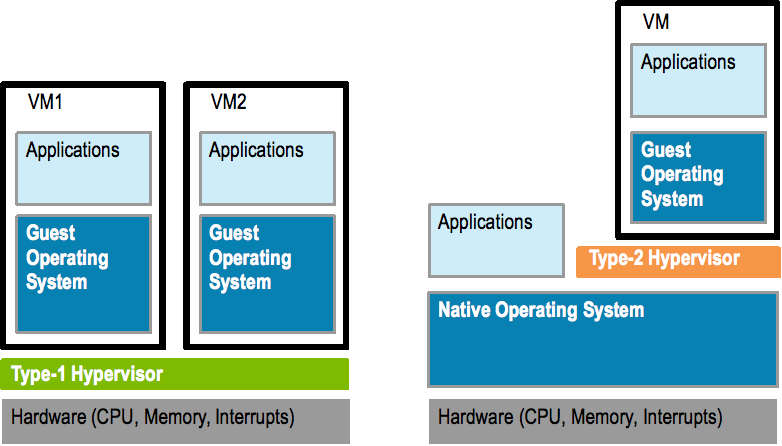
\includegraphics[width=0.8\maxwidth]{../figures/type1-vs-2.png}
    \caption{Hypervisor types\label{fig:hypervisors}}
   \end{center}
\end{figure}


\subsection{H μέθοδος Edge Orientation}

Full Virtualization is a hardware virtualization type on which the virtual
machine simulates almost completely the actual hardware to allow the guest
operating system software, mainly, to be run transparently and in isolation from
the rest system. That implies that every single feature of the physical hardware
can be reflected into a virtual machine, including interrupts, memory access,
and whatever other elements are used by the software that runs on the bare
machine.


\subsection{H μέθοδος Hausdorff Distance}

This technique does not simulates a hardware environment. However, the guest
applications are executed in their own isolated domains, as if they are running
on a separate system. With Paravirtualization the term of \emph{hypercall} is
introduced. The guest para-virtualized operating systems should make a system
call to the underlying hypervisor when it have to perform a privileged
operation. By allowing the guest OS to indicate its intents to the hypervisor,
improved performance and efficiency can be achieved, as each OS can cooperate to
obtain better performance when running in a virtual machine. As a result, the
guest OS have to be modified for the hypervisor, since the virtualization code
is integrated into the operating system itself. \emph{Xen} and \emph{User Mode
Linux} are examples of paravirtualization solutions.

\section{H μέθοδος Viola-Jones}\label{sec:violjon}

O αλγόριθμος των Viola-Jones~\cite{Viola01rapidobject} υπήρξε τομή στο πεδίο
της ανίχνευσης αντικειμένων σε εικόνες. Ουσιαστικά δημιούργησε την πρώτη
υποδομή ανίχνευσης αντικειμένων η οποία παρήγαγε ανταγωνιστικά αποτελέσμα σε
πραγματικό χρόνο. Παρόλο που σχεδιάστηκε ώστε να μπορεί να εκπαιδευτεί με σκοπό
να αναγνωρίζει οποιαδήποτε κλάση αντικειμένων, ουσιαστικά ο αρχικός σχεδιασμός
του αλγορίθμου έγινε με γνόμωνα την αναγνώρηση προσώπων σε εικόνες. Εν τέλει
εκεί εντοπίζεται και το μεγαλύτερο ποσοστό της χρήσης του.

Τα βασικά χαρακτηριστικά του ανωτέρο αλγορίθμου είναι:
\begin{description}
  \item[Αξιοπιστία] \hfill \\
      Ο αλγόριθμος έχει πάντα υψηλό ποσοστό σωστών ανιχνεύσεων (true-positives)
        και χαμηλό ποσοστό λάθος ανιχνεύσεων (false-ositives)
  \item[Ταχύτητα πραγματικού χρόνου] \hfill \\
      Σε εφαρμογές πραγματικού περιβάλλοντος επεξεργάζονται τουλάχιστον 2 εικόνες
        (frames) ανά δευτερόλεπτο
  \item[Αναγνώρηση προσώπων] \hfill \\
      Ο αλγόριθμος έχει στόχο να ανιχνέυει πρόσωπα από μη-πρόσωπα. Δεν έχει
        σκοπό να αναγνωρίζει τα πρόσωπα που ανιχνεύει
\end{description}

Για να το πετύχει αυτό ο αλγόριθμος χρησιμοποιεί κατά σειρά τα παρακάτω στάδια
τα οποία θα αναλύσουμε εκτενέστερα στη συνέχεια:
\begin{itemize}
 \item Επιλογή χαρακτηρισικών τύπου Haar (Haar features selection)
 \item Κατασκευή ολοκληρώματος εικόνας (Integral image creation)
 \item Εκπαίδευση του αλγορίθμου AdaBoost (AdaBoost training)
 \item Χρήση ενός διαδοχικά διασυνδεδεμένου ταξινομητή (Cascade classifier)
\end{itemize}

\subsection{Χαρακτηριστικά τύπου Haar}

Για να ανιχνεύσουμε αντικείμενα σε εικόνες απαιτείται κατάλληλη επεξεργασία και
αναπαράσταση του περιεχομένου τους. Για την αναπαράσταση του περιεχομένου της εικόνας στη
μέθοδο που εξετάζουμε, χρησιμοποιούμε τα χαρακτηριστικά τύπου Haar, τα οποία προκύπτουν
από την εφαρμογή του μετασχηματισμού κυματιδίων σε μια εικόνα με χρήση των συναρτήσεων
τύπου Haar~\cite{Viola01rapidobject}.

Η χρησιμοποίηση των συναρτήσεων Haar στο μετασχηματισμό κυματιδίων ξεκινά από την
παρατήρηση ότι η τιμή της φωτεινότητας κάθε εικονοστοιχείου επηρεάζεται έντονα από τις
        αλλαγές στο φωτισμό της σκηνής~\cite{OrePapSinOsu97}. Αυτή η αλλαγή όμως, επηρεάζει αρκετά ομοιόμορφα
όλα τα εικονοστοιχεία της εικόνας. Έτσι, η τιμή μιας συνάρτησης που εξετάζει τη μέση διαφορά
ανάμεσα σε δύο ή τρεις περιοχές της ίδιας εικόνας, θα παραμένει σε μεγάλο βαθμό ανεπηρέαστη.
Χρησιμοποιώντας, λοιπόν, τις συναρτήσεις Haar, η διαδικασία της ανίχνευσης αντικειμένων δε θα
επηρεάζεται από τις διαφορές στη φωτεινότητα από εικόνα σε εικόνα.

Οι συναρτήσεις Haar υπολογίζουν τη διαφορά ανάμεσα στους μέσους όρους των τιμών των
εικονοστοιχείων δύο (ή τριών) περιοχών. Ας θεωρήσουμε τη συνάρτηση Haar που παριστάνεται με
το ορθογώνιο i από το Σχήμα 2.1. Υπολογίζεται ο μέσος όρος των εικονοστοιχείων που
βρίσκονται μέσα στο άσπρο ορθογώνιο, καθώς και αυτών που βρίσκονται μέσα στο μαύρο
ορθογώνιο. Έπειτα, ο μέσος όρος του μαύρου ορθογωνίου αφαιρείται από τον μέσο όρο του
άσπρου. Η τιμή που προκύπτει αποτελεί την τιμή του Haar χαρακτηριστικού.

Εφαρμόζοντας τον μετασχηματισμό κυματιδίων με τη συναρτησιακή βάση Haar, προκύπτει
ένας περιορισμένος αριθμός χαρακτηριστικών~\cite{OrePapSinOsu97}. Στο μονοδιάστατο μετασχηματισμό, η
απόσταση ανάμεσα σε δύο γειτονικά κυματίδια, σε επίπεδο n , θα είναι 2 n . Η απόσταση αυτή είναι
πολύ μεγάλη, κι έτσι δεν λαμβάνουμε όσες πληροφορίες θέλουμε από μια εικόνα ώστε να την
- 21 -περιγράψουμε λεπτομερώς. Για να έχουμε, λοιπόν, μια πιο λεπτομερή, χωρικά, αναπαράσταση του
περιεχομένου της εικόνας χρειαζόμαστε ένα σύνολο από πλεονάζουσες συναρτήσεις βάσης. Για να
το πετύχουμε αυτό, εφαρμόζουμε τις συναρτήσεις Haar με μεταξύ τους απόσταση ένα
εικονοστοιχείο κάθε φορά. Έτσι, θα έχουμε μια πολύ πιο πυκνή αναπαράσταση. Επίσης, στο
μετασχηματισμό κυματιδίων, το μέγεθος των συναρτήσεων Haar, κανονικά διπλασιάζεται σε κάθε
επανάληψη. Για να αυξήσουμε ακόμα περισσότερο την λαμβανόμενη πληροφορία από την εικόνα,
ορίζουμε ότι το μέγεθος των συναρτήσεων Haar θα αυξάνει κάθε φορά κατά ένα μόνο
εικονοστοιχείο. Έτσι, το σύνολο των χαρακτηριστικών Haar σε μία εικόνα γίνεται
υπερπολλαπλάσιο του αρχικού. Αυξάνουμε, δηλαδή, την ποσότητα της πληροφορίας που αντλούμε
από μια εικόνα, αυξάνοντας τα χαρακτηριστικά τύπου Haar που θα υπολογιστούν σε αυτήν.

Τα κλασσικά Haar χαρακτηριστικά φαίνονται στο Σχήμα 2.1α ~\cite{OrePapSinOsu97}. Είναι σχετικά απλά
και μπορούν να εντοπίσουν ακμές οριζόντια και κατακόρυφα καθώς και διαγώνιες γραμμές. Για να
μπορέσουμε να αναπαραστήσουμε γραμμές, ράβδους και τετράγωνα καλύτερα, προσθέτουμε τα
χαρακτηριστικά που φαίνονται στο Σχήμα 2.1β (τα χαρακτηριστικά iv και v εμφανίζονται στο
~\cite{Viola01rapidobject}, ενώ τα υπόλοιπα στο ~\cite{Lienhart02anextended},
τα οποία υπολογίζονται χωρίς να αυξάνεται ιδιαίτερα η
πολυπλοκότητα, όπως θα δούμε στην ενότητα 2.2. Μια μεγάλη προσθήκη είναι τα χαρακτηριστικά
που είναι περιστραμμένα κατά 45 0 και φαίνονται στο Σχήμα 2.1γ ~\cite{Lienhart02anextended}. Με τη χρήση αυτών
βελτιώνεται σημαντικά η αναπαράσταση των διαγώνιων σχημάτων. Με την προσθήκη όλων αυτών
των χαρακτηριστικών, το σύνολο γίνεται υπερπλήρες και αναπαριστά πολύ καλύτερα την
πληροφορία που περιέχεται σε μία εικόνα.

Although the Cloud Computing became known to the public the last decade, that
does not constitutes a new invention or a revolution for the computer science.
It is more an evolution of already existing technologies rather than a new
computing paradigm. The following short historical review of the development of
computers and the Internet will show us that the idea of a centralized computer
utility was always existed and inevitably lead us to the beginning of Cloud
Computing~\cite{cloud_evolution}.


\begin{figure}[htbp]
  \begin{center}
    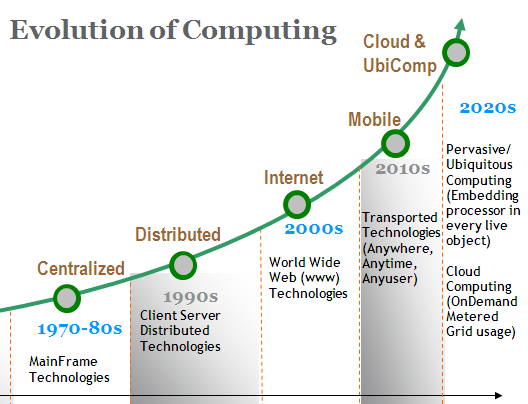
\includegraphics[width=0.75\maxwidth]{../figures/comp_evol.png}
    \caption{Computer history timeline\label{fig:comp_evol}}
   \end{center}
\end{figure}

Για τον υπολογισμό του πλήθους των Haar χαρακτηριστικών σε κάποιο παράθυρο εικόνας
πλάτους W και ύψους H, ακολουθούμε την παρακάτω διαδικασία [LiMa02]. Έστω ότι w και h
είναι το πλάτος και ύψος του ορθογωνίου της συνάρτησης Haar που εξετάζουμε. Το μέγεθος του
ορθογωνίου θα αυξάνεται κατά ένα σε κάθε βήμα. Άρα, οι μέγιστοι συντελεστές μεγέθυνσης των
 W 
 H 
ορθογωνίων σε πλάτος και ύψος θα είναι X =   και Y =   , αντίστοιχα. Το πλήθος των
 w 
 h 
χαρακτηριστικών που προκύπτουν από την εφαρμογή ενός κατακόρυφου Haar χαρακτηριστικού
στο παράθυρο εικόνας, είναι:


\begin{table}[htbp]
  \centering
  \begin{tabular}{ | l | l | }
    \hline
    Component & Description \\ \hline \hline
    CPU & 8 x QEMU Virtual CPU Version 1.7.0 \\
    \hline
    RAΜ & 8192 MB  \\
    \hline
    Disk & 80 GB \\
    \hline
  \end{tabular}
  \caption{Test-VM hardware specs}
  \label{tab:hw-specs}
\end{table}


\subsection{Ολοκλήρωμα εικόνας}

Cloud computing services can be classified along different layers, according to
the level of the capability they provide. There are three primary models, as
shown in Figure~\ref{fig:cloud_layers}, namely: Infrastructure as a Service
(\emph{IaaS}), Platform as a Service (\emph{PaaS}), and Software as a Service
(\emph{SaaS}). These abstraction levels can also be viewed as a layered
architecture where services of higher levels can be composed from the underlying
layers.

\begin{figure}[htbp]
  \begin{center}
    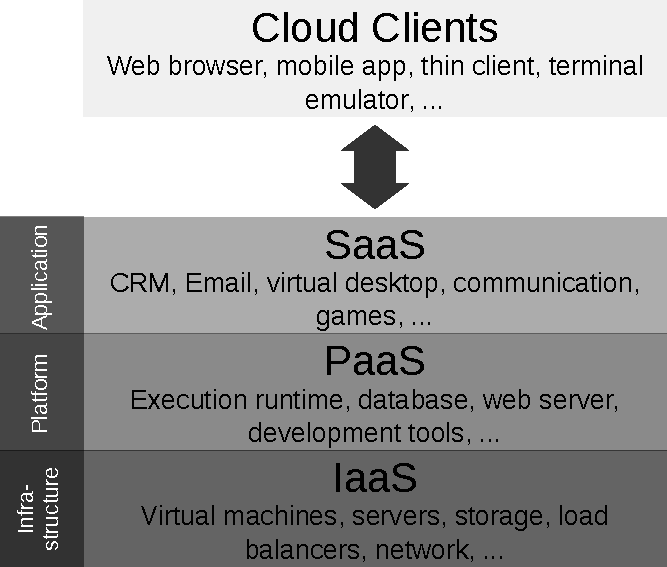
\includegraphics[width=1.0\maxwidth]{../figures/cloud_layers-black.pdf}
    \caption{The layers of Cloud Computing\label{fig:cloud_layers}}
   \end{center}
\end{figure}


\subsection{Ο αλγόριθμος AdaBoost}

Υπάρχουν πολλές μέθοδοι για την υλοποίηση ενός ταξινομητή, δεδομένου ενός συνόλου
χαρακτηριστικών και ενός συνόλου εκμάθησης θετικών και αρνητικών εικόνων. Έχουν
χρησιμοποιηθεί νευρωνικά δίκτυα, μηχανές διανυσμάτων υποστήριξης κ.α. Όπως είδαμε
προηγουμένως, τα χαρακτηριστικά που χρησιμοποιούμε μπορούν να υπολογιστούν πάρα πολύ
γρήγορα. Το σύνολο όμως των χαρακτηριστικών είναι πολύ μεγάλο (περίπου 120.000 για μια
εικόνα 20x20). Έτσι, ο υπολογισμός του πλήρους συνόλου των χαρακτηριστικών για την ανίχνευση
σε κάθε υποπαράθυρο της εικόνας, θα ήταν και πάλι πολύ χρονοβόρος [ViJo01]. Θα πρέπει,
λοιπόν, να επιλέξουμε ένα μικρό αριθμό χαρακτηριστικών από το διαθέσιμο σύνολο, και να
- 27 -κατασκευάσουμε από αυτά τον ταξινομητή μας. Η επιλογή αυτών των χαρακτηριστικών είναι
αρκετά δύσκολη.

Στην μέθοδο ανίχνευσης που εξετάζουμε, χρησιμοποιήθηκε ο αλγόριθμος AdaBoost τόσο για
την επιλογή των χαρακτηριστικών που θα χρησιμοποιηθούν, όσο και για την εκπαίδευση του
ταξινομητή [FrSc95]. Ο αλγόριθμος εκμάθησης AdaBoost ανήκει στην κατηγορία των
αλγορίθμων ενδυνάμωσης (boosting) και χρησιμοποιείται για να αυξήσει την απόδοση ενός
οποιουδήποτε απλού αλγορίθμου ταξινόμησης. Ο απλός αλγόριθμος ταξινόμησης λέγεται και
ασθενής αλγόριθμος ταξινόμησης, καθώς ακόμα και η καλύτερη συνάρτηση ταξινόμησης που
μπορεί να προκύψει από αυτόν, δεν αναμένεται να ταξινομεί καλά τα δεδομένα. Συγκεκριμένα,
αρκεί η συνάρτηση ταξινόμησης να έχει απόδοση ελαφρά καλύτερη από την τυχαία ταξινόμηση
(50%). Για να αυξήσει, λοιπόν, την απόδοση ενός ασθενούς αλγορίθμου ταξινόμησης, ο AdaBoost
συνδυάζει μια συλλογή ασθενών συναρτήσεων ταξινόμησης χρησιμοποιώντας άπληστο αλγόριθμο,
ώστε να σχηματίσει από αυτούς έναν ισχυρότερο ταξινομητή.

Η βελτίωση του ασθενούς αλγορίθμου ταξινόμησης πραγματοποιείται, καλώντας τον
αλγόριθμο να επιλύσει μια αλληλουχία προβλημάτων ταξινόμησης. Αρχικά, όλα τα παραδείγματα
(θετικά και αρνητικά) παίρνουν μια τιμή βάρους, η οποία είναι ίδια για όλα. ∆ίνονται στον
αλγόριθμο τα παραδείγματα και πραγματοποιείται ο πρώτος κύκλος εκμάθησης, όπου ο
αλγόριθμος ταξινομεί όλα τα παραδείγματα με κάθε διαθέσιμη συνάρτηση ταξινόμησης. Έπειτα,
οι συναρτήσεις ταξινόμησης διατάσσονται σύμφωνα με τα αποτελέσματά τους, λαμβάνοντας υπόψη
το βάρος κάθε παραδείγματος. Επιλέγεται ένας μικρός αριθμός συναρτήσεων ταξινόμησης, από
αυτές με τα καλύτερα αποτελέσματα, που αποτελούν τον πρώτο ασθενή ταξινομητή. Ο πρώτος
κύκλος εκμάθησης ολοκληρώνεται και τα βάρη των παραδειγμάτων ισοσταθμίζονται, δίνοντας
μεγαλύτερο βάρος στα παραδείγματα που ταξινομήθηκαν λανθασμένα από τον πρώτο ασθενή
ταξινομητή. Έτσι, στον δεύτερο κύκλο εκμάθησης ο αλγόριθμος ταξινόμησης θα θεωρήσει πιο
σημαντικά τα παραδείγματα που ταξινομήθηκαν λανθασμένα από τον προηγούμενο ταξινομητή.
Τα βήματα επαναλαμβάνονται διαδοχικά, μέχρι να φτάσουμε στο επίπεδο του συνολικού λόγου
λανθασμένης ταξινόμησης που επιθυμούμε. Τελικά, ο ισχυρός ταξινομητής προκύπτει από τον
συνδυασμό των ασθενών ταξινομητών που επιλέχθηκαν και ένα κατώφλι. Κατά την διαδικασία της
ταξινόμησης ενός υποπαραθύρου εικόνας από τον ισχυρό ταξινομητή, εφαρμόζονται στο
υποπαράθυρο όλοι οι ασθενείς ταξινομητές. Τα αποτελέσματα των ασθενών ταξινομητών
αθροίζονται, και αν το άθροισμα ξεπερνά το κατώφλι του ταξινομητή, το υπό εξέταση αντικείμενο
ταξινομείται ως θετικό, αλλιώς ως αρνητικό.

Υπάρχουν τέσσερις εκδοχές του αλγόριθμου AdaBoost [FrHT00]. Η αρχική εκδοχή
ονομάζεται ∆ιακριτός AdaBoost (Discrete AdaBoost – DAB) καθώς η συνάρτηση ταξινόμησης
κάθε ασθενή ταξινομητή παίρνει μόνο δύο διακριτές τιμές, τις { − 1,1  } ανάλογα με το αν ένα
δείγμα ταξινομείται ως θετικό ή αρνητικό. Η δεύτερη εκδοχή ονομάζεται Πραγματικός AdaBoost
(Real AdaBoost – RAB), καθώς η συνάρτηση ταξινόμησης κάθε ασθενή ταξινομητή παίρνει όλες
τις πραγματικές τιμές στο διάστημα [ 0,1  ] . Με τη χρήση του RAB, μπορούμε να έχουμε μια
ένδειξη εμπιστοσύνης για τα αποτελέσματα της ταξινόμησης, χρησιμοποιώντας τις τιμές που
επιστρέφονται από τον αλγόριθμο και όχι μόνο το αποτέλεσμα της θετικής ή αρνητικής
ταξινόμησης. Άλλη εκδοχή είναι ο Ήπιος AdaBoost (Gentle AdaBoost – GAB), ο οποίος
βασίζεται στον Πραγματικό AdaBoost αλλά χρησιμοποιεί βήματα της μεθόδου Newton αντί για
ακριβή υπολογισμό. Τέλος, υπάρχει και ο LogitBoost, ο οποίος έχει δύο παραλλαγές, αυτή που
χρησιμοποιεί δύο κλάσεις και αυτή που χρησιμοποιεί J κλάσεις. Ο αριθμός των κλάσεων επηρεάζει
- 28 -την τιμή της εκτίμησης πιθανότητας κάθε δείγματος x i , η οποία ισούται με p ( x i  ) =
1
στη μία
2
1
στην άλλη.
J

Στη μέθοδο ανίχνευσης αντικειμένων που χρησιμοποιούμε, κάθε ασθενής αλγόριθμος
εκμάθησης περιορίζεται στο σύνολο των συναρτήσεων ταξινόμησης που αποτελούνται από ένα
μόνο χαρακτηριστικό τύπου Haar. Προφανώς, από ένα μόνο χαρακτηριστικό δε μπορούμε να
περιμένουμε ιδιαίτερα χαμηλό λόγο σφάλματος. Σε κάθε στάδιο του αλγορίθμου AdaBoost
επιλέγεται το χαρακτηριστικό που διαχωρίζει καλύτερα τα θετικά από τα αρνητικά δείγματα. Για
κάθε χαρακτηριστικό, ο ασθενής αλγόριθμος εκμάθησης προσδιορίζει ένα κατώφλι της τιμής του
χαρακτηριστικού, που ελέγχοντάς το περιορίζονται οι λανθασμένες ταξινομήσεις από το
συγκεκριμένο χαρακτηριστικό στις ελάχιστες δυνατές. Έπειτα, επιλέγεται ως ασθενής ταξινομητής
το χαρακτηριστικό τύπου Haar, που, για το δεδομένο κατώφλι του, κάνει τη συνολικά καλύτερη
ταξινόμηση. Ο AdaBoost συνεχίζει εκπαιδεύοντας όλους τους ασθενείς ταξινομητές, μέχρι το
σημείο που ο ισχυρός συνολικός ταξινομητής επιτυγχάνει το επίπεδο ταξινόμησης που ζητάμε.
Ο αλγόριθμος AdaBoost παρέχει αρκετά ισχυρές εγγυήσεις για την ορθότητά του. Έχει
αποδειχθεί, ότι το σφάλμα ταξινόμησης του ισχυρού ταξινομητή που προκύπτει από την εφαρμογή
του αλγορίθμου, τείνει προς το μηδέν εκθετικά ως προς τον αριθμό των κύκλων εκπαίδευσης
[SFBL98]. Επίσης, η όλη διαδικασία της εκμάθησης πραγματοποιείται με μεγάλη ταχύτητα. Ας
θεωρήσουμε ότι έχουμε στη διάθεσή μας K χαρακτηριστικά τύπου Haar και
εικόνες-
παραδείγματα. Για να κατασκευαστεί ένας ισχυρός ταξινομητής από τον αλγόριθμο AdaBoost,
περίπτωση και p ( x i  ) =
που αποτελείται από M ασθενείς ταξινομητές, χρειάζονται O ( M K  ) βήματα, σε αντίθεση με
άλλους αλγορίθμους που χρειάζονται O ( M K
)
βήματα.

\subsection{Χρήση ενός Cascade Classifier}

Σε αυτή την ενότητα παρουσιάζεται η μέθοδος ταξινόμησης με χρήση ενός ∆ιαδοχικά
Συνδεδεμένου Ταξινομητή (∆ΣΤ) [ViJo01]. Η μέθοδος αυτή βοηθά στη επίτευξη υψηλού λόγου
ανίχνευσης, μειώνοντας σημαντικά τον απαιτούμενο χρόνο. Η ιδέα στηρίζεται στο γεγονός ότι
μπορούμε να κατασκευάσουμε πολλούς μικρούς σε μέγεθος ταξινομητές, τους οποίους θα
συνδέσουμε διαδοχικά. Μπορούμε, λοιπόν, να χρησιμοποιήσουμε απλούστερους και πολύ
γρήγορους ταξινομητές αρχικά, οι οποίοι θα απορρίπτουν γρήγορα την πλειονότητα των
αρνητικών υποπαραθύρων, και πιο σύνθετους και χρονοβόρους αργότερα, ώστε να μειώσουμε το
λόγο λανθασμένων ανιχνεύσεων.

Η διάταξη του ∆ΣΤ θυμίζει τη μορφή ενός εκφυλισμένου δέντρου απόφασης. Κάθε
υποπαράθυρο της εικόνας εισέρχεται στον πρώτο ταξινομητή. Αν ο ταξινομητής το κατατάξει ως
θετικό, αυτό περνά ως είσοδος στον δεύτερο ταξινομητή. Αν και αυτός το κατατάξει ως θετικό,
τότε περνά στον τρίτο κ.ο.κ. Αν σε αυτή τη διαδοχή κάποιος ταξινομητής κατατάξει το
υποπαράθυρο ως αρνητικό, τότε αυτό απορρίπτεται και δεν εξετάζεται από κανένα άλλο
ταξινομητή (βλέπε Σχήμα 2.4). Θα μπορούσαμε να παρομοιάσουμε τον ∆ΣΤ με έναν μεγάλο
ταξινομητή που αποτελείται από το σύνολο των χαρακτηριστικών του ∆ΣΤ, όπου όμως δεν
περιμένουμε να υπολογιστεί όλο το πλήθος των χαρακτηριστικών. Αντίθετα, ελέγχουμε ανά μερικά
- 29 -χαρακτηριστικά το άθροισμα των τιμών των χαρακτηριστικών για να αποφασίσουμε αν το υπό
εξέταση υποπαράθυρο απορρίπτεται ή όχι.

\begin{figure}[htbp]
  \begin{center}
    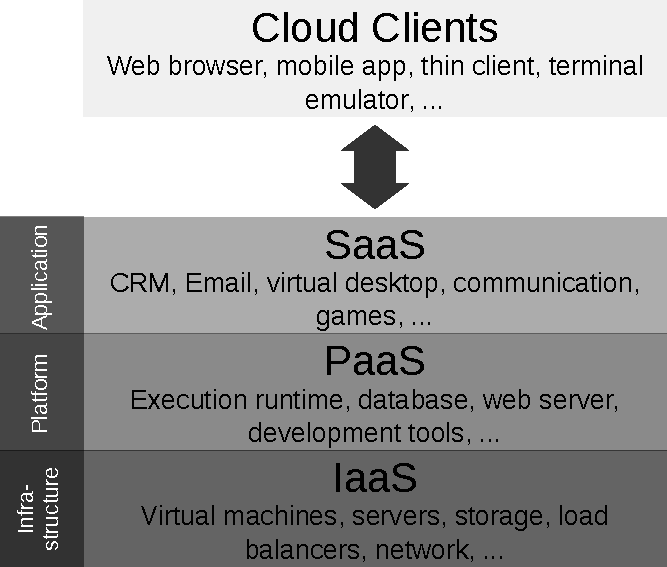
\includegraphics[width=1.0\maxwidth]{../figures/cloud_layers-black.pdf}
    \caption{The layers of Cloud Computing\label{fig:cloud_layers}}
   \end{center}
\end{figure}
\section{Άλλες μέθοδοι που έχουν χρησιμοποιηθεί}\label{sec:othermethods}

Κάθε ταξινομητής του ∆ΣΤ εκπαιδεύεται χρησιμοποιώντας ένα σύνολο θετικών και ένα
σύνολο αρνητικών παραδειγμάτων, όπως είδαμε στην ενότητα 2.3. Το σύνολο των θετικών
παραδειγμάτων είναι το ίδιο κατά την εκπαίδευση κάθε ταξινομητή. Το σύνολο των αρνητικών
παραδειγμάτων όμως, μεταβάλλεται. Συγκεκριμένα, κάθε ταξινομητής εκπαιδεύεται
χρησιμοποιώντας ως αρνητικά παραδείγματα, τα παραδείγματα που ταξινομούνται από τους
προηγούμενους ταξινομητές του ∆ΣΤ ως θετικά [ViJo01]. Αυτό αυξάνει σε πολύ μεγάλο βαθμό τα
αρνητικά παραδείγματα τα οποία θα εξεταστούν συνολικά. Για να φτάσει ένας συγκεκριμένος
αριθμός αρνητικών παραδειγμάτων στον τρέχοντα ταξινομητή, θα πρέπει τα παραδείγματα αυτά
να ταξινομηθούν από όλους τους προηγούμενους ταξινομητές του ∆ΣΤ (λανθασμένα) ως θετικά.
Ας θεωρήσουμε ότι σε κάθε στάδιο ενός ∆ΣΤ θέλουμε να εξετάζονται 1.000 αρνητικά
παραδείγματα και κάθε στάδιο έχει λόγο λανθασμένης θετικής ανίχνευσης 0,5. Τότε, για να
περάσουν στο δέκατο στάδιο 1.000 αρνητικά παραδείγματα, αυτά θα χρειαστεί να έχουν
ταξινομηθεί από τα προηγούμενα εννιά στάδια ως θετικά. Έτσι, συνολικά θα πρέπει να εξεταστούν
περίπου 512.000 αρνητικά παραδείγματα.

Η εξέταση πολύ μεγαλύτερου αριθμού αρνητικών παραδειγμάτων αυξάνει την τελική απόδοση
του ∆ΣΤ. Αντίθετα, κάθε ταξινομητής καλείται να πραγματοποιήσει μια πιο δύσκολη ταξινόμηση
από αυτές των προηγούμενων ταξινομητών. Τα αρνητικά παραδείγματα που θα έχει στη διάθεσή
του θα είναι πιο δύσκολα στην ταξινόμηση από τα παραδείγματα που είχαν τα προηγούμενα από
αυτό στάδια. Έχοντας, λοιπόν, πιο δύσκολο σύνολο εκπαίδευσης ένας ταξινομητής που βρίσκεται
σε προχωρημένο στάδιο, θα παρουσιάσει αυξημένες λανθασμένες ταξινομήσεις, θετικές και
αρνητικές.

Οι απλοί ταξινομητές ενός ∆ΣΤ, θα πρέπει να έχουν πολύ χαμηλό λόγο λανθασμένων
αρνητικών ταξινομήσεων, ώστε να μην χάνονται τα πραγματικά αντικείμενα στη συνολική
ταξινόμηση. Για να διασφαλίσουμε τη σωστή λειτουργία του ∆ΣΤ, θα πρέπει να αυξήσουμε
περαιτέρω τις θετικές ταξινομήσεις (είτε αφορούν πραγματικά αντικείμενα είτε όχι) [ViJo01]. Μια
τεχνική για να πετύχουμε αυτό το αποτέλεσμα είναι να επέμβουμε στις τιμές των κατωφλίων των
ταξινομητών που προσδιόρισε ο αλγόριθμος AdaBoost κατά την εκπαίδευση. Το κατώφλι ενός
ταξινομητή ορίζει την ελάχιστη τιμή του σταθμισμένου με βάρη αθροίσματος των τιμών των
χαρακτηριστικών που θα πρέπει να έχει ένα υποπαράθυρο για να ταξινομηθεί ως θετικό. Ένα
υποπαράθυρο ταξινομείται, δηλαδή, ως θετικό, όταν το (σταθμισμένο) άθροισμα των τιμών των
- 30 -χαρακτηριστικών που υπολογίστηκε για αυτό ξεπερνά το κατώφλι του ταξινομητή. Έτσι,
μειώνοντας τις τιμές των κατωφλίων θα αυξηθεί ο αριθμός των παραθύρων που ταξινομούνται ως
θετικά, άρα και ο λόγος θετικών ταξινομήσεων

\subsection{NoSQl compromises}

Companies want solutions that would scale, be fast, and operationally efficient.
They also ideally expect operations to speed up by simply adding new commodity
hardware, at almost a linear rate. One major bottleneck to accomplish that goal
are the database systems. So, in order to achieve the desired behavior, some
compromises should be made, and a bunch of tradeoffs should be taking into
account~\cite{burd}.

\begin{description}\label{item:cap}
  \item[The CAP Theorem] \hfill \\
    In \emph{2000}, Berkeley's CA researcher Eric Brewer published the CAP
    Theorem~\flink{http://en.wikipedia.org/wiki/CAP\_theorem}, also known as
    Brewer's Theorem. What Brewer claimed is that it is impossible for a
    distributed system to continually maintain perfect \emph{C}onsistency,
    \emph{A}vailability, and \emph{P}artition tolerance.

    \begin{itemize}
      \item \emph{Consistency}: All node see the same data at the same time.
      \item \emph{Availability}: A guarantee that every request receives a
            response about whether it was successful or failed.
      \item \emph{Partition tolerance}: The system will continue to operate
            despite arbitrary message losses.
    \end{itemize}

    The theorem states that when designing a database distributed system you
    must make tradeoffs among the above features because you cannot
    simultaneously maintain all three of them. Peter Mell, a senior computer
    scientist for the National Institute of Standards and Technology (NIST),
    said that:

    \begin{flushright}
      \emph{In the database world, they can give you perfect consistency, but
            that limits your availability or scalability. It’s interesting, you
            are actually allowed to relax the consistency just a little bit, not
            a lot, to achieve greater scalability.}

      \emph{Well, the big data vendors took this to a whole new extreme. They
            said that we are going to offer amazing availability or scalability,
            knowing that the data is going to be consistent eventually, usually.
            That was great for many things.}~\cite{peter_mell}
    \end{flushright}

    What Mell actually said is that maybe we need a balance. So systems should
    be developed with CAP tradeoffs, relative to operations that the product
    provides, rather than relative to the product as a whole. This is what a
    NoSQL solution actually does. It employs less constrained consistency models
    than traditional relational databases, but with higher availability and
    partition-tolerance.

  \item[ACID vs BASE] \hfill \\
    In distributed systems where there is a great deal of communication involving
    locks, scalability can not be easily achieved. One solution is to relax the
    consistency property and pass from \emph{``strong"} consistency to something
    called \emph{``eventual"} consistency. This actually means that updates made
    by a part of a
    system should become known to the rest parts of the system within a short
    period of time and not directly after the transaction is completed. For many
    applications the acknowledgment that the information will eventually arrive
    to all nodes satisfy the requirements. One other approach is using a concurrency
    control method called \emph{Multi Version Concurrency Control (MVCC)}
    \flink{http://en.wikipedia.org/wiki/Multiversion\_concurrency\_control}.
    Both of those techniques add an extra overhead to the programmer of
    the application who is responsible of dealing with the coming information
    appropriately. An another property is durability. Many NoSQL solutions
    choose not to save data to disk at once, because writing to disk slows down
    the whole system, but keeping them in memory instead. A balance should be
    found between durability and speed of performing read/write operations.
    Eventually, that approach keeps a small window open where seemingly committed
    transactions can be lost. Many other approaches designed, but as with any
    other databases, when evaluating a NoSQL solution, you should choose depending
    on your application requirements~\cite{burd}.


    Figure~\ref{fig:cap}, sums up everything discussed in the current subsection
    in a single image.

    \begin{figure}[htbp]
      \begin{center}
        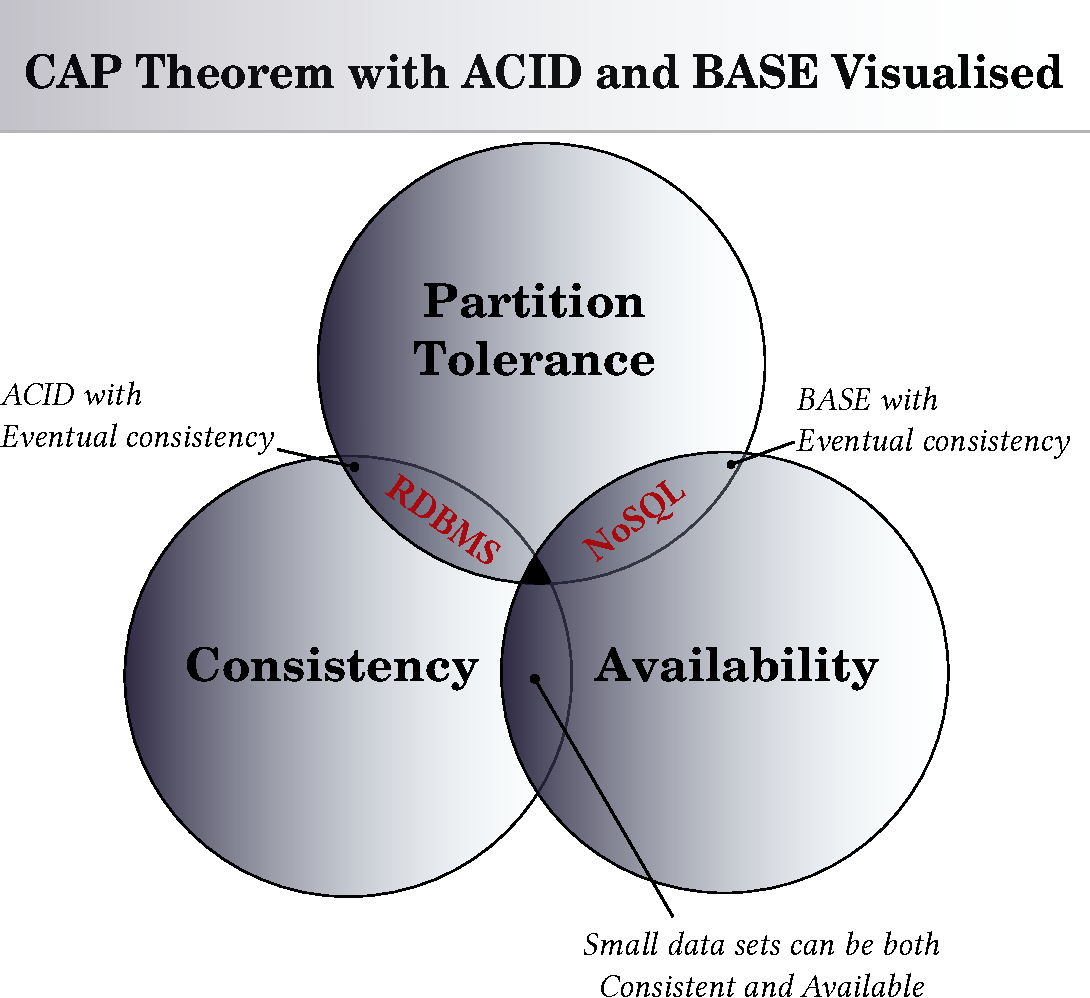
\includegraphics[width=0.8\maxwidth]{../figures/cap-nist.pdf}
        \caption{CAP theorem with ACID and BASE visualized\label{fig:cap}}
       \end{center}
    \end{figure}
\end{description}

\subsection{NoSQL Models}


\chapter{Ganeti backend}\label{ch:ganeti}

This chapter concentrates on Ganeti. We will discuss the architecture of Ganeti,
and we will analyze in details its most basic parts and how they interact with
each other. We will try to provide small documentation to familiarize the reader
with this tool, avoiding presenting superfluous information. Summing up, the
objective for the reader is at the end of this chapter to have a comprehensive
view of Ganeti and its basic structure.

\section{Overview}

Ganeti is a software tool to manage computer clusters, and also assumes the
management task of the virtual instances of the cluster. Is is being
developed by Google and is an Open Source Project since 2007. It is build on top
of existing virtualization technologies, such as XEN or KVM hypervisors, and
other open source software. It also uses LVM for disk management, optionally
DRBD for disk replication across physical hosts, and other disk templates such
as RBD, external shared storage providers and more.

Ganeti uses a daemon-based model. Each daemon deals with specific tasks that the
cluster has to face, and communicates with other daemons using various
protocols, mainly HTTP based, and custom ones like LUXI. Many of those daemons
are written in Haskell, but most of the project's code is in Python. Ganeti is
actually a wrapper around hypervisors. Once installed, the tool will take over
the management part of virtual instances. It also makes it convenient for system
administrators to setup and handle clusters of physical nodes.

Some of the main features that Ganeti provides, and controls are the following:

\begin{itemize}
  \item Cluster management of physical nodes.
  \item Support for XEN virtualization.
  \item Support for KVM virtualization.
  \item Support for virtual console to control instances ,e.g, VNC.
  \item Support for live instance migration.
  \item Support for virtio or emulated devices.
  \item Disk management: plain LVM volumes, files, Across-the-network RAID1
        (using DRBD) for quick recovery in case of physical system failure.
  \item Export/import mechanisms for backup purposes or migration between
        cluster.
  \item Fast and simple recovery after physical failures using commodity
        hardware.
\end{itemize}

\section{Terminology}

In this section, we provide a small introduction of the most basic Ganeti terms,
in order to facilitate the reader in the rest of the document. In
Figure~\ref{fig:gnt_abst}, we present an abstract Ganeti architecture, which will
help us to briefly explain those terms.

\begin{figure}[htbp]
  \begin{center}
    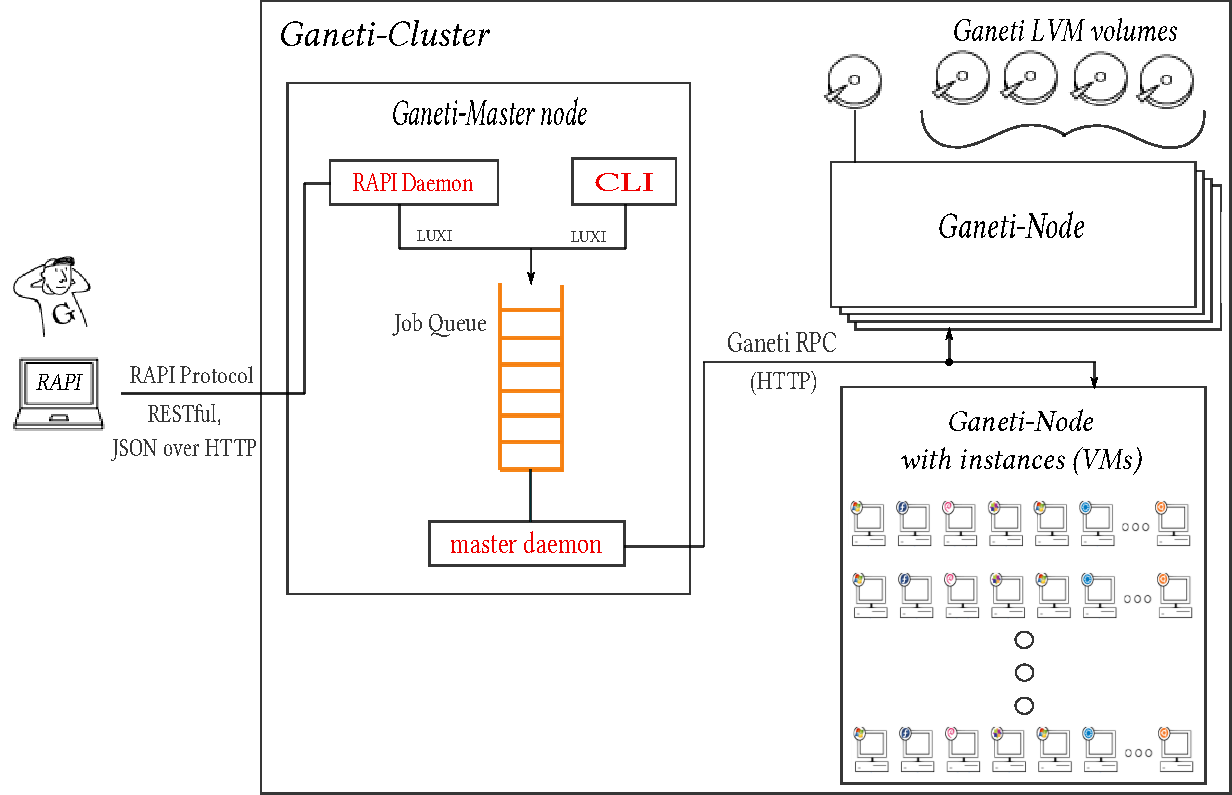
\includegraphics[width=1.0\maxwidth]{../figures/ganeti_abst_arch.pdf}
    \caption{Ganeti base components, version 2.7.2\label{fig:gnt_abst}}
   \end{center}
\end{figure}

\begin{description}
  \item[Cluster] \hfill \\
    A set of computers (nodes) working together to provide a coherent, reliable,
    scalable, highly-available virtualization service under a single domain.
  \item[Node] \hfill \\
    A physical machine which corresponds to the basic cluster infrastructure. If
    they host no instances, nodes can be added and removed at will from the
    cluster. They do not have to be fault-tolerant in order to achieve
    high availability for the instances they host. The loss of a single node,
    in a HA cluster, will not cause disk data loss for any of the instances it
    hosts.

    A node belonging to a cluster can serve different roles; VM-hosting and/or
    Administrative roles, which will be explained later in this document.
    Independently of its role, nodes can be in different statuses like online,
    drained or offline. Depending on the role they serve, each node will run a
    set of daemons:

    \begin{itemize}
      \item ganeti-masterd
      \item ganeti-noded
      \item ganeti-rapid
      \item ganeti-confd
    \end{itemize}
  \item[Instance] \hfill \\
    A virtual machine that runs on a cluster. Instances in Ganeti are
    highly-available entities, that can also become fault-tolerant depending on
    the disk template they use, e.g., DRBD. An instance has various parameters
    which can be modified either at instance level or at cluster level via
    cluster default parameters. Those parameters can be classified in three
    main categories: hypervisor related parameters, called \texttt{hvparams},
    general parameters, called \texttt{beparams}, and network interface
    parameters, called \texttt{nics}.
  \item[Disk Template] \hfill \\
    The layout disk type for the instance. Instances in Ganeti see the same
    virtual drive in all cases, but the node-level configuration varies between
    them. The available storage templates are the following:
    \begin{description}
      \item[diskless] \hfill \\
        This creates an instance with no disks. Useful for testing purposes, or
        other special cases.
      \item[file] \hfill \\
        Disk devices will be regular plain files. No redundancy is provided.
      \item[sharedfile] \hfill \\
        Disk devices will be regular plain files under a shared directory. This
        option allows live migration and failover of instances.
      \item[plain] \hfill \\
        Disk devices will be LVM volumes.
      \item[drbd] \hfill \\
        Disk devices will be drbd on top of LVM volumes, compatible with DRBD
        versions 8.x.
      \item[rbd] \hfill \\
        Disk devices will be rbd volumes, short for RADOS block device, residing
        inside a RADOS cluster.
      \item[blockdev] \hfill \\
        Pre-existent block devices will be used as backend for its disks.
      \item[ext] \hfill \\
        The instance will use an external storage provider as disk backend,
        through the ExtStorage Interface, using ExtStorage providers.
    \end{description}
  \item[\emph{Primary} and \emph{Secondary} concepts] \hfill \\
    An instance has a primary node, and depending on the disk configuration
    chosen might also have a secondary one. Every DRBD instance runs in its
    primary node and uses the secondary for disk replication and
    fault-tolerance. When those terms used in node level, they refer to the
    instances having the given node as primary and secondary, respectively.
  \item[IAllocator] \hfill \\
    A framework for using external user-provided scripts to automatically
    compute the placement of new instances on the cluster nodes. This
    eliminates the need to manually specify the exact locations of an instance
    addition/move, and make the node evacuate operations an easy, and common
    cluster operation.

    In order for Ganeti to be able to use those scripts, we should place them
    under the \texttt{\$libdir/ganeti/iallocators} folder path.
  \item[Jobs and OpCodes] \hfill \\
    A \emph{Job} in Ganeti is the basic operation to modify the cluster's state.
    A job consists of multiple \emph{OpCodes} internally, short for ``Operation
    Code". This is the basic element of operation in Ganeti. Most of the
    commands in Ganeti are equivalent to one opcode, or in some cases a sequence
    of opcodes, all of the same type ,e.g., shutting down all instances in a
    cluster. The opcodes of a single job are processed serially, but different
    jobs can be executed in parallel, in different order than they have been
    submitted, depending on hardware resource availability, locks, or priority
    given by user.
\end{description}

\section{Architecture}\label{sec:architecture}

As we mentioned earlier in this section, Ganeti has a daemon-based architecture.
Every Ganeti-related command, (\texttt{gnt-*} commands), is an individual client
which ``talk" to the master daemon who executes every cluster operation.

In Figure~\ref{fig:gnt_arch}, we present the architecture of a Ganeti cluster in
a more detailed form than in Figure~\ref{fig:gnt_abst}, and we show how the most
basic daemons and elements interact with each other.

\begin{figure}[htbp]
  \begin{center}
    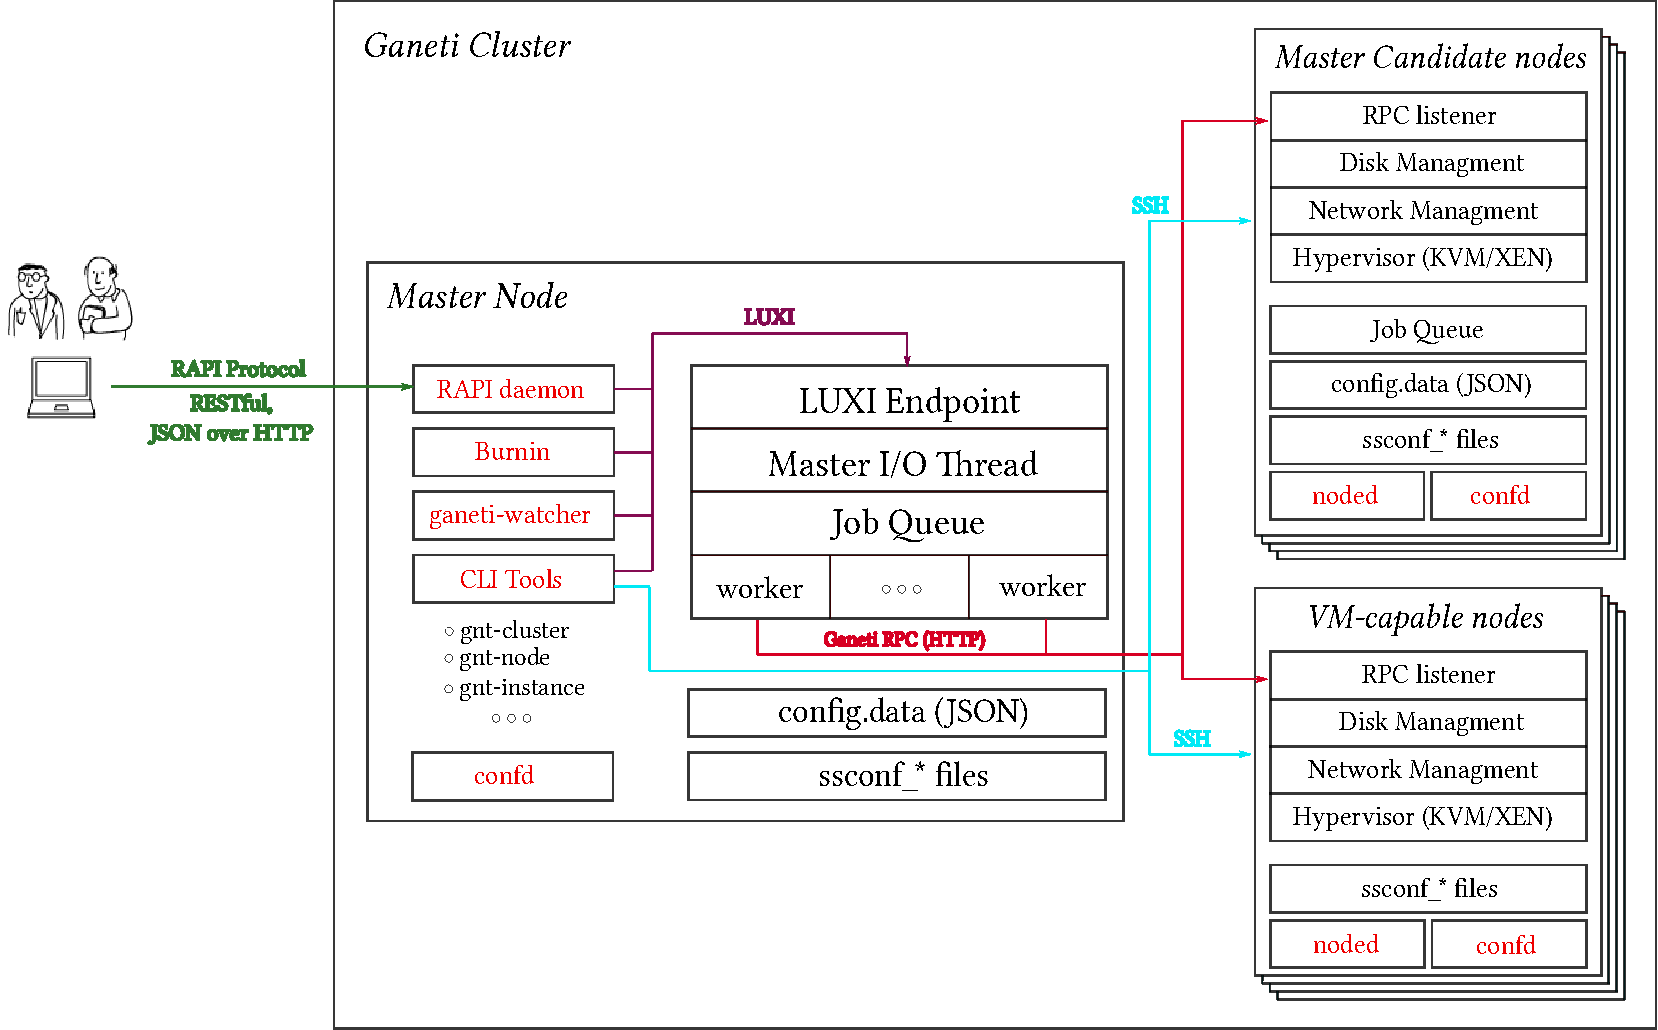
\includegraphics[width=1.0\maxwidth]{../figures/ganeti_arch_horizonal.pdf}
    \caption{Ganeti architecture, version 2.7.2\label{fig:gnt_arch}}
   \end{center}
\end{figure}

\emph{Nodes} are the basic cluster infrastructure in Ganeti. They serve
different roles and they can, and usually do, serve more than one. We could
group node roles into two major categories; The \emph{Administrative}
and the \emph{VM-capable} nodes. Nodes belonging in the first category, can
modify the cluster state, or take part in cluster related decisions like the
master node voting procedure. Nodes in second category can simply hosts
instances (VMs).

In more details, a node can belong in one, or more of the following roles:

\begin{description}
  \item[Master] \hfill \\
    It is the cluster coordinator node and it holds the authoritative copy of
    the cluster configuration. Every decision that could affect the cluster
    state managed by this node, because it is the only node which can execute
    commands. Only one master should exist every time in a Ganeti cluster.
  \item[Master Candidate] \hfill \\
    Nodes in this category have the full copy of the live cluster configuration
    and jobs. Only nodes belonging in this role can become master. This set of
    nodes called \emph{candidate pool}, and there is also a parameter called
    \texttt{candidate\_pool\_size}, which represents the number of candidates
    the cluster tries to maintain, automatically. Because the
    \texttt{candidate\_pool\_size} can have a huge impact in Ganeti performance,
    for reasons which we 'll explain later, it can be configured during
    initialization or modified via cluster related commands (\texttt{gnt-cluster
    *}).
  \item[Master Capable] \hfill \\
    Nodes in this category are not master candidates, but can become and
    promoted to master node, in cases when nodes in the candidate pool
    are less than the desired size. In such case, a randomly selected master
    capable node is promoted to master candidate. We could disable this flag
    and exclude some nodes from being master candidates in case when they have
    a less reliable hardware and we do not want to store sensitive information
    to them.
  \item[VM Capable] \hfill \\
    This is the default node state and means that the node can host instances.
    More specifically, the node will participate in instance allocation
    operations, capacity calculations, cluster checks, and other operations.
  \item[Offline] \hfill \\
    Nodes having this flag set have some special characteristics. They are still
    recorded in the Ganeti configuration, and can only take part in the
    master voting procedure, to ensure consistency. They are not allowed to
    become master. Enabling this flag to a master candidate node will demote
    it from candidate possibly, causing another node which is master capable to
    be promoted. Additionally, these nodes are not allowed to host primary
    instances. The main reason this role was added to Ganeti was to allow
    broken machines that are being repaired to remain in the cluster without
    introducing further problems.\\
  \item[Drained] \hfill \\
    Nodes in this state, will not participate in instance allocation operations,
    but all other operations as queries, or starting and stopping instances, are
    working without any restrictions. The actual intention is that nodes in this
    role have some issue and they are being evacuated for hardware repairs.
\end{description}

Previously, we made some references to Ganeti \emph{Cluster Configuration} and
\emph{Jobs} which are stored in the system as files. These files are stored
under the \texttt{/var/lib/ganeti} directory, and actually form a database for
the cluster. Every single piece of information that the cluster needs to operate
normally is stored in those files.

\subsection{Cluster Configuration}\label{subsec:config}

The cluster configuration is a set of files which are present in all, or a
subset of nodes depending on their usage. We could group them into three main
categories, namely:

\begin{description}
  \item[config.data] \hfill \\
  The cluster configuration database is a single JSON config file called
  \texttt{config.data}. The master node keeps a valid version of this file and
  it also replicates it to the master candidate nodes, for reliability
  reasons. Ganeti has a special way to handle \texttt{config.data} updates; It
  holds the \texttt{config.data} both in master memory and disk. The canonical
  version of the config exists at every moment in the master node memory, and
  the disk version will be updated from there. Every operation that updates a
  single object in the memory version of the \texttt{config.data}
  automatically causes a flush of the whole file to disk. If the config
  does not flushed successfully to disk, the operation will fail. The
  \texttt{config.data} file contains information about all the major Ganeti
  objects such as cluster, nodes, instances, networks, and their attributes.
  We will extensively talk about the \texttt{config.data} structure in the
  next chapters.

  \item[ssconf\_*] \hfill \\
  Besides the objects contained in the \texttt{config.data}, which change
  quite often, Ganeti also holds a set of configuration files which contain
  information that does not change frequently and needs to be present to all
  Ganeti nodes. These files are stored in the same directory as the
  \texttt{config.data} file and start with a \texttt{ssconf\_} prefix. For
  example, the ssconf file which contains the master IP value is called
  \texttt{ssconf\_master\_ip}, and so on. The main reason for the existence of
  the ssconf files is that the most frequent Ganeti operations should not need
  to contact the master node and overload him. In addition, we want some
  information to be accessible at every moment, even if the master node is
  down, so that we can use it from services external to the cluster, and
  avoiding the single point of failure that a master hard shutdown could
  introduce.

  \item[SSL certificates] \hfill \\
  Ganeti uses OpenSSL for encryption on the RPC layer, and SSH for executing
  commands. These SSL certificates are stored under the same directory as the
  rest of the configuration files and exist in all Ganeti nodes. The SSL
  certificates are automatically generated when the cluster is initialized, and
  are copied to the newly added nodes automatically along with the master's SSH
  host key. The cluster SSL key is stored in the \texttt{server.pem} file.
  There is a similar key for the RAPI daemon, the \texttt{rapi.pem} file. The
  \texttt{spice.pem} and \texttt{spice-ca.pem} files are used by SPICE
  connections to the KVM hypervisor, the \texttt{hmac.key} is used by the
  \texttt{ganeti-confd} daemon, the \texttt{cluster-domain-secret} file is used
  to sign information exchanged between separate clusters via a third party,
  and finally the Ganeti \texttt{known\_hosts} file are all the certificates
  maintained by Ganeti.
\end{description}

\subsection{Jobs}\label{subsec:jobs}

Jobs are the basic Ganeti operation, and the only way to modify the cluster's
state. They are stored as individual files in the file system, and serialized
using JSON format, which is the standard Ganeti serialization mechanism. A
job consists of one or more opcodes. That list of opcodes is processed
serially, and if an opcode fails, later opcodes are no longer processed and
the entire job will fail.

At any time, each job and each opcode can be, in a different status depending
on the stage of its execution. The job status is actually the status of its
first processed opcode. A complete status description follows:
\begin{description}
  \item[Queued] \hfill \\
    The job/opcode has been submitted, but has not been processed yet.
  \item[Waiting] \hfill \\
    The job/opcode is waiting for locks, or other factors, to proceed.
  \item[Running] \hfill \\
    The job/opcode is currently being executed.
  \item[Canceled] \hfill \\
    The job/opcode is waiting for locks, but is has been marked for
    cancellation by the user. It will never return to the \emph{Running}
    status.
  \item[Success] \hfill \\
    The job/opcode ran and finished successfully.
  \item[Error] \hfill \\
    The job/opcode has failed while executing, or the master daemon stopped
    before the job finishes its execution.
\end{description}

While job opcodes execute serially, jobs do not. Their execution order depends
on a variety of factors, apart from their incoming order, like their ability to
acquire all necessary locks, their priority, or probable dependencies with
other jobs. At any time, there are jobs that can be in one of the above
statuses. Similarly to the global cluster configuration files, jobs are stored
under a directory in the configuration path called \emph{queue}, which is
located by default under the \texttt{/var/lib/ganeti/queue} path.
The \emph{Job Queue} structure speeds
up operations because every job which is ready for execution can run
independently and so in parallel with the other jobs. In addition, storing
the jobs in a common folder makes it more convenient for the user to handle
and watch their progress, independently of Ganeti, and it also makes the
consistency checks that Ganeti does to the job list and jobs themselves a
simpler procedure. Queue structure also gives us the choice to prevent new
jobs from entering it by enabling the \emph{drained flag}. This is a feature
used mainly in cases when we have to make maintenance-related operations to
the cluster and we do not want any new incoming jobs affecting us.

Besides the regular jobs, the \emph{Job Queue} structure always contains three
more files, even if there are not any jobs running, pending, or canceled in
the cluster. Those are the \texttt{version} file, which denotes the queue
format version, the \texttt{lock} file, which is opened by the queue managing
process in exclusive mode, and the \texttt{serial} file, containing the last
job ID value used. Listing~\ref{lst:job_queue}, presents a high-level view of
the Ganeti Job Queue structure:

\includeminted[text]{../listings/job_queue.txt}{%
  Job Queue structure}{lst:job_queue}{frame=single}

In Listing~\ref{lst:job_structure}, we present the internal structure of a
randomly-selected job in Ganeti, with its most basic fields:

\includeminted[text]{../listings/job_structure.json}{%
  Job structure}{lst:job_structure}{linenos}

As we notice from this listing, a job consists of the \texttt{ops} field, short
for opcodes, the job \texttt{id}, and three \texttt{timestamp} fields that
indicate when the job passed from the various statuses we presented earlier.
This job, consists of an opcode list with a single element, and
represents an instance create operation as indicated by the \texttt{OP\_ID}
field, i.e, \texttt{OP\_INSTANCE\_CREATE}. Every opcode also has its own
timestamps, as the job, so that the user can be informed with more details
about the exact time every single opcode passed from the various statuses.
The rest fields presented, are related to the specific opcode, to make the
reader better understand how Ganeti stores and handles the parameters we
give in a commonly used job like the creation of an instance. These are
the iallocator algorithm, the hypervisor chosen, and the opportunistic
locking choice for the lock retrieval, a topic that we 'll cover later in
Section~\ref{subsec:locks}.

Besides the above fields, we distinguish two important fields that will help
us to better understand how a job executes by the Ganeti processor; the
\texttt{priority} and \texttt{depends} fields.

The job \texttt{priority} is an integer number; the lower the number the
higher the opcode's priority is. This is a very helpful attribute in job
queue handling, because in cases we want to run a job like an emergency
shutdown as soon as possible, we want to overcome factors that could
delay us. The priority range is [-20..19], and jobs submitted without
priority assigned the default zero value. To avoid starvation, a job can
change its own priority after a certain amount of retries, or a certain
amount of time. One interesting thing is that opcodes also have their own
priorities. So, the job priority is the same as its first unprocessed opcode.
This behavior, combined with the fact that the job processor returns the job
back to the queue after each opcode completion, means that if there are opcodes
of higher priority submitted in the meantime of a job execution, these will
first try to acquire their locks and as result the job that was
\texttt{Running} will go to the \texttt{Waiting} status again. That behavior
makes the job queue structure a lot more versatile.

The \texttt{depends} field of a job, is an optional property which defines
dependencies on other jobs. Clients can submit jobs in the right
order and proceed to wait for changes made to them. The master daemon will
take care of everything, Section~\ref{subsec:daemons} covers that topic. Jobs
waiting for dependencies are in the \texttt{Waiting} status. In Listing
\ref{lst:job_deps}, we present a simple example of job dependencies:

\includeminted[text]{../listings/job_deps.txt}{%
  Job dependency diagram}{lst:job_deps}{frame=single}

The job queue must be consistent between the master node and the master
candidates, just like the cluster configuration files. Failures to replicate a
job to other nodes will be only flagged as error in the master daemon log if
more than half of nodes fail to copy it, otherwise the failure will be ignored
and the operation will continue normally. This relies on the fact that the
next update for already running jobs, will retry the update.

Now we will present the job execution procedure from a high-level view; the
\emph{``Life of a Ganeti job"}, from the time the user submits it till its
completion:

\begin{enumerate}
  \item Client submits the job. The appropriate opcode or a list of opcodes
        if the job consists of multiple opcodes, will be built in the client
        side. The opcode contains all the available information that Ganeti
        needs to execute the operation. For example, an
        \emph{OpInstanceCreate} opcode contains the name of the instance,
        the os\_type, the hypervisor, or instance-related parameters such as
        the beparams, the hvparams, the nicparams, and so on.
  \item Then the list of the opcode\{s\} will be sent via the LUXI protocol
        in the master daemon, who will generate a new job identifier depending
        on the value of the serial file, and it will assign it to the job.
        Then the master daemon writes the job to his local disk and replicates
        it to the master candidates. The job must be copied successfully at half
        of the candidates at least, otherwise the operation will fail. Then,
        the identifier is returned to the client using the LUXI protocol again.
  \item After the job\_id is returned to the client, the master daemon builds
        the job object named \texttt{\_QueuedJob}, and adds a new task to
        the workerpool. The task is the job object and the workerpool is a
        heap queue. The tasks are ordered in the heap queue in respect to
        the job's priority primarily, and if the priorities match, to an
        increasing number which denotes their incoming order.
  \item As soon as a new task is added to the heap queue, a pool of job queue
        workers with currently 25 threads will be notified for new arrivals.
        Those threads wait for new jobs to arrive. If all threads
        are busy, the job will have to wait until one of them become
        available. The first worker finishing its work will grab it.
        Otherwise one of the waiting threads will pick up the new job.
  \item When a job assigned to a worker it is time for the job to start its
        execution. The worker does not know nothing about the opcodes that
        the job contains. He just passes the opcode to the Ganeti's
        processor who dispatches them to the appropriate Logical Units,
        the \emph{LUs} in short. There is a Logical Unit for each Ganeti
        opcode which knows how to deal with it. The LU is the part of Ganeti
        which finally executes the operation which will modify the
        cluster's state. The rest responsibilities of a worker thread include
        the appropriate handling of the job queue lock, the notification of
        other threads when it finishes its work, and generally taking care of
        the job's smooth execution.
  \item If the user chooses to wait for job status updates and does not make
        use of the \texttt{--submit} flag, he waits by calling a waiting RPC
        function. The mechanism underlying the waiting function is an
        inotify manager who responds to events happen in the job file
        located to disk. In this case, log messages may be shown to the user
        depending on the job. The user can also cancel the job while it is
        waiting in the queue.
  \item The client can also archive the job, which then moved to a history
        directory called \emph{archive} ,i.e., the default path is the
        \texttt{/var/lib/ganeti/queue/archive} directory. This can be done in
        order to speed up the queue handling, because by default, jobs in the
        archive directory do not touched by any function.
\end{enumerate}

\subsection{Ganeti Daemons}\label{subsec:daemons}

We have already made a few references to the Ganeti daemons in previous
sections. Now we will talk in more details about the internal structure of
Ganeti, and particularly the set of daemons that it is divided into. Ganeti
consists of a growing number of daemons. Each of these deals with a specific
task that the cluster has to face, and communicates with the rest using a
variety of protocols. Specifically, as of Ganeti version 2.7, we have four
daemons. The situation is as follows:

\begin{description}
  \item[Master Daemon] \hfill \\
    The master daemon runs on a single node only, the master node. Currently is
    written in python and deals with every cluster operation. It is the Ganeti's
    heart because it is responsible for the overall cluster coordination.
    Without it, no modification can be performed on the cluster. This is the reason
    why it is the most heavy loaded daemon of all. It receives the commands
    given by the clients, either through the Command Line
    tools or the Remote API, parses them, and executes the appropriate
    operation. Creates, and manages the jobs that will execute those commands,
    handles the locks, and ensures that race conditions will never occur. It is
    also responsible for managing, and maintaining the cluster configuration files,
    updating them when it is necessary, and replicating them to the master
    candidates, in addition to the job queue. Each job is managed by a separate
    python thread. The basic python threads which managed by the master daemon
    are presented below:

    \begin{itemize}
      \item \emph{The main I/O thread}: It is a single thread. The
            \texttt{masterd} is build around this thread. It accepts connections
            in the master socket and setups/shutdowns the other thread pools.
      \item \emph{The job queue worker threads}: This pool consists of 25
            threads, each of which executes the jobs submitted by the clients.
            They are long-lived threads and are initialized during the daemon
            startup.
      \item \emph{The client worker threads}: The client worker pool contains 16
            threads. They handle the connections in the master socket, one thread
            per connected socket, parse LUXI requests, and send data back to the
            clients. They are also being built during daemon startup.
      \item \emph{The RPC worker threads}: This is not actually a pool like the
            above two categories. The thread size depends on the RPC call;
            single-node or multi-node. They interact with nodes using HTTP based
            RPC calls.
    \end{itemize}

    The \texttt{masterd} keeps some interaction paths for the communication with
    the rest Ganeti daemons. More specific, the interaction between the Command
    Line tools which are located in the master node, and the RAPI daemon is done
    with a custom protocol called LUXI. LUXI is a UNIX-socket based protocol of
    JSON-encoded messages. The UNIX socket permissions itself will determine the
    access rights. The LUXI API allows both job related operations, and cluster
    query functions.

    The communication between the master daemon and the rest node daemons is
    done through RPC calls, using HTTP\{S\} simple PUT/GET of JSON-encoded
    messages. Communication between master and nodes is protected using SSL/TLS
    encryption. Both the clients and the server must have the cluster-wide
    shared SSL/TLS certificate, and verify it when establishing the connection
    by comparing fingerprints. For highly-traffic commands like image dumps, or
    low level commands such as restarting the \texttt{node-daemon}, a simple SSH
    protocol is used. The master node must share the cluster-wide shared SSH key
    with the rest nodes of the cluster.

    During startup, the \texttt{masterd} will confirm in coordination with the
    node daemons that the node it is running, is the master node of the cluster,
    indeed. This is done via a voting procedure where all the nodes take part,
    even the offline ones. For successful confirmation the \texttt{masterd} has
    to get half plus one positive answers. When the \texttt{masterd} receives a
    SIGINT or SIGTERM signal, it stops accepting new jobs, and prepares to shut
    down as soon as the jobs that are currently running finish their execution.
    At the meanwhile, it still answers to LUXI
    requests. Pending jobs are re-added to the queue in \texttt{Queued} state
    after the daemon restarts. If a hard shutdown requested the cluster may be
    leaved in an inconsistent state.

    The current Ganeti daemon structure suffers from many performance problems
    caused by the various protocols involved in interaction between daemons, and
    by the many python threads that are created which increase lock contention,
    log pollution and memory usage. This is the reason why from version 2.9,
    Ganeti daemon subdivision will change to improve the current situation.
  \item[Node Daemon] \hfill \\
    The \texttt{noded} runs on all the nodes of a cluster. It is also written in
    python, and it is responsible for receiving the requests made by the
    \texttt{masterd} over RPC, and executes them using the appropriate backend
    tool ,e.g., hypervisors, DRBD, LVM. It executes almost all operations that
    modify the node's state, like creating disks for instances, activating disks,
    starting/stopping an instance and so on. If a \texttt{noded} stops, the
    \texttt{masterd} will not be able to talk to this daemon, but the instances
    will not be affected.
  \item[Rapi Daemon] \hfill \\
    The \texttt{rapid} is written in python, and runs automatically on the master
    node only. By default, listens on TCP port 5080 and uses SSL/TLS encryption.
    Both those parameters can change via command line. Ganeti supports a Remote
    API protocol which is JSON over HTTP, designed over the REST principle, for
    enabling communication with external clients, to easily retrieve information
    about the cluster state or modifying it. The \texttt{ganeti-rapid} waits for
    requests issued remotely through that protocol. Then, it forwards them via
    the LUXI protocol to the master daemon to deal with them.

    \texttt{Rapid} reads its users and their rights from a file on startup,
    which is usually located under the \texttt{/var/lib/ganeti/rapi/users} path.
    Changes to that file will be loaded automatically. Most query operations
    are allowed without authentication. Modification operations though, require
    authentication in order to be executed.
  \item[Configuration Daemon] \hfill \\
    The configuration daemon is written in Haskell and runs on all master
    candidate nodes, since the configuration exists only on that group of nodes.
    This daemon is used to answer queries related to the configuration of a
    cluster. It makes sure that we have a highly-available and very fast way to
    query cluster configuration values. The \texttt{config.data} is reloaded
    automatically from disk every time it is updated. The requests are made
    through an HMAC authenticated JSON-encoded custom protocol over UDP, and
    meant to be used by parallel querying all the master candidates, or a
    subset of them, getting the most up to date answer by comparing the
    value of the \texttt{config.data}'s serial number, named \texttt{serial\_no}.
    The queries are answered from a cached copy of the config which it keeps in
    memory, so no disk space is required in order to get an answer. Queries are
    also contain a ``salt" which they expect the answers to be sent with, and
    clients are supposed to accept only answers which contain salt generated by
    them. The configuration daemon answers simple queries such as:

    \begin{itemize}
      \item master node
      \item master candidate, offline nodes
      \item instance list, primary nodes
      \item cluster info
      \item job list, and more
    \end{itemize}

    In Ganeti 2.7 we can also disable the \texttt{confd} during build time
    using the \texttt{--disable-confd} flag, if it is not needed in our setup.
    The \texttt{confd} serves both network-oriented queries about the static
    configuration, and local UNIX socket queries about the current status of the
    system including live data configuration. To answer queries of the second
    category the daemon has to communicate with the node daemons through RPC
    calls. In next Ganeti versions, it is intended those two functionalities to
    be separated into two different daemons, for simplicity and security
    reasons.
\end{description}

Finally, we have to mention that there exists a log file per daemon model, which
are by default stored under \texttt{/var/log/ganeti} directory. Those log files
are:

\begin{itemize}
  \item The master-daemon.log, for the MasterD.
  \item The node-daemon.log, for the NodeD.
  \item The rapi-daemon.log, for the RapiD.
  \item The conf-daemon.log, for the ConfD.
\end{itemize}

\subsection{Ganeti Locking}\label{subsec:locks}

We have already covered the most major Ganeti parts. The last, but not least,
part we will cover is the Ganeti \emph{Locking} library and the way it is
implemented. Locking libraries are vital for every project, affecting the overall
performance. They must preserve data coherency, prevent deadlocks and thread/job
starvation. Ganeti Locking library has passed through many stages but still
improves and extends its features. In earlier Ganeti versions (\emph{1.x}),
there was a single global cluster lock for most operations, which made
inevitable the execution of parallel operations. In Ganeti \emph{v2.0} a
complete redesign of the locking library has been made, which allowed the
parallel execution of multiple operations. The locking library was also
drastically improved in version \emph{v2.1}, but the last major change was made
in \emph{v2.3} when the job priorities was firstly introduced. A feature called
\emph{Opportunistic Locking} was added lately, at \emph{v2.7}, which also
improved the parallel execution of some operations, mainly the instance
creations. Below we will present the current Ganeti Locking library and how
it is working \emph{``under the hood"}.

\begin{description}
  \item[The Locks] \hfill \\
    Locks are represented by objects of \texttt{locking.SharedLock} class. These
    locks are declared by the Logical Units located in the \texttt{cmdlib.py}
    module, and are acquired by the Processor which is found in the
    \texttt{mcpu.py} module, with the aid of the Ganeti Locking library, in
    \texttt{locking.py}. There are several locking levels which must acquired in
    specific order. These levels are the following:

    \begin{enumerate}
      \item Cluster level or BGL from Big Ganeti Lock.
      \item Instance level.
      \item Node allocation level or NAL.
      \item Nodegroup level.
      \item Node level.
      \item Node resource level.
      \item Network level.
    \end{enumerate}

    These locks must be acquired in an increasing order. Each lock has the
    following possible statuses:

    \begin{itemize}
      \item \emph{Unlocked}, anyone can grab the lock.
      \item \emph{Shared}, anyone can grab the lock but in shared mode only.
      \item \emph{Exclusive}, only one can hold the lock.
    \end{itemize}

    Besides the order in which the locks acquired, there are some extra rules
    which must be preserved:

    \begin{itemize}
      \item \emph{Cluster level}, resides the Big Ganeti Lock, or BGL. It is the
        first lock which must be acquired before performing any operation in the
        cluster. Can be acquired either in shared or exclusive mode, but
        acquiring it in exclusive mode is discouraged and should be avoided.
      \item \emph{Instance level}, resides the instance locks. They have the
        same name as the instances they protect, and are created when a new
        instance is added to the cluster. They are acquired as set, which means
        that if we need more than one instance locks we must acquire them at the
        same time. Internally the locking library acquire them in alphabetical
        order.
      \item \emph{Node level}, resides the node locks and have the same names as
        the nodes they protect. They are also
        acquired as a set, and internally acquired in alphabetical order. We
        should first acquire all the instance level locks that reside in a node,
        before we acquire the node lock itself. Ofcourse, before the node locks,
        we should already have the BGL acquired, preferably in shared mode.
      \item \emph{Node Resource level}, it is used for node resources protection,
        as it name reveals, and should be used by operations with possibly high
        impact on the node's disks.
      \item \emph{Node Allocation level}, this lock is similar to the BGL in the
        sense that it has its own level and there is only one. It must be acquired
        after the instance locks and before the nodegroup locks, and used for
        instance allocation related operations. As a rule-of-thumb, NAL must be
        acquired in the same mode as the node and/or the node-resource locks. It
        blocks instance allocations for the whole cluster and can be acquired
        either in shared or exclusive mode. OpCodes doing instance allocations should
        acquire it in exclusive mode. When an Opcode blocks all or a significant
        amount of the cluster's locks, it should be acquired in shared mode. The
        NAL lock should be released when the set of acquired locks for an opcode
        reduces to the working set, to allow allocations to proceed.
    \end{itemize}

    Besides the above levels, we also have the \texttt{ConfigWriter} lock which is
    shared among those functions that read the \texttt{config.data} file, and
    acquired exclusively by functions that modifying it. This extra lock level allows
    the \texttt{config.data} replication to the master candidate nodes using the
    \texttt{rpc.call\_upload\_file} call, without holding the node level locks since
    the RPC function caller already holds the config lock in exclusive mode. This
    have the advantage that the config distribution can run in parallel with other
    cluster operations.

    Similarly to the \texttt{ConfigWriter} lock, exists the Big \emph{Job Queue}
    lock. It is used from all classes involved in the queue handling. Job queue
    functions acquiring it can be safely called from the rest of the code,
    because the lock is released before leaving the job queue again, something
    that prevents deadlocks. Unlocked queue functions must only be called from
    those functions, which have already acquired the lock beforehand.

  \item[Ganeti Locking Library] \hfill \\
    As we have already mentioned, locks in Ganeti are represented by objects.
    The basic class which implements a lock in Ganeti is the \texttt{SharedLock}
    class located in the \texttt{locking.py} module. All locks needed in the
    same level must be acquired together. So, a class is needed to take care of
    acquiring the locks always in the same order, thus preventing deadlocks.
    This class is the \texttt{locking.LockSet} class, a container of one or more
    \texttt{SharedLock} instances, which provides an interface to add/remove
    locks, to acquire, and subsequently release any number of those locks
    contained in it, distinguished by name. As this class is beyond the scope of
    this document, we will not present it further. In this section we will
    focus in the \texttt{SharedLock} class, to understand the Ganeti's approach
    to its locking requirements.

    \texttt{SharedLock} class implements a shared lock. Multiple threads can
    acquire the lock by calling \texttt{acquire(shared=1)}. Exclusive acquirers
    should call \texttt{acquire(shared=0)}. Since Ganeti first introduced job
    priorities in \emph{v2.3}, the internal structure of \texttt{SharedLock}
    class also changed to support them. All pending acquires for a lock with
    different priorities is contained in a heap queue similar to the worker pool
    structure, named \texttt{\_\_pending}. The heap queue does automatic sorting,
    automatically taking care of priorities. For each priority there is a single
    plain list ([]) of pending acquires. This is a normal in-order list of
    conditions~\footnote{A condition variable in Ganeti is a bit different from
    the Python's built-in \texttt{threading.Condition} class. It uses POSIX pipes
    in addition to the operating system support on timeouts on file descriptors
    (see \texttt{select(2)}). All clients of the condition use \texttt{select} or
    \texttt{poll} to wait for notifications. In a higher level-of-view a condition
    variable has \texttt{acquire()} and \texttt{release()} methods that call the
    associate lock methods. Also has a \texttt{wait()}, \texttt{notify()} and
    \texttt{notifyAll()} methods. Threads waiting for a particular change of state
    call \texttt{wait()} repeatedly until they see the desired state. Threads that
    modify the state will call \texttt{notify()} or \texttt{notifyAll()} when they
    change the state in a desired way for the waiting threads.} to be notified
    when the lock can be acquired. Shared acquires are grouped together by
    priority and the condition for them is stored in a separate dictionary
    of shared acquires called \texttt{\_\_pending\_shared}. There is also a
    dictionary called \texttt{\_\_pending\_by\_prio} which keeps references for
    the per-priority queues indexed by priority for faster access.

    When the lock is released, the code locates the list of pending acquires
    with the highest priority waiting. Due to the heap queue behavior, this is
    the first element in the structure. The first, zero indexed condition of the
    list is notified. Once all waiting threads receive the
    notification, the condition is removed from the list, the code processes the
    second condition and so on. When the list of conditions is empty it is
    removed from the list, and the list of conditions of the second priority in
    the heap is processed. In
    Listing~\ref{lst:lock_queue}, we present a possible state of the internal
    queue from a high-level view. Conditions are shown as waiting threads.
    Assuming we have no timeouts or other modifications, for simplicity reasons,
    the lock will be acquired by the threads in the following order (concurrent
    acquirers in parenthesis):

    thread-Ex1, thread-Ex2, (thread-Sh1/thread-Sh2/thread-Sh3),
    (thread-Sh4/thread-Sh5), thread-Ex3, thread-Sh6, thread-Ex4, thread-Ex5

    \includeminted[text]{../listings/lock_queue.txt}{%
      Structure of the \texttt{SharedLock} class}{lst:lock_queue}{}

  \item[Locking Granularity] \hfill \\
    With the current locking policy, each Logical Unit acquires/releases the
    locks it needs; this means that locking is at the Logical Unit level.
    Ofcourse, each LU has its own locking requirements. Logical Units declare
    their locks and then execute their code with the appropriate locks held. In
    Listing~\ref{lst:lock_order}, we present how the Ganeti Processor with the
    aid of the Logical Units executes an OpCode from an abstracted point of
    view, which pays more attention to the lock handling.
  \item[Opportunistic Locking] \hfill \\
    The last major change in Ganeti locking library was made in \empty{v2.7},
    when firstly introduced the \emph{Opportunistic Locking} feature. The
    motivation behind this change was the need of more instance creations in a
    shorter amount of time. As of Ganeti \emph{v2.6}, instance creations acquire
    all locks when an iallocator algorithm was used, causing a lot of lock
    congestion on node locks when someone tried to create many instances at
    once. This situation can become worse when we are waiting for DRBD
    synchronization between disks, if we choose the \texttt{drbd} template for
    an instance. As a result, even on big clusters with multiple nodegroups all
    instance creations were serialized. The main objective was to speed up
    instance creations in combination with an iallocator even when the cluster's
    balance is sacrificed in the process. The cluster can be rebalanced latterly,
    by using external Ganeti tools ,e.g., \texttt{hbal}. So, the opportunistic
    locking reduces the number of node locks acquired for instance creations,
    causing many creation operations to run in parallel. More specific, instead
    of forcibly acquiring all node locks for creating an instance using an
    iallocator, only those locks available will be acquired, and the iallocator
    algorithm will run on those nodes we have succeeded to acquire their locks.
\end{description}

\includeminted[text]{../listings/lock_order.py}{%
  \text{OpCode} execution path}{lst:lock_order}{linenos}

\chapter{Αναγνώριση προσώπων}\label{ch:facerec}

In this Chapter, we will evaluate the performance of the new CouchDB driver
comparing to the default disk implementation, that is currently used by Ganeti
for its storage requirements. Good benchmarks are non-trivial; each driver is
different, and different use cases need to tune different parameters. In next
sections, we will try to illustrate the benchmarking methodology of the diagrams
we are about to present, before we proceed to the detailed explanation of our
results.

The structure of this chapter is the following. Section~\ref{sec:specs} provides
details about the hardware and software on which we conducted our benchmarks,
while section~\ref{sec:bench} concentrates on the methodology behind our
measurements; the main factors we have taken into account in order to
decide which were the most interesting and applicable for Ganeti fields, were we
should evaluate our driver's performance. Finally, section
\ref{sec:perfom_couch} contains the actual performance evaluation of the CouchDB
driver. In each of its subsections concentrates on a specific field of interest
for the driver evaluation, which will subsequently lead us to the final
conjecture about how the driver responds to real-world workloads.

\section{Specifications}\label{sec:specs}

To evaluate our software tool, it was required to setup a Ganeti
cluster where our benchmarks would run. We decided to setup our testing cluster
into a virtualized environment. More specifically, we chosen \emph{Synnefo}
\flink{http://www.synnefo.org/}, an open source cloud software, to host our
testing environment. A bunch of reasons lead us to this decision. Firstly, as
Ganeti is a software tool for managing clusters of physical nodes, it is not a
facile task to obtain, setup, and maintain physical machines for the cluster
requirements. On contrast, using a virtualized environment makes it quite easy
to add and remove nodes from the cluster at will, without interacting with any
physical processes that would be running in a physical machine. It
provides a complete isolated environment where no one else can intervene with
our work. In addition, keeping up-to-date snapshots of our virtual nodes makes
disaster recovery quite a bit easier, and our cluster can be recovered in just a
few seconds in case of a hardware or a software failure. Moreover, it makes
incredibly simple and fast to modify the underlying hardware we use for our VMs,
through the hardware abstraction it is provided.

On the contrary, every virtualization solution comes with an additional overhead
in terms of computation, networking, and I/O operations. The overhead incurred
by virtualization has been the focus of many performance studies in the past,
including numerous of general-purpose benchmarks. A short review on those,
indicates an overhead below \emph{5\%} on computation~\cite{xen_art}, below
\emph{15\%} on networking~\cite{xen_art, diagnosing}, while the parallel I/O
performance losses  due to virtualization has been shown to be below
\emph{30\%}~\cite{xen_hpc}, respectively. Recently, there also has been occurred
a burst on the research activity related to the performance of using virtualized
resources in cloud computing environments~\cite{montage, Iosup_anearly,
parallel}, that provide additional metrics of the effects of using the cloud
computing services for running many types of scientific tasks.

In our case, the testing environment has been setup in a \emph{7-node}
cluster, where each node was armed with a \emph{24-core AMD Opteron(tm) 6172}
processor at \emph{2.10 GHz}, with \emph{189 GB} of primary memory, and
\emph{3.7 TB} of storage, running on a \emph{SMP Debian GNU/Linux} with
\emph{3.2.0-4} kernel in \emph{64-bit} mode. The virtualization software used,
was \emph{QEMU 1.7.0} with the aid of the \emph{KVM} kernel module. When used as
a virtualizer, QEMU achieves near native performance by executing the guest code
directly on the host CPU. The redundancy on the physical resources of the
nodes we setup our cluster, provides 1:1 mapping between the CPUs and vCPUS, as
for the primary memory too. This results to a
minimum performance overhead because there is no overcommitment in the physical
resources at all. On the contrary, we can not come through the overhead during
I/O operations with the disk and the network usage, but keeping in mind that both
of our drivers interact with the disk and make use of the network resources,
that overhead is linearly applied to each of them and will not affect the final
results. The specifications of each one of the VMs constituting our virtual
\emph{5-node} Ganeti cluster, where we conducted our benchmarks, are the
following.

\begin{table}[htbp]
  \centering
  \begin{tabular}{ | l | l | }
    \hline
    Component & Description \\ \hline \hline
    CPU & 8 x QEMU Virtual CPU Version 1.7.0 \\
    \hline
    RAΜ & 8192 MB  \\
    \hline
    Disk & 80 GB \\
    \hline
  \end{tabular}
  \caption{Test-VM hardware specs}
  \label{tab:hw-specs}
\end{table}

\begin{table}[htbp]
  \centering
  \begin{tabular}{ | l | l | }
    \hline
    Software & Version \\ \hline \hline
    OS & Debian 7.1 Wheezy Base System \\
    \hline
    Linux Kernel & 3.2.0-4-amd64  \\
    \hline
  \end{tabular}
  \caption{Test-VM software specs}
  \label{tab:soft-specs}
\end{table}

\section{Benchmark methodology}\label{sec:bench}

Real benchmarks require real-world load. We will try to test our driver on
real-world examples under situations when hundreds of clients try to interact
with the master daemon concurrently, meaning that the masterd has to deal with
them properly. Ganeti is a distributed software tool. So it is a premise to
scale well and perform-fast, when used in real production environments with tens
of nodes on each cluster.

There are a plenty of attributes affecting the performance of distributed
systems and multiple ``knobs" we could turn on to make a system perform better
in one area, but affecting another area when doing so. A use case is the CAP
theorem that was discussed in section~\ref{item:cap}. If we want our system to
scale out, for example, there are three distinct areas to deal with; increased
read and write requests, and data. In addition, reducing latency for a given
system, affects concurrency and throughput capabilities. These two examples are
graphically illustrated in Figure~\ref{fig:compr}.
Orthogonal to those attributes, there are many more factors that affect a system
such as Ganeti, and more of the figures below can be drawed, that display
different features such as reliability, simplicity, availability, and more.
CouchDB is very flexible and gives us enough tools to create a system shaped to
suit many, \underline{but not all}, of our problems.

\begin{figure}[htbp]
  \begin{center}
    \makebox[\textwidth]{%
    \subfloat[Performance: Throughput, latency, or concurrency]{{%
      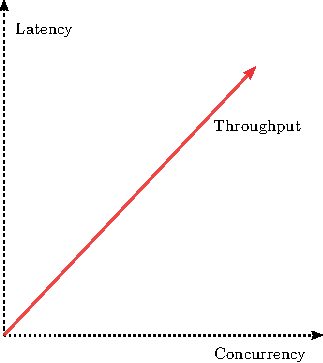
\includegraphics[width=0.35\paperwidth]{../figures/figure2.pdf}}}
    \qquad
    \subfloat[Scaling: read requests, write requests, or data]{{%
      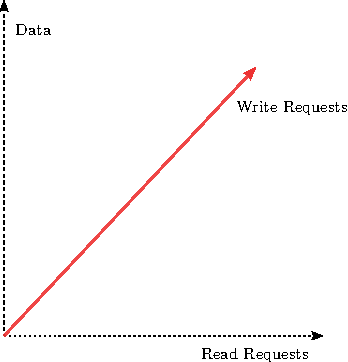
\includegraphics[width=0.35\paperwidth]{../figures/figure3.pdf}}}}
    \caption{Compromises of distributed systems\label{fig:compr}}
   \end{center}
\end{figure}

Keeping the above in mind, the benchmarks we have executed can be roughly
classified into four main categories, all of which having their own specific
goals.

The first category, aims to expose the effect in the job submission rate, when
the number of the master candidate nodes increases. In
order to effectively measure the overhead that is introduced with an increase in
the \texttt{candidate\_pool\_size} of the cluster, we will sent concurrently
\emph{errored} jobs to the master node, and then we will measure the rate that
Ganeti adds them to the queue. We intentionally chose to sent errored jobs,
because we simply want to observe how the job enqueue throughput of Ganeti
responds in various candidate pool sizes, and not any other factors that may be
affected by that type of measurement. The behavior we will observe, will also
indicate a suitable size of master candidate nodes, to conduct the rest of our
tests.

The second category, is a performance comparison test between the two driver
implementations; the default disk implementation that Ganeti currently uses, and
the CouchDB one. The comparison concentrates on the job submission rate, by
sending concurrently \emph{errored} jobs of various sizes similarly to the
previous category, but using a constant value of master candidate nodes instead,
the one that was determined previously. The aim is to measure the performance
against a tough workload, explain the differentiations, if any, that are
observed on both of the drivers, and expose the factors that have the greatest
impact on each of our drivers.

The third category deals solely with the configuration data management. We
measure the performance of the configuration related write requests, on several
file sizes, and in clusters with various candidate pool sizes, to examine the
bottlenecks on having a single configuration file on big production clusters
mainly. We will investigate all the factors that are delaying the update of the
configuration file, on both of the drivers, and then we conduct a comparison
test among them.

Lastly, in the forth benchmark category, we position the CouchDB and the disk
driver in a real-world scenario; an attempt to create a bunch of instances and
compare the total execution time of those jobs on each implementation. We aim to
present the overall performance of each driver, and explain any differentiations
that may arise.

\section{Evaluating CouchDB}\label{sec:perfom_couch}

The overview of the benchmark methodology we provided, points out the various
situations along with different metrics and workloads where we tested our
implementations, in order to measure accurately their performance. The
abovementioned categories, are presented in more details in the upcoming
sections.

\subsection{Impact of the candidate pool size}\label{subsec:cand_size}

This category is a sort of an introductory section for the rest of our tests.
Ganeti maintains a set of master candidate nodes, those that also contain a copy
of the full cluster configuration, i.e., configuration and jobs files. The
existence of those nodes has a great impact in the overall performance of the
cluster, due to the fact that each modification in a disk configuration file
causes a copy of it file to the candidate nodes. Creating a cluster with no
master candidates at all is a risky attempt, because in case of a master
failure all the cluster information will be lost. On contrast, maintaining a lot
of master candidate nodes is a redundant waste of resources, as modifications
have to be replicated to more nodes. We would ideally want to find out the set
of master candidate nodes that fits a production environment, in terms of having
the less impact in the cluster performance, and reducing the probability of a
cluster failure.

In order to decide which is the most appropriate candidate pool size, we
proceed with the following scenario. We sent jobs concurrently to Ganeti with
varying candidate node numbers, and we measure the rate in which jobs are
submitted to the queue, for each case.
This metric is the job enqueue throughput, and denotes the average number
of jobs that are added to the queue per second. It is a representative metric
for our purpose, because every new entry to the job queue will also be
replicated to the master candidate nodes before the operation is declared as
successful. Since we are just
interested for the enqueue rate, we decided to submit jobs that will
never be executed and will be declared as \emph{errored}. An example of those
jobs is the modification of an instance that does not exist in the cluster. The
jobs will be normally inserted to the queue and replicated to the candidate
nodes, but when they will start their execution, they will immediately fail as
\emph{errored}.

Jobs have been sent to Ganeti in batches of \texttt{10}, \texttt{20},
\texttt{30}, \texttt{40}, \texttt{50}, \texttt{100}, \texttt{150}, and
\texttt{200} jobs. We ran that benchmark in a \emph{5-node} cluster consisting
of \texttt{none},
\texttt{one}, \texttt{two}, and \texttt{four} master candidate nodes, and the
whole procedure has been repeated ten times in total. Since Ganeti writes every
information to filesystem and then distributes it to the candidate nodes, there
is a lot of disk and network I/O interaction. As a result, we expect a short of
deviation in our sample data values because there are external factors that may
affect the performance. The ``outliers" values that may arise should also be
included in the final results, because are part of the Ganeti behavior.
Consequently, we believe that the \emph{mean} value of our distribution is the
most appropriate metric for our case, because is a metric that represents the
\emph{central tendency} of the distribution by taking into account the whole
data information.

The benchmark outputs are summarized in two figures. Figure~\ref{fig:mc_comp},
presents the total results in a normal \emph{line-points} plot style, while
Figure~\ref{fig:const_jobs} concentrates on the heavier workload of our
benchmark that are closer to a real-world environment, in a clustered
\emph{bar-graph} plot.

\begin{figure}[htbp]
  \begin{center}
    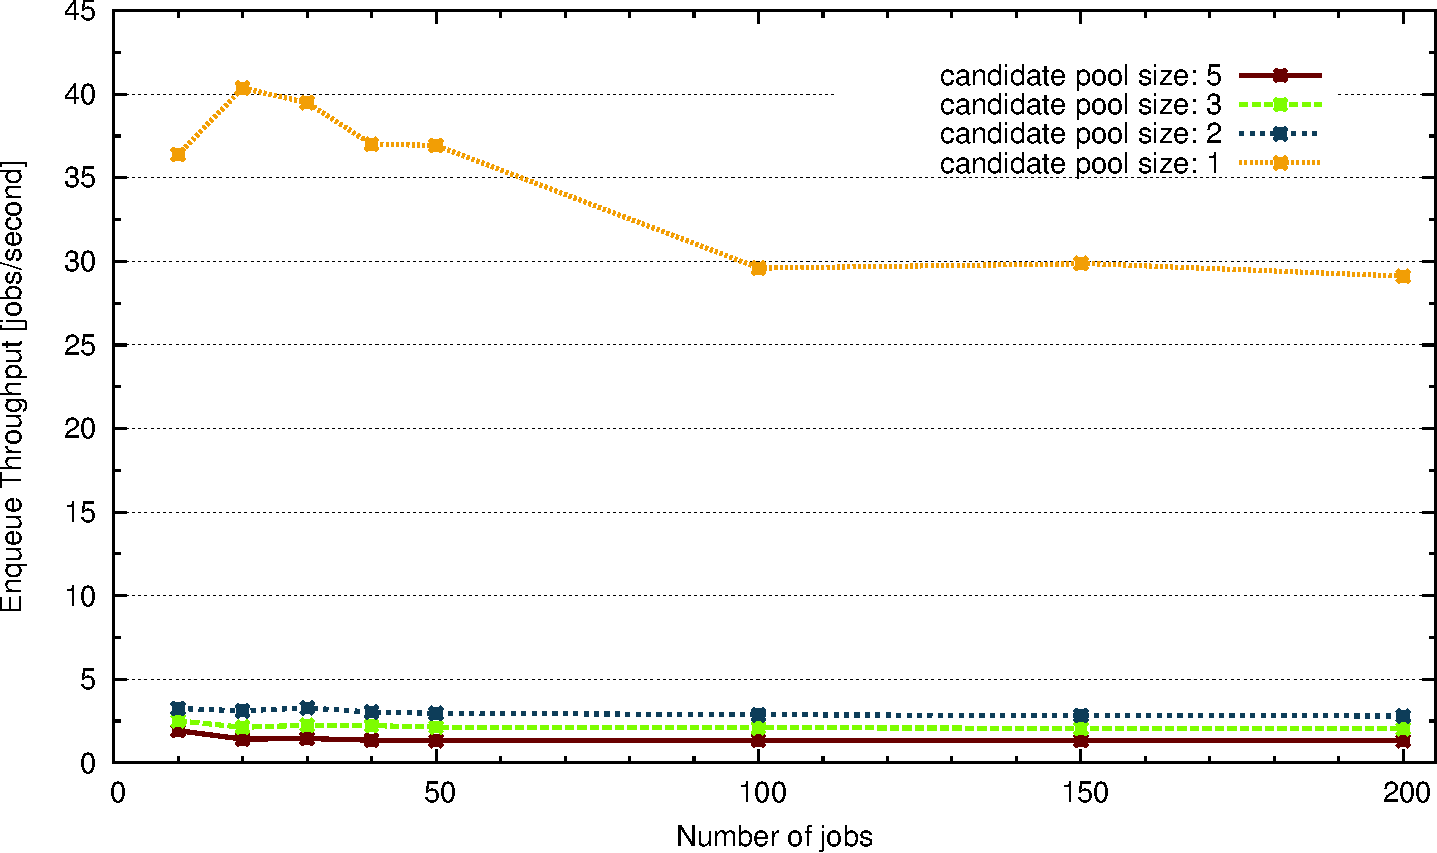
\includegraphics[width=1.0\maxwidth]{../figures/mc_comp.pdf}
    \caption{Job submission rate per number of candidates}
    \label{fig:mc_comp}
  \end{center}
\end{figure}

\begin{figure}[htbp]
  \begin{center}
    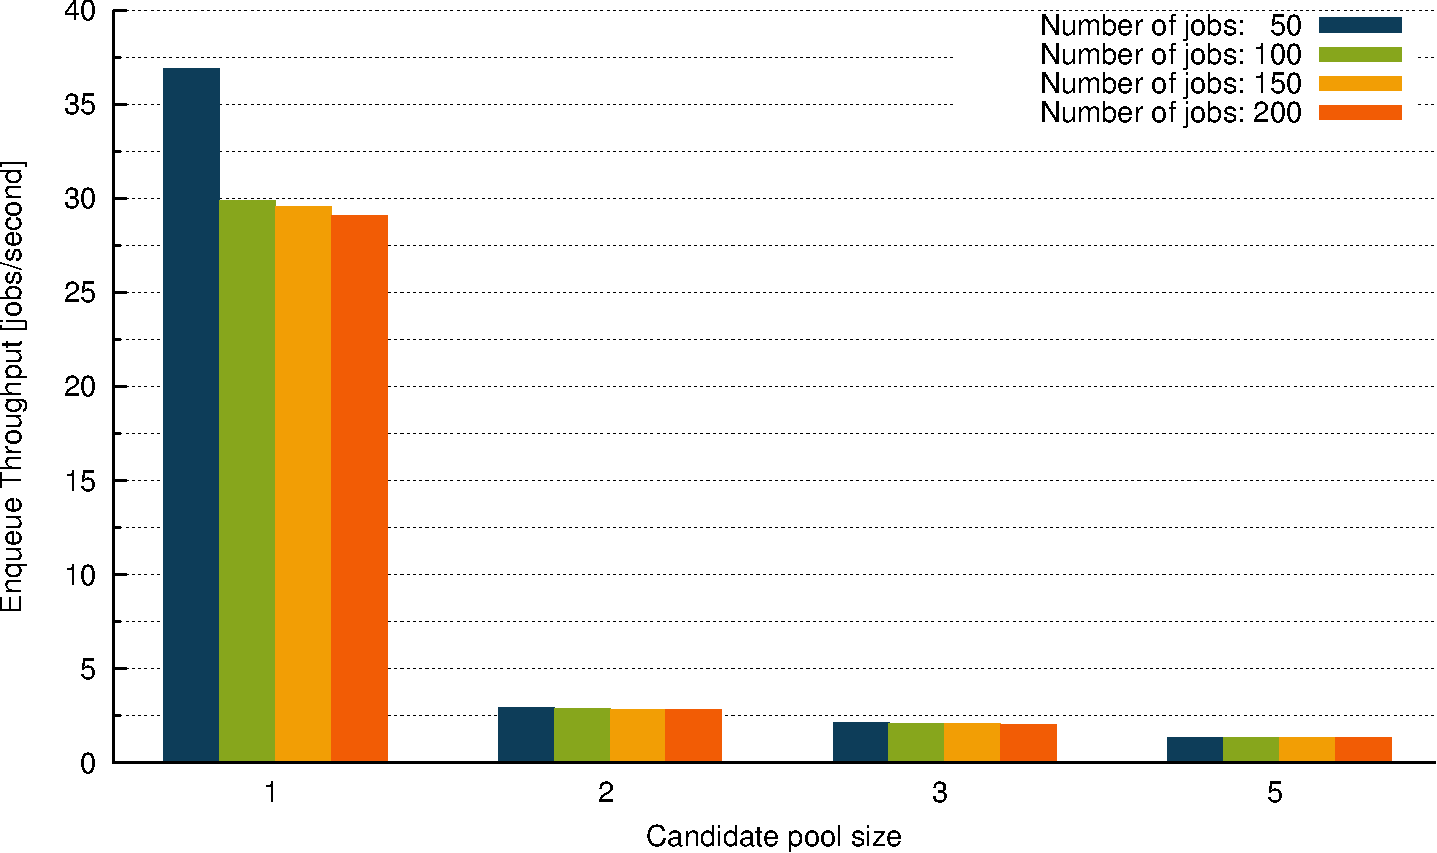
\includegraphics[width=1.0\maxwidth]{../figures/const_jobs.pdf}
    \caption{Job submission rate per number of candidates \#2}
    \label{fig:const_jobs}
  \end{center}
\end{figure}

\textbf{Performance Analysis}

There are several interesting points that we can conclude from these diagrams,
which we will address below. The most obvious observation is the significant
drop in the throughput performance, as we increase the master candidate
nodes of the cluster. Furthermore, in case of no master candidate nodes, the
distribution appears skewed characteristics and visible differentiations in the
throughput performance, something that is not observed when the candidate pool
size is increased. A closer explanation of those points follows.

In both figures, there is an obvious relationship between the job submission
rate and the number of master candidates that Ganeti maintains. As we stated in
the Caveats section, i.e., \ref{sec:caveats}, Ganeti writes jobs to disk and
then concurrently replicates them to the master candidates. The performance
slowdown of the replication process is displayed in these figures. With a single
master candidate node, we have a drop in the throughput of about \emph{8 times}
comparing to the case of no master candidates. An additional increase in the
candidate number, has no significant performance drop. This is an expected
behavior because Ganeti uses a multi-node RPC call to update the files in the
candidate nodes. This small dropdown is totally expected due to the checks that
Ganeti does after each RPC call, to get informed about the success, or not, of
the operation.

Another interesting finding from our results, are the ``outliers" that were
observed in the output sample data. When we ran the benchmarks in a cluster with
no master candidates, the data tended to have a more sparse behavior than in a
cluster with one, or more, candidate nodes. In order to make that variation
visible to the reader, we calculated the \emph{standard deviation} metric of our
distribution, which shows how much dispersion from the average value exists, and
we present it in Figure~\ref{fig:std} to justify our claim. The question that
may arise is: \emph{Why the deviation exists only in the case of a cluster with
no candidates}. The submission rate of Ganeti is the rate that the data are
written to disk, and replicated to the candidate nodes. Obviously, the disk and
network I/O are some of the factors that affect our results. As we know, Ganeti
writes the jobs to its queue, so when a worker thread grubs a job for execution,
it will subsequently update the job file in disk too. This causes
a lot of congestion in the job queue lock both from the master thread and the
job queue workers. The order that the workers grub jobs for execution causes
those differentiations in the throughput performance, in case of
no master candidates. On contrast, when the cluster contains master candidate
nodes, we have a totally smooth distribution with data around the mean value.
This behavior is justified by the replication process of the job files to the
candidate nodes. It is a quite time-consuming operation, that covers the
rest operations that are executed, and actually determines the result's form. At
this point, many types of measurements can be taken that will clarify those
claims and probably will expose more, but are out of the scope of this document
and this test category specifically, and we will not expand further.

\begin{figure}[htbp]
  \begin{center}
    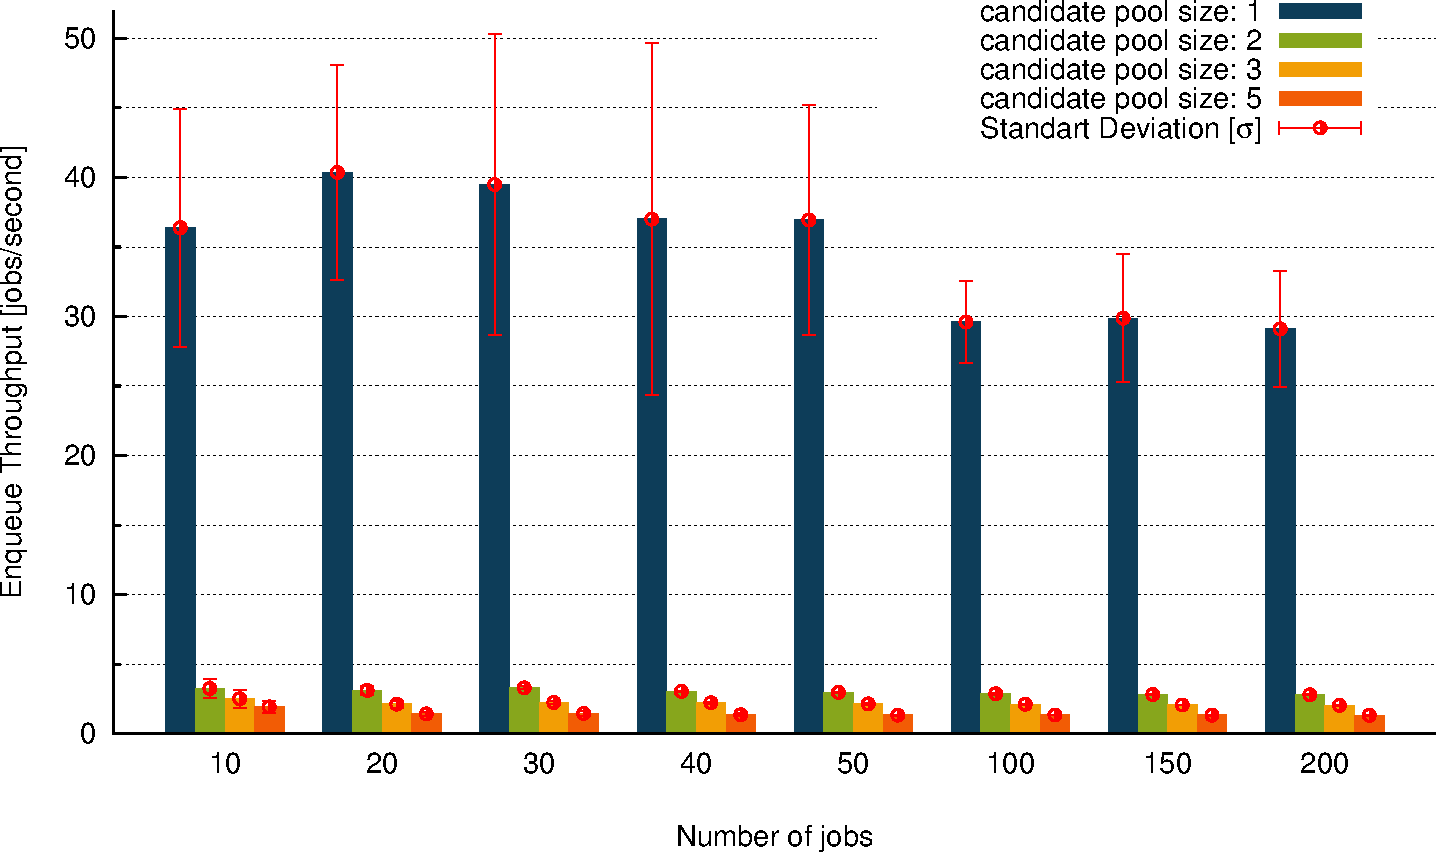
\includegraphics[width=1.0\maxwidth]{../figures/std.pdf}
    \caption{Standard Deviation [σ] of the job submission rate}
    \label{fig:std}
  \end{center}
\end{figure}

Summing up, from the results we presented, we believe that having a cluster with
two candidate nodes is the best choice to conduct the rest of our benchmarks. It
is also a choice that reflects a real production environment because it provides
the appropriate backup degree in case of a hardware failure, and also does not
have great performance impact comparing to a cluster with a single candidate
node.

\subsection{Comparison of the job submission rate}\label{subsec:enqueue_rate}

To some extend, we already discussed about the job submission performance rate
of Ganeti's default disk storage implementation, and we explained some of the
drawbacks that start to appear as the candidate pool size increases. In this
category, we make use of exactly the same metrics that we used in the previous
one, with the difference that the tests are conducted in a cluster with a
candidate pool size equal to \emph{three} nodes, as we determined in the first
benchmark category.

It is the first category where we actually compare the two driver
implementations, and we explain the main factors that affect their performance.
The results are summed up in two figures. Figure~\ref{fig:comp}, contains the
comparison of the job submission rate between CouchDB and the disk storage type,
while Figure~\ref{fig:couch_comp} presents the comparison of the CouchDB driver
performing under different socket options.

\begin{figure}[htbp]
  \begin{center}
    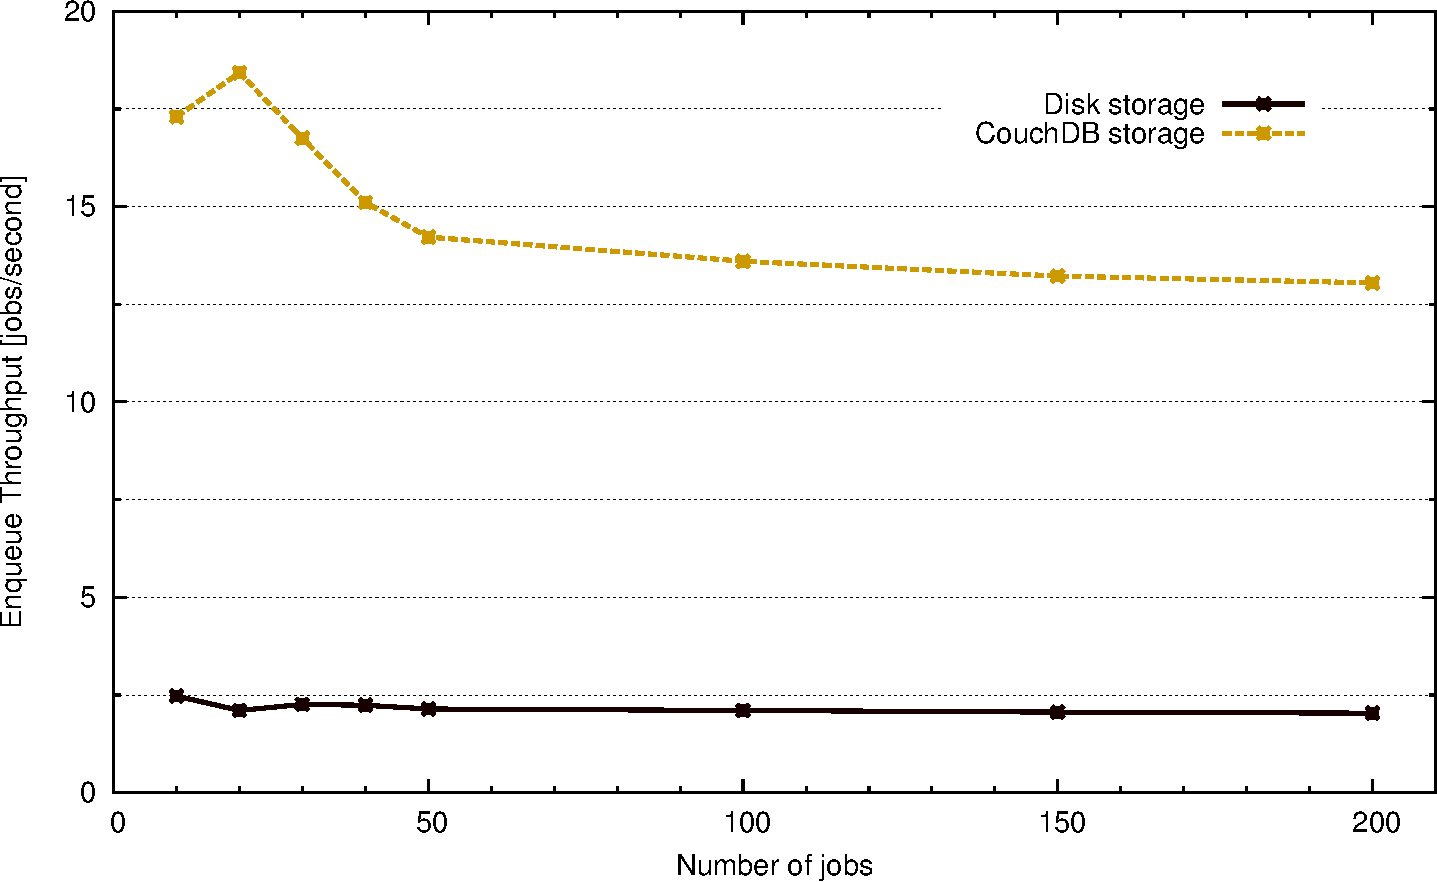
\includegraphics[width=1.0\maxwidth]{../figures/comp.pdf}
    \caption{Comparison of the throughput performance}
    \label{fig:comp}
  \end{center}
\end{figure}

\begin{figure}[htbp]
  \begin{center}
    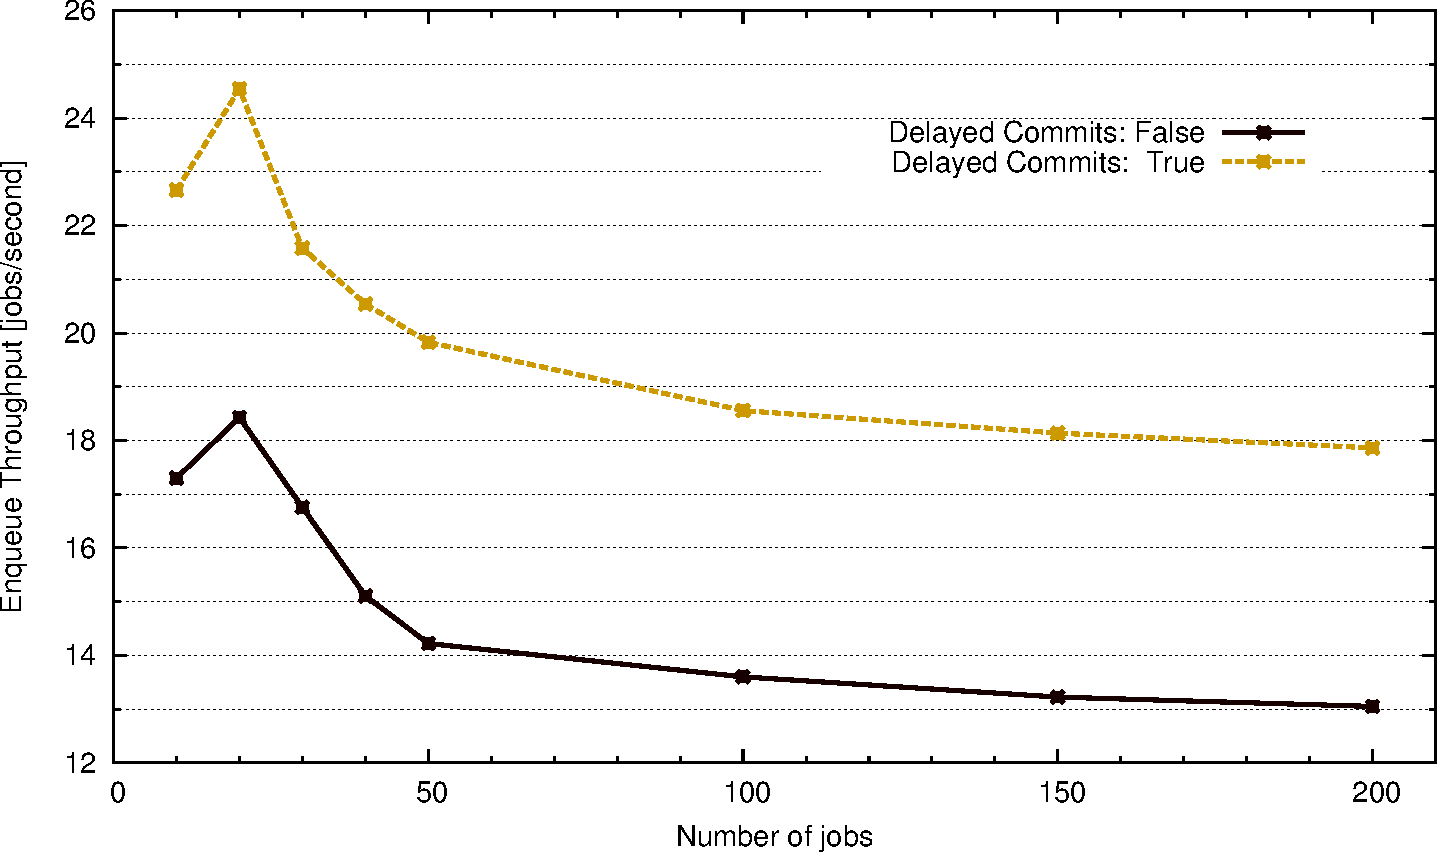
\includegraphics[width=1.0\maxwidth]{../figures/couch_comp.pdf}
    \caption{Throughput performance of CouchDB on various socket options}
    \label{fig:couch_comp}
  \end{center}
\end{figure}

\textbf{Performance Analysis}

Before we proceed with the interpretation of the diagram results, we have to
mention that the metrics we used, are exactly the same as in the first benchmark
category, and the final values correspond to the \emph{mean} value of every
distribution too.

Figure~\ref{fig:comp}, is the first performance comparison test that we
made between the two peers. The initial results look very promising. In a
\emph{5-node} cluster with two master candidate nodes, we have a speedup in the
job submission rate at about \emph{7-times} in the CouchDB driver, comparing to
the default disk storage implementation. The job submission rate has impact in
the overall job execution duration, as we will show in the last benchmark
category, and also reduces the timeouts happen in the LUXI server when many
clients try to submit jobs to Ganeti. We extensively talked about the reasons
that performance drops in a Ganeti cluster when jobs are saved to disk, in the
first test category. Now we are going to have a closer inspection in the
factors that prevent CouchDB from presenting similar behavior.

We discussed a lot about how Ganeti distributes the configuration files
to the candidate nodes, and we presented the performance impact of this
operation in the first category's figures. One of the main reasons we have
chosen CouchDB for Ganeti, is the replication feature, as it was discussed in
section~\ref{item:replication}. CouchDB is a database the replicates, and with
this term we mean that its fundamental function is to provide a simple, fast,
and convenient way to \emph{synchronize} two or more CouchDB databases.
Replication is handled completely by a separate process, external to Ganeti,
which listens on changes to the \emph{source} database, and replicates them to
the \emph{targets}. Obviously, the source refers to the master database, while
the targets are the databases of the candidate nodes. The \texttt{replicator}
process listens continually to the source's \texttt{\_changes} feed, and a new
modification to the source will immediately be replicated to the candidate
nodes. In order to ensure safety, CouchDB makes an \emph{fsync} call before a
\emph{201 Created} request is returned to the client. As soon as the
nodes are ``up" and running CouchDB will replicate, and there is no need to make
extra checks similar to the RPC checks that Ganeti has to make to find out that
the updates have reached a majority of the nodes, before declaring the
operation as successful. Instead, it is sufficient to check that the CouchDB
servers in the candidate nodes are accessible. This operation can be handled by
individual clients, independent to Ganeti that will not affect the performance,
and is an issue that is expected to be fixed in a future driver version, as we
will discuss in the Conclusion, i.e., Chapter~\ref{ch:conclusion}.

Besides the comparison test between the two implementations, we also make
a comparison test for the CouchDB drive,r on various socket options that CouchDB
provides, and have a great impact in the overall performance of the tool.
Figure~\ref{fig:couch_comp} shows this performance comparison test, on the
\texttt{delayed\_commits} attribute of CouchDB. When we set this attribute to
\texttt{True}, it is observed a further increase in the throughput performance
at about \emph{9-times} comparing to the default disk implementation, and at
about \emph{35\%} comparing to the CouchDB driver with this attribute set to
\texttt{False}. Delayed commits is probably the most important CouchDB
configuration setting for performance. When is set to true (the default),
CouchDB allows operations to be run against the disk without an explicit
\emph{fsync} call after each operation. Fsync operations take time in order to
complete, and calling them on each update limits the CouchDB performance for
sequential writers. It is clear that setting this option to true, opens a
window for data loss, because data are being kept in a write buffer and are
fsync-ed after a certain amount of time, or when the buffer is full. Ganeti is
an environment where we absolutely need to know when the updates have been
received, so we set this attribute to false, by default. The aim of this
test, is to expose an important setting of CouchDB that could be enabled
periodically, in several cases, like in a situation with an overloaded master
daemon, and then disabled at will. It is up to the cluster administrator to
measure the tradeoff between loosing some data in case of a hardware failure,
and the ``relief" that the performance improvement will bring to the cluster.

To achieve the results we presented for the CouchDB driver, another
important configuration option must be modified, related to the TCP buffering
behavior. This is the \emph{nodelay} option which must be set to \texttt{True},
in order to disable the \emph{Nagle's algorithm}~\flink{http://en.wikipedia.org/
wiki/Nagle\%27s\_algorithm}, which introduces an additional delay when using
keep-alive HTTP-connections. By setting this option to true, the
\emph{TCP\_NODELAY} option is turned on for socket, which means that even small
amounts of data sent to the TCP socket, like the reply to a document write
request, or reading a very small document, will be sent immediately to the
network. They will not be buffered hoping that it will be asked to send more
data through the same socket in order to transfer them all at once. The main
reason that this important option is disabled by default, is that the last
releases of CouchDB ships with a more recent version of the HTTP server library
\emph{MochiWeb}~\flink{https://github.com/mochi/mochiweb}, which by default sets
the \emph{TCP\_NODELAY} socket option to false.

\subsection{Comparison of the config.data performance}\label{subsec:config_perf}

The CouchDB driver, besides the alternative storage solution that provides to
the configuration files of Ganeti, also introduces a variation in the
way it handles the \texttt{config.data} file, as it was extensively discussed
in Section~\ref{sec:config}. The ultimate aim of this category is to compare the
performance of the two alternative implementations of handling the configuration
file, but before we reach to this point, we will investigate in deep all the
factors that affect the configuration file performance, and that were discussed
in Section~\ref{sec:caveats}.

In this category we will present three diagrams in total. The first two
of them [\ref{fig:total-cfg}, \ref{fig:couchdb}], one for each driver,
show the total execution duration of the \texttt{\_WriteConfig} method, and all
the sub-method calls that are been made. This is the responsible method for
applying the changes of the configuration file to the permanent storage, and
replicate them to the master candidate nodes.
Every operation that modifies the cluster state calls this function to
make the changes permanent. It is the most time consuming function related to
the configuration file, and has a great importance in the performance of Ganeti,
because is must be called with the \texttt{ConfigWriter} lock held in exclusive
mode, which starts to become a bottleneck when a huge number of jobs is in
execution. If we manage to reduce the time the lock is held by the workers, we
will also reduce some of the congestion in the config lock. The last diagram
[\ref{fig:comp-cfg}], is the actual performance comparison plot between the two
implementations.

The benchmarks of this section have been conducted on a cluster with a candidate
pool size equal to \texttt{one}, \texttt{three}, and \texttt{five} nodes,
respectively. In order to measure the performance of the \texttt{\_WriteConfig}
method, we intentionally increased the size of the \texttt{config.data} file,
from \texttt{100 KB} up to \texttt{5 MB}. A cluster with about \emph{2.000}
instances has a configuration file of around \texttt{5 MB}, which corresponds to
a real workload for a production environment. Our test concentrates on modifying
a parameter of a single configuration object. We chose an instance object as a
use case. Starting, restarting, or stopping an instance is a quite commonly used
operation, that while it aims to modify a single field of the instance object,
the whole configuration object is flushed to disk, and moreover the
\texttt{ssconf\_*} files are not affected; a variance that we do not want
to take into account in this test category. The test was repeated \emph{20}
times for each pair, and we find it appropriate to make use of the
\emph{trimmed mean} value of our distribution. The trimmed mean is a method of
averaging, that removes a small percentage of the largest and the smallest
values before calculating the mean. This method aims to reduce the effects of
the outliers on the calculated average, and stated as mean trimmed by
\emph{X\%}, where \emph{X} is the sum of the percentage of observations
removed from both the upper and lower bounds. In our case, we trimmed the mean
by \emph{20\%}. The reason we did not calculate the normal mean value, is that
we wanted to reduce the effects of the outliers that were observed, and to
obtain a more accurate average performance overview, for both the
implementations.

\bigskip
\textbf{Performance Analysis}

In the begging of our analysis, we will take a closer inspection on all the
factors related to the performance of the write operation of the
configuration file. An operation that affects the configuration state, passes
from the following execution phases in general. Firstly, some preliminary checks
are being made on the object that it is requested to change, and then the
update of the in-memory representation of the \texttt{config.data} object
follows. Then the \texttt{\_WriteConfig} method is called, which flushes the
updates to disk, and replicates them to the candidate nodes. This method
consists of a number
of time-consuming sub-method calls that affect the overall performance of any
cluster operation that modifies the configuration file. These calls contain the
verification of the config object for configuration errors, to maintain the
consistency of the object, and is named \texttt{\_UnlockedVerifyConfig}, the
serialization of the config object in order to be prepared for applying the
changes to disk, through the \texttt{serializer.Dump} call, and then the actual
flushing of the in-memory object to disk, using the \texttt{utils.SafeWriteFile}
function call. Finally, the modifications have to be replicated to the candidate
nodes with the \texttt{\_DistributeConfig} method. All these operations are
affected from the size of the configuration file, and from the candidate pool
size as well. Figure~\ref{fig:total-cfg}, extensively examines this behavior.

From Figure~\ref{fig:total-cfg}, the following conclusions can be made. The most
time-consuming method, is the serialization of the configuration file. It
is a totally independent cost from the candidate pool size, but it is 100\%
bounded with the size of the file. The file is stored in
memory as a \texttt{ConfigData} object, a generic config object defined by
Ganeti. In order to be saved to disk, it must be transformed to a string format,
and this is the role of this method. The cost of the file replication to the
candidate nodes is increases along with the number of master candidates, and the
size of the file too. In the same sense, the verification check consumes a lot
of time in bigger file sizes because it traverses the whole file, same as the
time of the function that applies the changes to disk, but with the difference
that even in bigger file sizes it
does not consume a noticeable amount of time. From this diagram it is understood
that in a cluster with three candidate nodes, even from a file of \emph{1.0 MB}
in size, it takes at about \emph{1 sec} to complete a single operation.
If we combine it with the congestion on the config lock, we can see
the great impact of that delay in the overall cluster's performance.

It is obvious that a single configuration file comes with a number of
disadvantages. Modifying a single field of the file requires the serialization
of the whole config object and the distribution to the candidates, as well. This
approach reduces the cluster performance due to the increased operational cost
that is implied. In Figure~\ref{fig:couchdb}, we will present a different
approach that the CouchDB driver introduces, by conducting the same test on the
\texttt{\_WriteConfig} method of the CouchDB driver.

In Figure~\ref{fig:couchdb}, we observe a great improvement in the total
execution duration of updating the configuration file. This differentiation can
be justified by the different approach of CouchDB of handling the config object.
The configuration file has been separated to its sub-components, as
we extensively discussed in section~\ref{item:config}. Modifying an instance, a
node, and generally a single object of the configuration file, does not updates
the whole object to disk, but only the single object we want to.
Moreover, the serialization cost does not
implies anymore. The transformation of an object before it is written to disk
is a simple conversion to dictionary, and it is part of the
\texttt{utils.WriteDocument} method. Since we convert only few kilobytes each
time the cost is negligible. The distribution cost is also disappears due to
the different approach of CouchDB on handling the replication process, as we
already extensively explained. The verification cost is the only one that does
not changes, since we continue to verify the whole in-memory configuration
object.

The last diagram we are going to present in this category, is presented in
Figure~\ref{fig:comp-cfg}. It displays the total execution duration of an
instance modify operation. It is a representative job, as all Ganeti operations
modify a specific field of the configuration file. The same output would appear
if we were modifying a node, a network, or a nodegroup. As we said in the
\emph{Implementation Details} section of the CouchDB driver, i.e., Section
\ref{sec:couch_details}, every update causes two consecutive object updates to
the CouchDB server. One for the cluster general information, and one for the
object we want to change. In this figure, we present the total execution time
for CouchDB, that is the aggregated execution duration of the two objects.
Even with this overhead the difference of flushing the whole file to disk
comparing to the single object that is updated is significant. For example, for
a file of \emph{2 MB} in size, we have at about \emph{5-times} increase in the
performance of CouchDB, while the gap is widening as the file size further
increases.

\begin{figure}[htbp]
  \begin{center}
    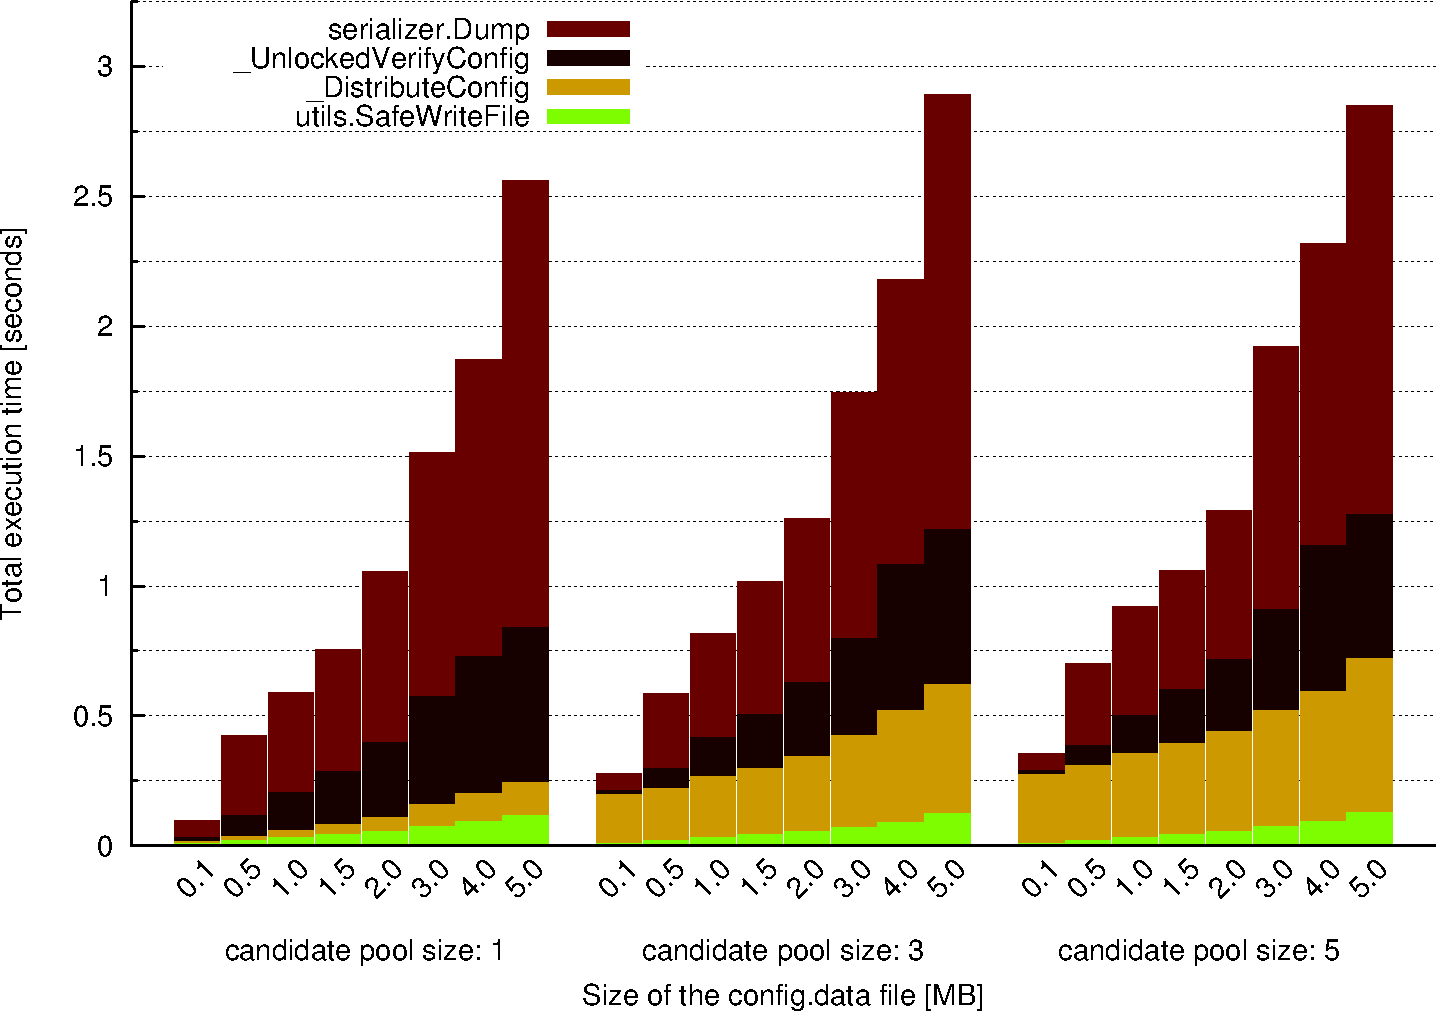
\includegraphics[width=1.0\maxwidth]{../figures/total-cfg.pdf}
    \caption{Performance evaluation of the default \_WriteConfig method}
    \label{fig:total-cfg}
  \end{center}
\end{figure}

\begin{figure}[htbp]
  \begin{center}
    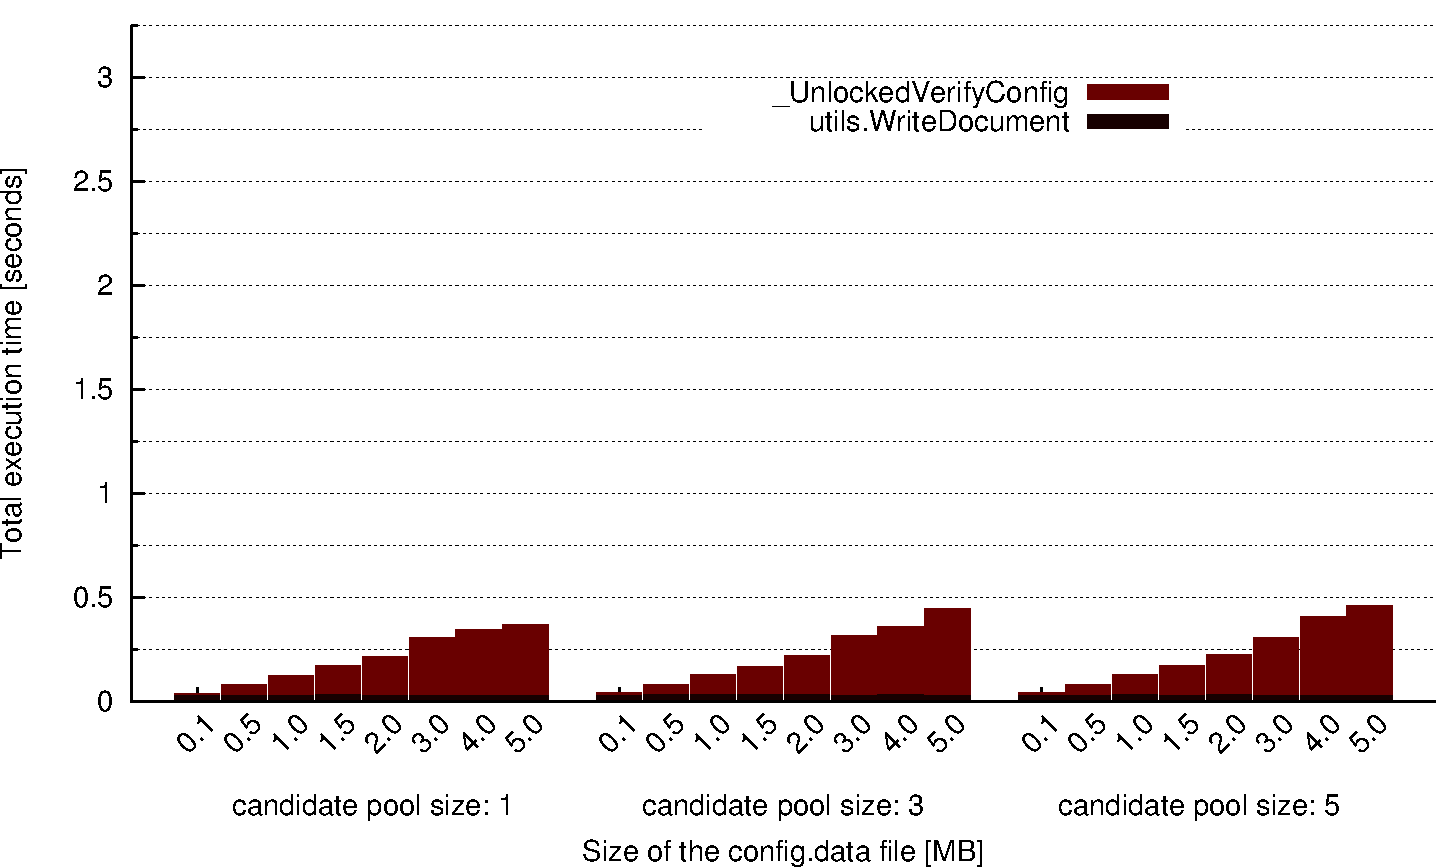
\includegraphics[width=1.0\maxwidth]{../figures/couchdb.pdf}
    \caption{Performance evaluation of the \_WriteConfig method of CouchDB}
    \label{fig:couchdb}
  \end{center}
\end{figure}

\begin{figure}[htbp]
  \begin{center}
    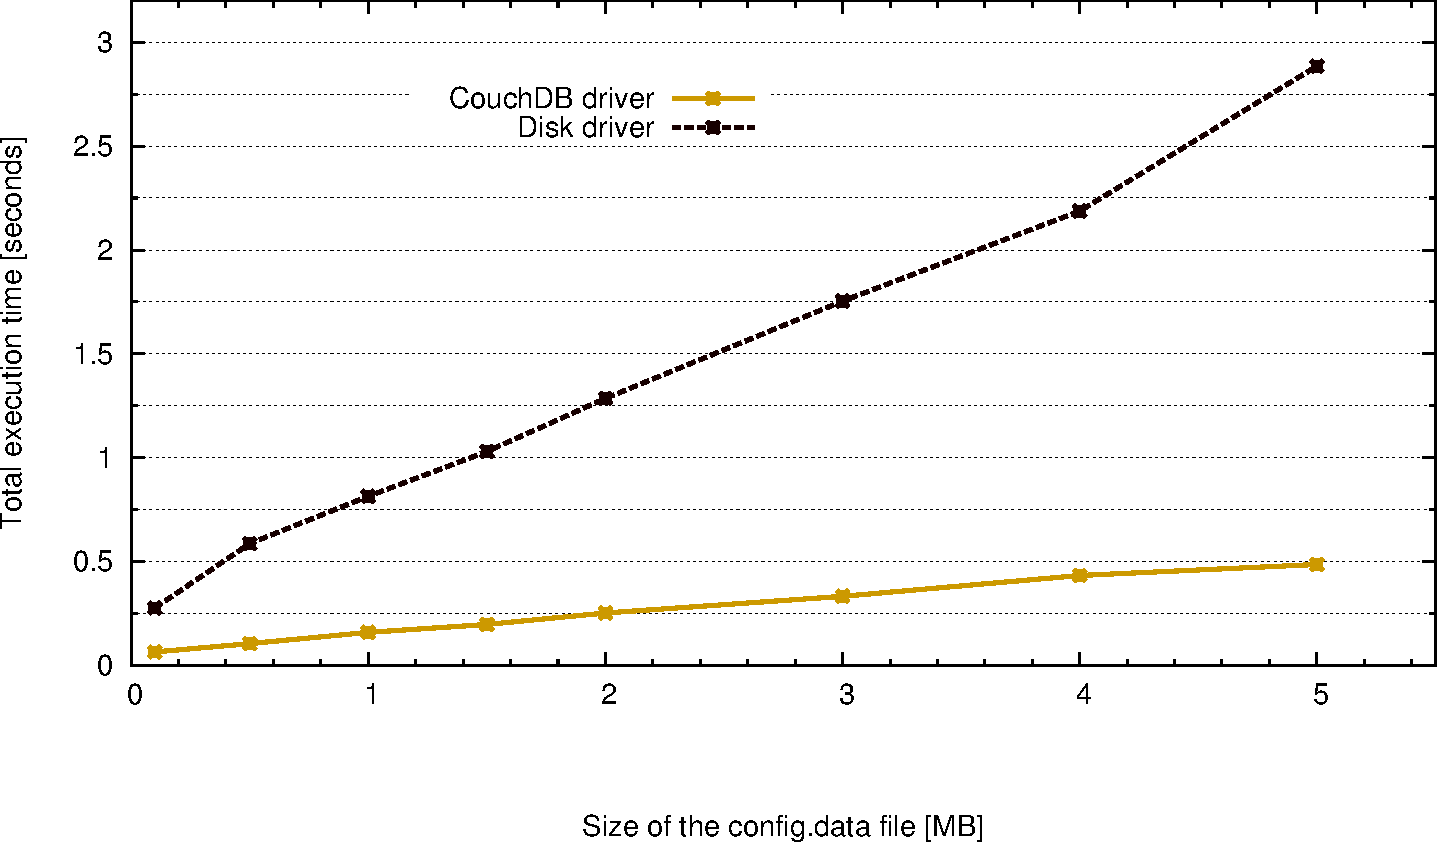
\includegraphics[width=1.0\maxwidth]{../figures/comp-cfg.pdf}
    \caption{Comparison of execution performance for instance modify ops}
    \label{fig:comp-cfg}
  \end{center}
\end{figure}

\subsection{Aggregate evaluation of the CouchDB driver}\label{subsec:total_eval}

Up to this point, we have tested our implementation in a variety of situations
that may occur in a Ganeti cluster. We also examined some of the main factors
that limit Ganeti from scaling and achieving better performance. In this last
benchmark category, we will attempt to measure the overall performance of
our drivers in a real-world scenario. In order to explain the results of this
section, we will also make use of the findings from the previous categories.

In a Ganeti cluster with \emph{5 vm-capable} nodes, and three master candidates,
we will concurrently submit jobs of \emph{OpInstanceCreate} opcodes, in batches
of \texttt{1}, \texttt{10}, \texttt{20}, \texttt{50}, and \texttt{100} jobs. We
will measure the average time of the phases that a job passes through, and then
the total execution duration from the first job that it is enqueued since the
last that is completed. Since the \texttt{Running} times of the jobs are
independent to the underlying storage layer that it is used, we will minimize
it by creating instances with \emph{1 GB} file disk, using the
\emph{--no-install}, \emph{--no-start} options that disable the OS installation
and the start-up of the instances respectively.

\bigskip
\newpage
\textbf{Performance Analysis}

Figure~\ref{fig:jobs_avg}, displays the average duration of the execution phases
of the \emph{InstanceCreate} jobs we submitted. For a short reminder about the
execution phases of a job, refer to Section~\ref{subsec:jobs}.

\begin{figure}[htbp]
  \begin{center}
    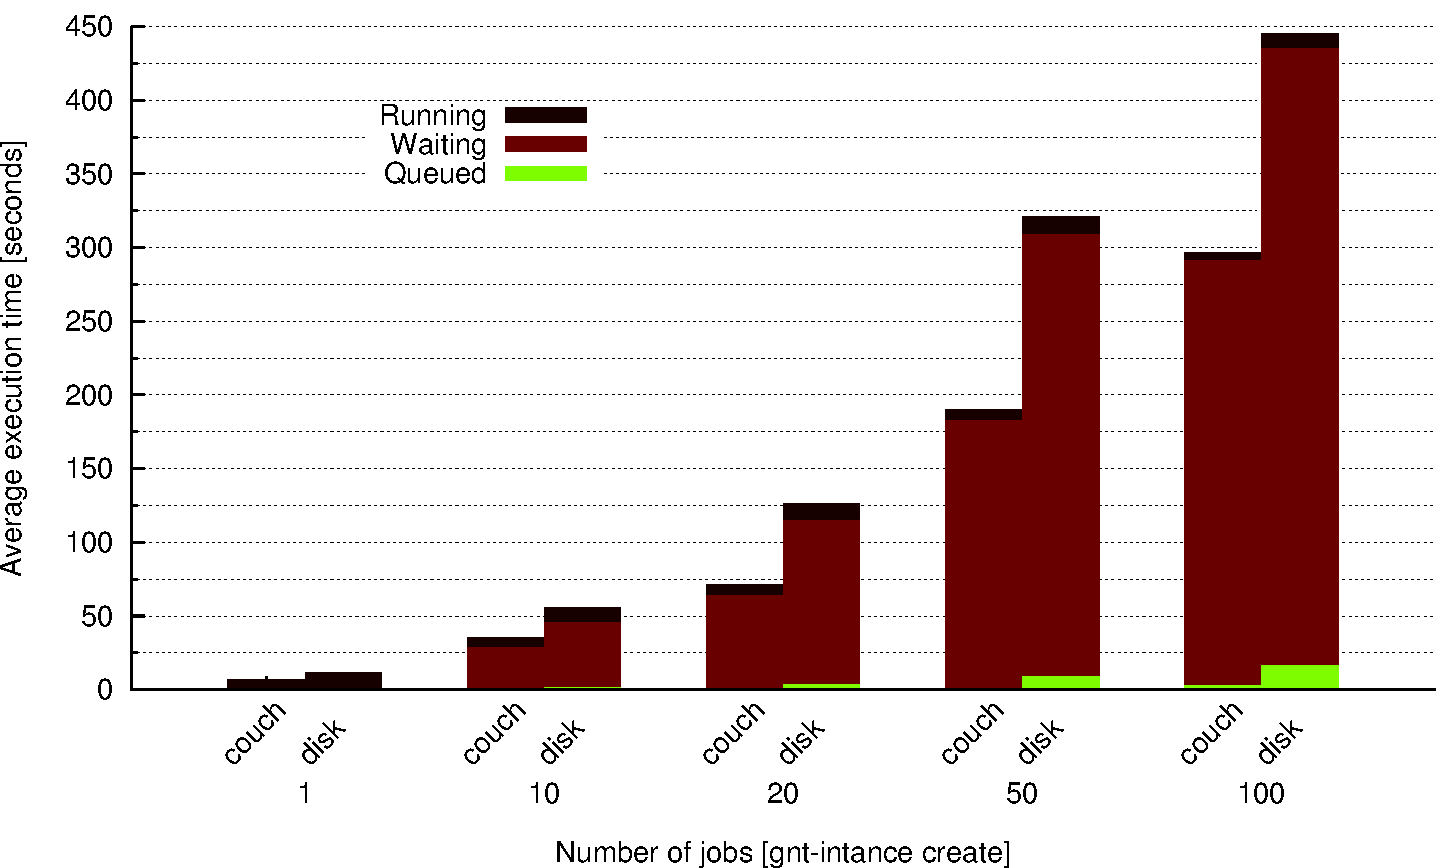
\includegraphics[width=1.0\maxwidth]{../figures/jobs_avg.pdf}
    \caption{Comparison of execution performance for the phases of a job}
    \label{fig:jobs_avg}
  \end{center}
\end{figure}

What we observe from Figure~\ref{fig:jobs_avg}, is a minimized \emph{Running}
time for reasons we already covered, while the most time is consumed in the
\emph{Waiting} phase. In this phase the jobs are waiting for locks, held by other
threads that are in execution. The \emph{Opportunistic locking} that it is used
since Ganeti version \emph{2.7}, improved the lock congestion in instance create
operations, but since we create a lot of instances in a small cluster, it is a
normal behavior. It is also observed that the average time of CouchDB in the
\emph{Queued}, and \emph{Waiting} phase is quite smaller comparing to the disk
implementation. We already covered the improved performance in the submission
rate of CouchDB. The new finding, is the increase in the average \emph{Waiting}
performance time. This behavior can be justified by the increased job submission
rate, as we presented in Figure~\ref{fig:comp}. The worker threads, are waiting
in the queue for new jobs to appear. As soon as a job is submitted in the queue,
and a worker thread is available, it grubs it for execution. An increased job
enqueue rate translates to workers that acquire their workload earlier. As a
result, we have an immediate impact in the \emph{Waiting} average time, due to
the fact that the workers are idle for less time than they previously were, and
the resources of the cluster are exploited more efficient than before. An
immediate consequence of the increase in the performance of the \emph{Queued}
and \emph{Waiting} time, is an increase in the total execution duration of the
jobs. This induction is justified by~Figure~\ref{fig:total_secs}.

\begin{figure}[htbp]
  \begin{center}
    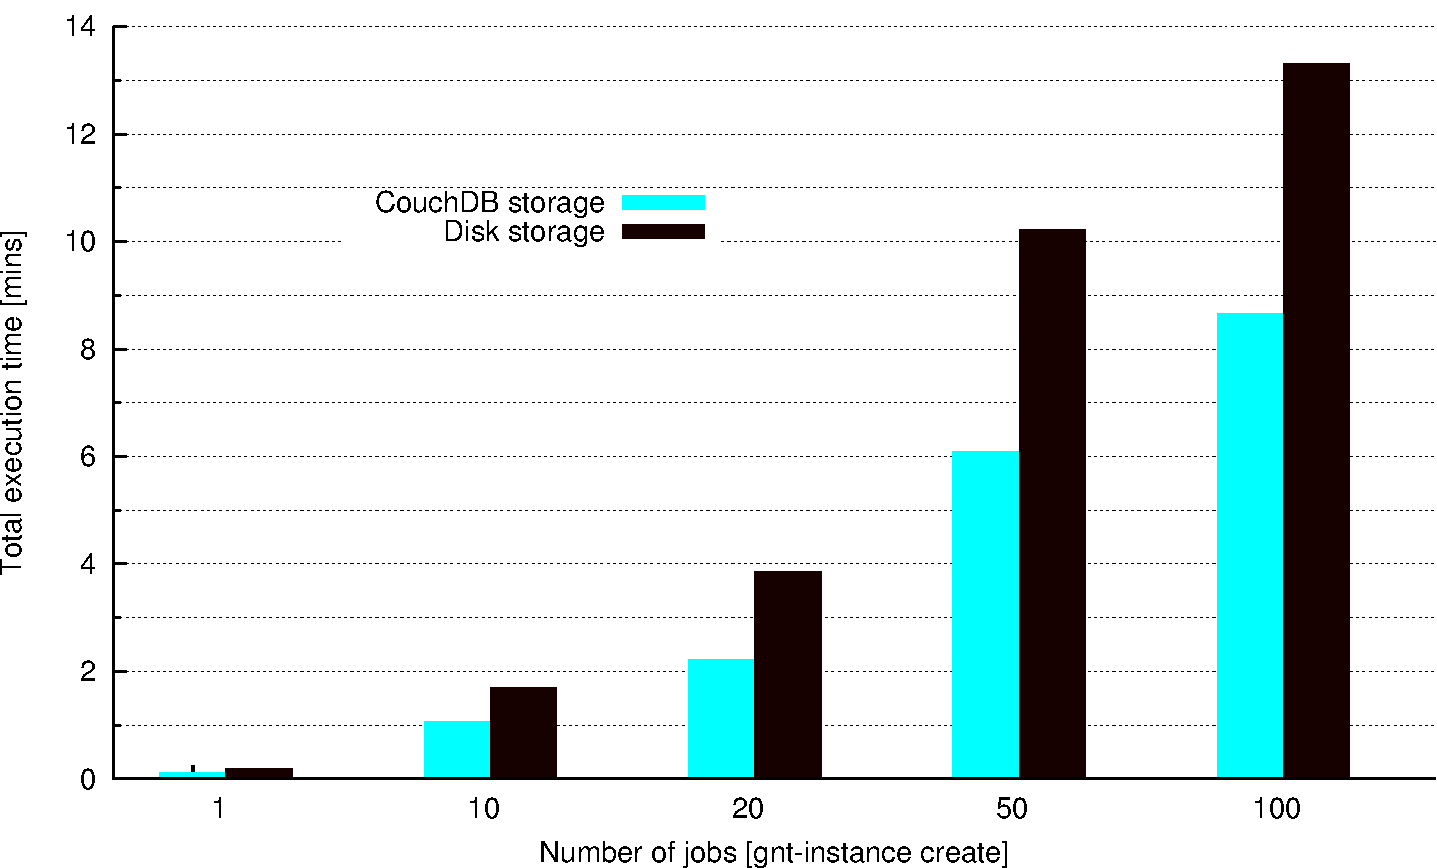
\includegraphics[width=1.0\maxwidth]{../figures/total_secs.pdf}
    \caption{Comparison of the throughput performance for instance create ops}
    \label{fig:total_secs}
  \end{center}
\end{figure}

What we conclude from Figure~\ref{fig:total_secs}, is that the CouchDB driver
performs better under a heavy loaded environment. The performance gap between
the two implementations widens as the number of jobs in the cluster increases.
CouchDB is designed to service highly concurrent use cases, and perform under a
heavy application load. The \emph{Multi-Version Concurrency Control} that
implements, makes CouchDB able to handle a high volume of concurrent readers and
writers without conflicts to each other. As a result, there will not appear any
performance gaps as the cluster workload is increased, and the requests will
continue to be serviced efficiently.

\chapter{Performance Evaluation}\label{ch:performance}

In this Chapter, we will evaluate the performance of the new CouchDB driver
comparing to the default disk implementation, that is currently used by Ganeti
for its storage requirements. Good benchmarks are non-trivial; each driver is
different, and different use cases need to tune different parameters. In next
sections, we will try to illustrate the benchmarking methodology of the diagrams
we are about to present, before we proceed to the detailed explanation of our
results.

The structure of this chapter is the following. Section~\ref{sec:specs} provides
details about the hardware and software on which we conducted our benchmarks,
while section~\ref{sec:bench} concentrates on the methodology behind our
measurements; the main factors we have taken into account in order to
decide which were the most interesting and applicable for Ganeti fields, were we
should evaluate our driver's performance. Finally, section
\ref{sec:perfom_couch} contains the actual performance evaluation of the CouchDB
driver. In each of its subsections concentrates on a specific field of interest
for the driver evaluation, which will subsequently lead us to the final
conjecture about how the driver responds to real-world workloads.

\section{Specifications}\label{sec:specs}

To evaluate our software tool, it was required to setup a Ganeti
cluster where our benchmarks would run. We decided to setup our testing cluster
into a virtualized environment. More specifically, we chosen \emph{Synnefo}
\flink{http://www.synnefo.org/}, an open source cloud software, to host our
testing environment. A bunch of reasons lead us to this decision. Firstly, as
Ganeti is a software tool for managing clusters of physical nodes, it is not a
facile task to obtain, setup, and maintain physical machines for the cluster
requirements. On contrast, using a virtualized environment makes it quite easy
to add and remove nodes from the cluster at will, without interacting with any
physical processes that would be running in a physical machine. It
provides a complete isolated environment where no one else can intervene with
our work. In addition, keeping up-to-date snapshots of our virtual nodes makes
disaster recovery quite a bit easier, and our cluster can be recovered in just a
few seconds in case of a hardware or a software failure. Moreover, it makes
incredibly simple and fast to modify the underlying hardware we use for our VMs,
through the hardware abstraction it is provided.

On the contrary, every virtualization solution comes with an additional overhead
in terms of computation, networking, and I/O operations. The overhead incurred
by virtualization has been the focus of many performance studies in the past,
including numerous of general-purpose benchmarks. A short review on those,
indicates an overhead below \emph{5\%} on computation~\cite{xen_art}, below
\emph{15\%} on networking~\cite{xen_art, diagnosing}, while the parallel I/O
performance losses  due to virtualization has been shown to be below
\emph{30\%}~\cite{xen_hpc}, respectively. Recently, there also has been occurred
a burst on the research activity related to the performance of using virtualized
resources in cloud computing environments~\cite{montage, Iosup_anearly,
parallel}, that provide additional metrics of the effects of using the cloud
computing services for running many types of scientific tasks.

In our case, the testing environment has been setup in a \emph{7-node}
cluster, where each node was armed with a \emph{24-core AMD Opteron(tm) 6172}
processor at \emph{2.10 GHz}, with \emph{189 GB} of primary memory, and
\emph{3.7 TB} of storage, running on a \emph{SMP Debian GNU/Linux} with
\emph{3.2.0-4} kernel in \emph{64-bit} mode. The virtualization software used,
was \emph{QEMU 1.7.0} with the aid of the \emph{KVM} kernel module. When used as
a virtualizer, QEMU achieves near native performance by executing the guest code
directly on the host CPU. The redundancy on the physical resources of the
nodes we setup our cluster, provides 1:1 mapping between the CPUs and vCPUS, as
for the primary memory too. This results to a
minimum performance overhead because there is no overcommitment in the physical
resources at all. On the contrary, we can not come through the overhead during
I/O operations with the disk and the network usage, but keeping in mind that both
of our drivers interact with the disk and make use of the network resources,
that overhead is linearly applied to each of them and will not affect the final
results. The specifications of each one of the VMs constituting our virtual
\emph{5-node} Ganeti cluster, where we conducted our benchmarks, are the
following.

\begin{table}[htbp]
  \centering
  \begin{tabular}{ | l | l | }
    \hline
    Component & Description \\ \hline \hline
    CPU & 8 x QEMU Virtual CPU Version 1.7.0 \\
    \hline
    RAΜ & 8192 MB  \\
    \hline
    Disk & 80 GB \\
    \hline
  \end{tabular}
  \caption{Test-VM hardware specs}
  \label{tab:hw-specs}
\end{table}

\begin{table}[htbp]
  \centering
  \begin{tabular}{ | l | l | }
    \hline
    Software & Version \\ \hline \hline
    OS & Debian 7.1 Wheezy Base System \\
    \hline
    Linux Kernel & 3.2.0-4-amd64  \\
    \hline
  \end{tabular}
  \caption{Test-VM software specs}
  \label{tab:soft-specs}
\end{table}

\section{Benchmark methodology}\label{sec:bench}

Real benchmarks require real-world load. We will try to test our driver on
real-world examples under situations when hundreds of clients try to interact
with the master daemon concurrently, meaning that the masterd has to deal with
them properly. Ganeti is a distributed software tool. So it is a premise to
scale well and perform-fast, when used in real production environments with tens
of nodes on each cluster.

There are a plenty of attributes affecting the performance of distributed
systems and multiple ``knobs" we could turn on to make a system perform better
in one area, but affecting another area when doing so. A use case is the CAP
theorem that was discussed in section~\ref{item:cap}. If we want our system to
scale out, for example, there are three distinct areas to deal with; increased
read and write requests, and data. In addition, reducing latency for a given
system, affects concurrency and throughput capabilities. These two examples are
graphically illustrated in Figure~\ref{fig:compr}.
Orthogonal to those attributes, there are many more factors that affect a system
such as Ganeti, and more of the figures below can be drawed, that display
different features such as reliability, simplicity, availability, and more.
CouchDB is very flexible and gives us enough tools to create a system shaped to
suit many, \underline{but not all}, of our problems.

\begin{figure}[htbp]
  \begin{center}
    \makebox[\textwidth]{%
    \subfloat[Performance: Throughput, latency, or concurrency]{{%
      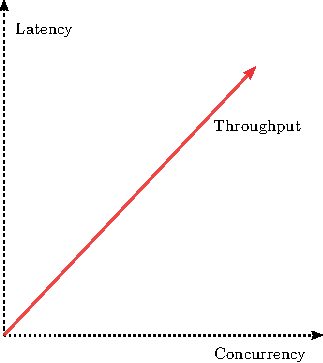
\includegraphics[width=0.35\paperwidth]{../figures/figure2.pdf}}}
    \qquad
    \subfloat[Scaling: read requests, write requests, or data]{{%
      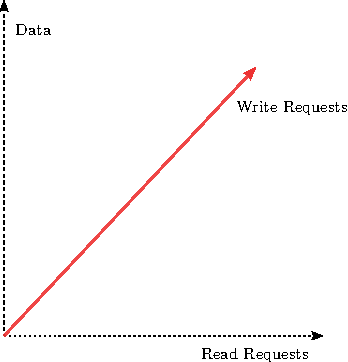
\includegraphics[width=0.35\paperwidth]{../figures/figure3.pdf}}}}
    \caption{Compromises of distributed systems\label{fig:compr}}
   \end{center}
\end{figure}

Keeping the above in mind, the benchmarks we have executed can be roughly
classified into four main categories, all of which having their own specific
goals.

The first category, aims to expose the effect in the job submission rate, when
the number of the master candidate nodes increases. In
order to effectively measure the overhead that is introduced with an increase in
the \texttt{candidate\_pool\_size} of the cluster, we will sent concurrently
\emph{errored} jobs to the master node, and then we will measure the rate that
Ganeti adds them to the queue. We intentionally chose to sent errored jobs,
because we simply want to observe how the job enqueue throughput of Ganeti
responds in various candidate pool sizes, and not any other factors that may be
affected by that type of measurement. The behavior we will observe, will also
indicate a suitable size of master candidate nodes, to conduct the rest of our
tests.

The second category, is a performance comparison test between the two driver
implementations; the default disk implementation that Ganeti currently uses, and
the CouchDB one. The comparison concentrates on the job submission rate, by
sending concurrently \emph{errored} jobs of various sizes similarly to the
previous category, but using a constant value of master candidate nodes instead,
the one that was determined previously. The aim is to measure the performance
against a tough workload, explain the differentiations, if any, that are
observed on both of the drivers, and expose the factors that have the greatest
impact on each of our drivers.

The third category deals solely with the configuration data management. We
measure the performance of the configuration related write requests, on several
file sizes, and in clusters with various candidate pool sizes, to examine the
bottlenecks on having a single configuration file on big production clusters
mainly. We will investigate all the factors that are delaying the update of the
configuration file, on both of the drivers, and then we conduct a comparison
test among them.

Lastly, in the forth benchmark category, we position the CouchDB and the disk
driver in a real-world scenario; an attempt to create a bunch of instances and
compare the total execution time of those jobs on each implementation. We aim to
present the overall performance of each driver, and explain any differentiations
that may arise.

\section{Evaluating CouchDB}\label{sec:perfom_couch}

The overview of the benchmark methodology we provided, points out the various
situations along with different metrics and workloads where we tested our
implementations, in order to measure accurately their performance. The
abovementioned categories, are presented in more details in the upcoming
sections.

\subsection{Impact of the candidate pool size}\label{subsec:cand_size}

This category is a sort of an introductory section for the rest of our tests.
Ganeti maintains a set of master candidate nodes, those that also contain a copy
of the full cluster configuration, i.e., configuration and jobs files. The
existence of those nodes has a great impact in the overall performance of the
cluster, due to the fact that each modification in a disk configuration file
causes a copy of it file to the candidate nodes. Creating a cluster with no
master candidates at all is a risky attempt, because in case of a master
failure all the cluster information will be lost. On contrast, maintaining a lot
of master candidate nodes is a redundant waste of resources, as modifications
have to be replicated to more nodes. We would ideally want to find out the set
of master candidate nodes that fits a production environment, in terms of having
the less impact in the cluster performance, and reducing the probability of a
cluster failure.

In order to decide which is the most appropriate candidate pool size, we
proceed with the following scenario. We sent jobs concurrently to Ganeti with
varying candidate node numbers, and we measure the rate in which jobs are
submitted to the queue, for each case.
This metric is the job enqueue throughput, and denotes the average number
of jobs that are added to the queue per second. It is a representative metric
for our purpose, because every new entry to the job queue will also be
replicated to the master candidate nodes before the operation is declared as
successful. Since we are just
interested for the enqueue rate, we decided to submit jobs that will
never be executed and will be declared as \emph{errored}. An example of those
jobs is the modification of an instance that does not exist in the cluster. The
jobs will be normally inserted to the queue and replicated to the candidate
nodes, but when they will start their execution, they will immediately fail as
\emph{errored}.

Jobs have been sent to Ganeti in batches of \texttt{10}, \texttt{20},
\texttt{30}, \texttt{40}, \texttt{50}, \texttt{100}, \texttt{150}, and
\texttt{200} jobs. We ran that benchmark in a \emph{5-node} cluster consisting
of \texttt{none},
\texttt{one}, \texttt{two}, and \texttt{four} master candidate nodes, and the
whole procedure has been repeated ten times in total. Since Ganeti writes every
information to filesystem and then distributes it to the candidate nodes, there
is a lot of disk and network I/O interaction. As a result, we expect a short of
deviation in our sample data values because there are external factors that may
affect the performance. The ``outliers" values that may arise should also be
included in the final results, because are part of the Ganeti behavior.
Consequently, we believe that the \emph{mean} value of our distribution is the
most appropriate metric for our case, because is a metric that represents the
\emph{central tendency} of the distribution by taking into account the whole
data information.

The benchmark outputs are summarized in two figures. Figure~\ref{fig:mc_comp},
presents the total results in a normal \emph{line-points} plot style, while
Figure~\ref{fig:const_jobs} concentrates on the heavier workload of our
benchmark that are closer to a real-world environment, in a clustered
\emph{bar-graph} plot.

\begin{figure}[htbp]
  \begin{center}
    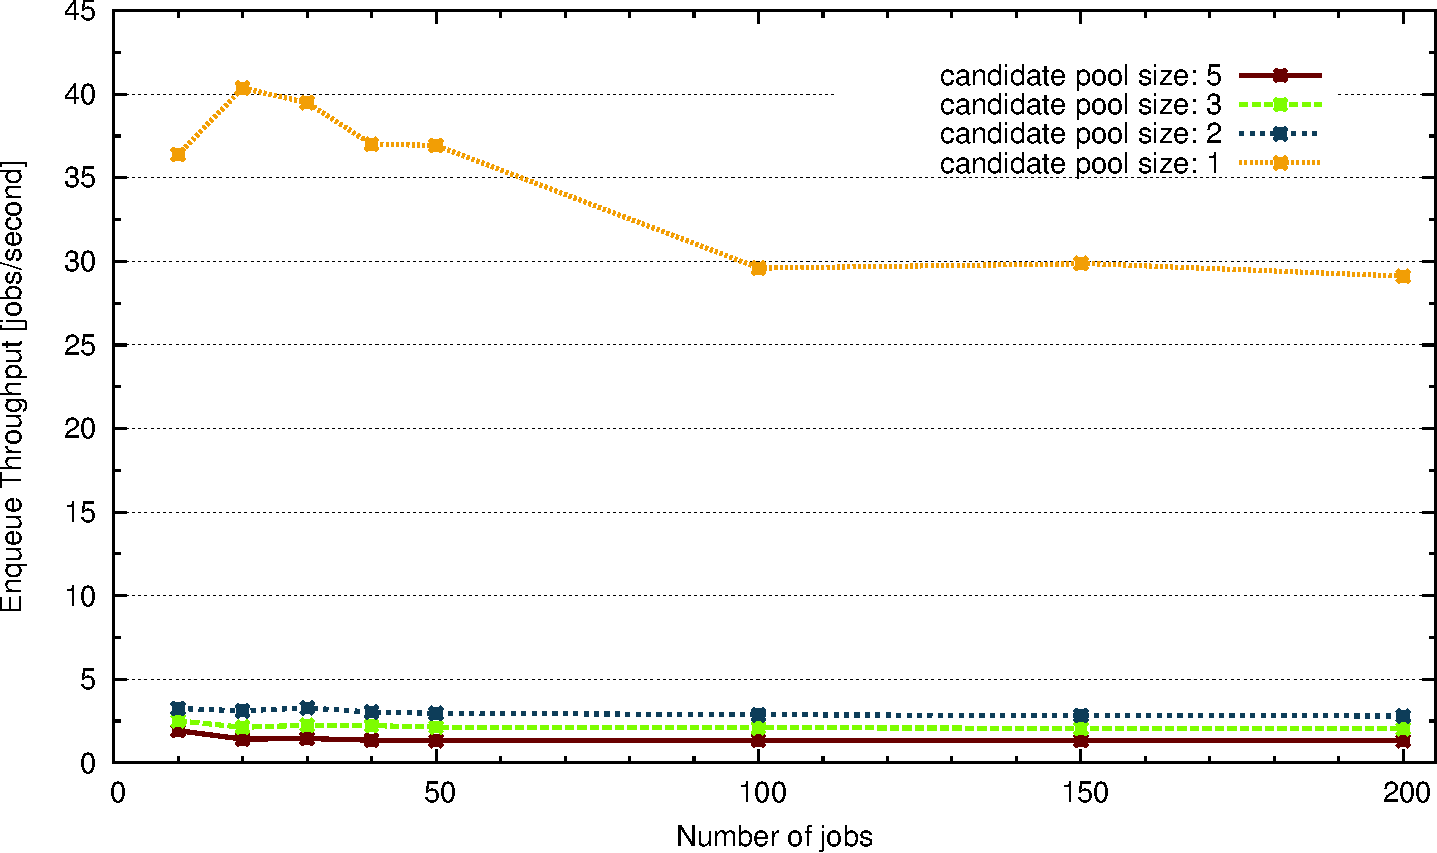
\includegraphics[width=1.0\maxwidth]{../figures/mc_comp.pdf}
    \caption{Job submission rate per number of candidates}
    \label{fig:mc_comp}
  \end{center}
\end{figure}

\begin{figure}[htbp]
  \begin{center}
    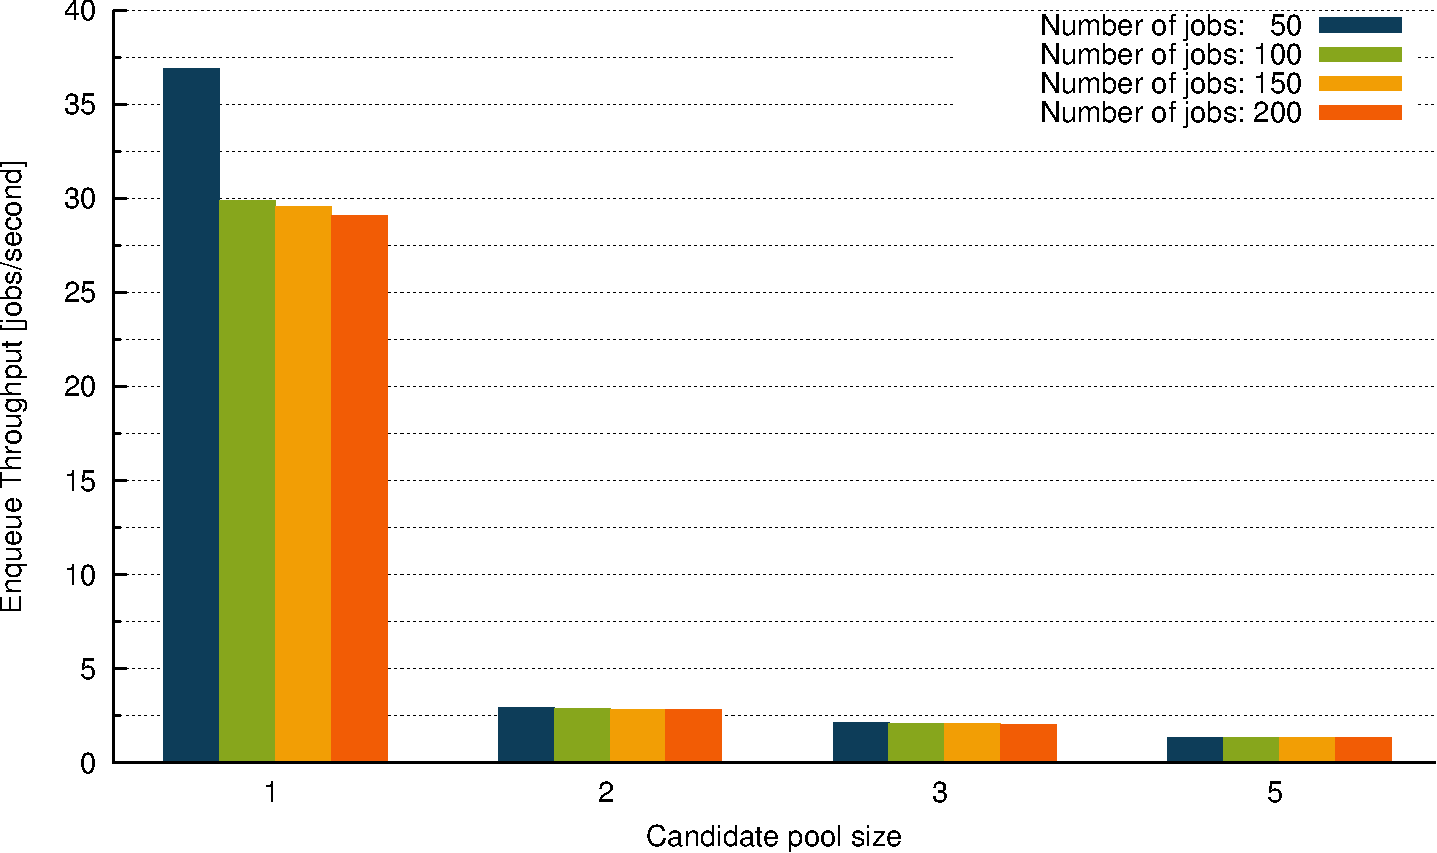
\includegraphics[width=1.0\maxwidth]{../figures/const_jobs.pdf}
    \caption{Job submission rate per number of candidates \#2}
    \label{fig:const_jobs}
  \end{center}
\end{figure}

\textbf{Performance Analysis}

There are several interesting points that we can conclude from these diagrams,
which we will address below. The most obvious observation is the significant
drop in the throughput performance, as we increase the master candidate
nodes of the cluster. Furthermore, in case of no master candidate nodes, the
distribution appears skewed characteristics and visible differentiations in the
throughput performance, something that is not observed when the candidate pool
size is increased. A closer explanation of those points follows.

In both figures, there is an obvious relationship between the job submission
rate and the number of master candidates that Ganeti maintains. As we stated in
the Caveats section, i.e., \ref{sec:caveats}, Ganeti writes jobs to disk and
then concurrently replicates them to the master candidates. The performance
slowdown of the replication process is displayed in these figures. With a single
master candidate node, we have a drop in the throughput of about \emph{8 times}
comparing to the case of no master candidates. An additional increase in the
candidate number, has no significant performance drop. This is an expected
behavior because Ganeti uses a multi-node RPC call to update the files in the
candidate nodes. This small dropdown is totally expected due to the checks that
Ganeti does after each RPC call, to get informed about the success, or not, of
the operation.

Another interesting finding from our results, are the ``outliers" that were
observed in the output sample data. When we ran the benchmarks in a cluster with
no master candidates, the data tended to have a more sparse behavior than in a
cluster with one, or more, candidate nodes. In order to make that variation
visible to the reader, we calculated the \emph{standard deviation} metric of our
distribution, which shows how much dispersion from the average value exists, and
we present it in Figure~\ref{fig:std} to justify our claim. The question that
may arise is: \emph{Why the deviation exists only in the case of a cluster with
no candidates}. The submission rate of Ganeti is the rate that the data are
written to disk, and replicated to the candidate nodes. Obviously, the disk and
network I/O are some of the factors that affect our results. As we know, Ganeti
writes the jobs to its queue, so when a worker thread grubs a job for execution,
it will subsequently update the job file in disk too. This causes
a lot of congestion in the job queue lock both from the master thread and the
job queue workers. The order that the workers grub jobs for execution causes
those differentiations in the throughput performance, in case of
no master candidates. On contrast, when the cluster contains master candidate
nodes, we have a totally smooth distribution with data around the mean value.
This behavior is justified by the replication process of the job files to the
candidate nodes. It is a quite time-consuming operation, that covers the
rest operations that are executed, and actually determines the result's form. At
this point, many types of measurements can be taken that will clarify those
claims and probably will expose more, but are out of the scope of this document
and this test category specifically, and we will not expand further.

\begin{figure}[htbp]
  \begin{center}
    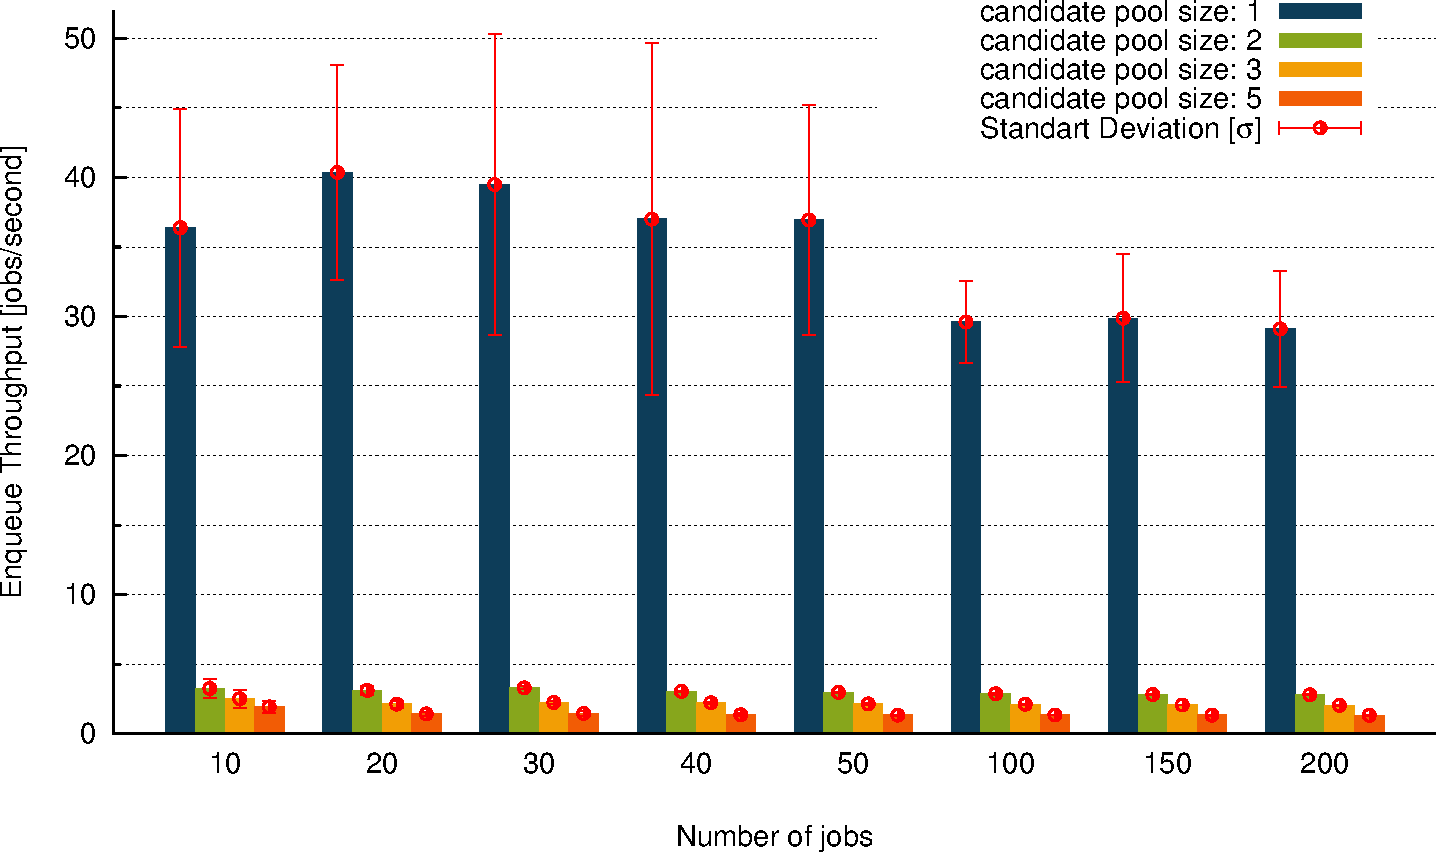
\includegraphics[width=1.0\maxwidth]{../figures/std.pdf}
    \caption{Standard Deviation [σ] of the job submission rate}
    \label{fig:std}
  \end{center}
\end{figure}

Summing up, from the results we presented, we believe that having a cluster with
two candidate nodes is the best choice to conduct the rest of our benchmarks. It
is also a choice that reflects a real production environment because it provides
the appropriate backup degree in case of a hardware failure, and also does not
have great performance impact comparing to a cluster with a single candidate
node.

\subsection{Comparison of the job submission rate}\label{subsec:enqueue_rate}

To some extend, we already discussed about the job submission performance rate
of Ganeti's default disk storage implementation, and we explained some of the
drawbacks that start to appear as the candidate pool size increases. In this
category, we make use of exactly the same metrics that we used in the previous
one, with the difference that the tests are conducted in a cluster with a
candidate pool size equal to \emph{three} nodes, as we determined in the first
benchmark category.

It is the first category where we actually compare the two driver
implementations, and we explain the main factors that affect their performance.
The results are summed up in two figures. Figure~\ref{fig:comp}, contains the
comparison of the job submission rate between CouchDB and the disk storage type,
while Figure~\ref{fig:couch_comp} presents the comparison of the CouchDB driver
performing under different socket options.

\begin{figure}[htbp]
  \begin{center}
    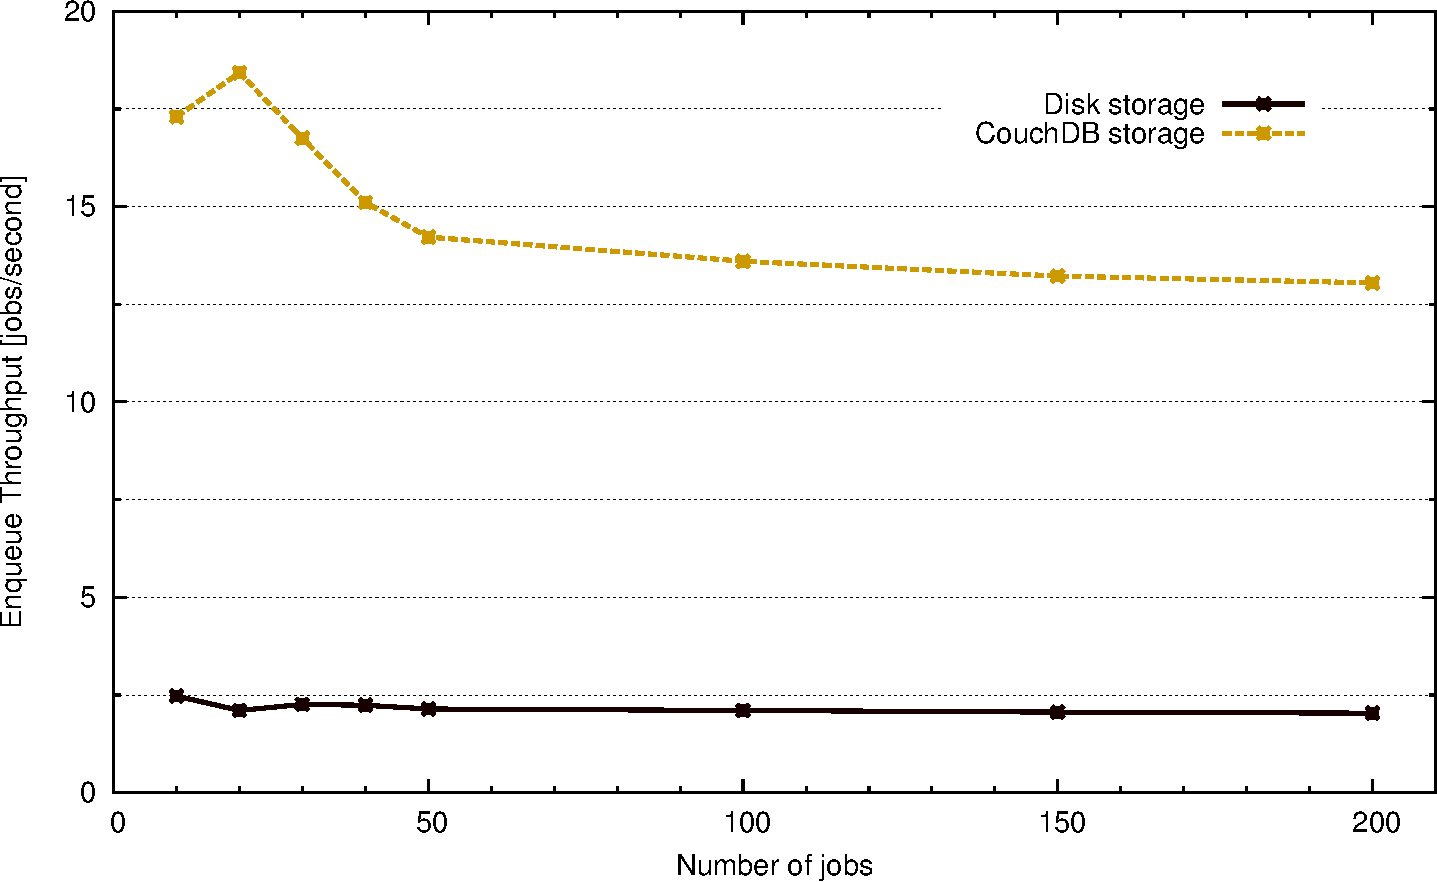
\includegraphics[width=1.0\maxwidth]{../figures/comp.pdf}
    \caption{Comparison of the throughput performance}
    \label{fig:comp}
  \end{center}
\end{figure}

\begin{figure}[htbp]
  \begin{center}
    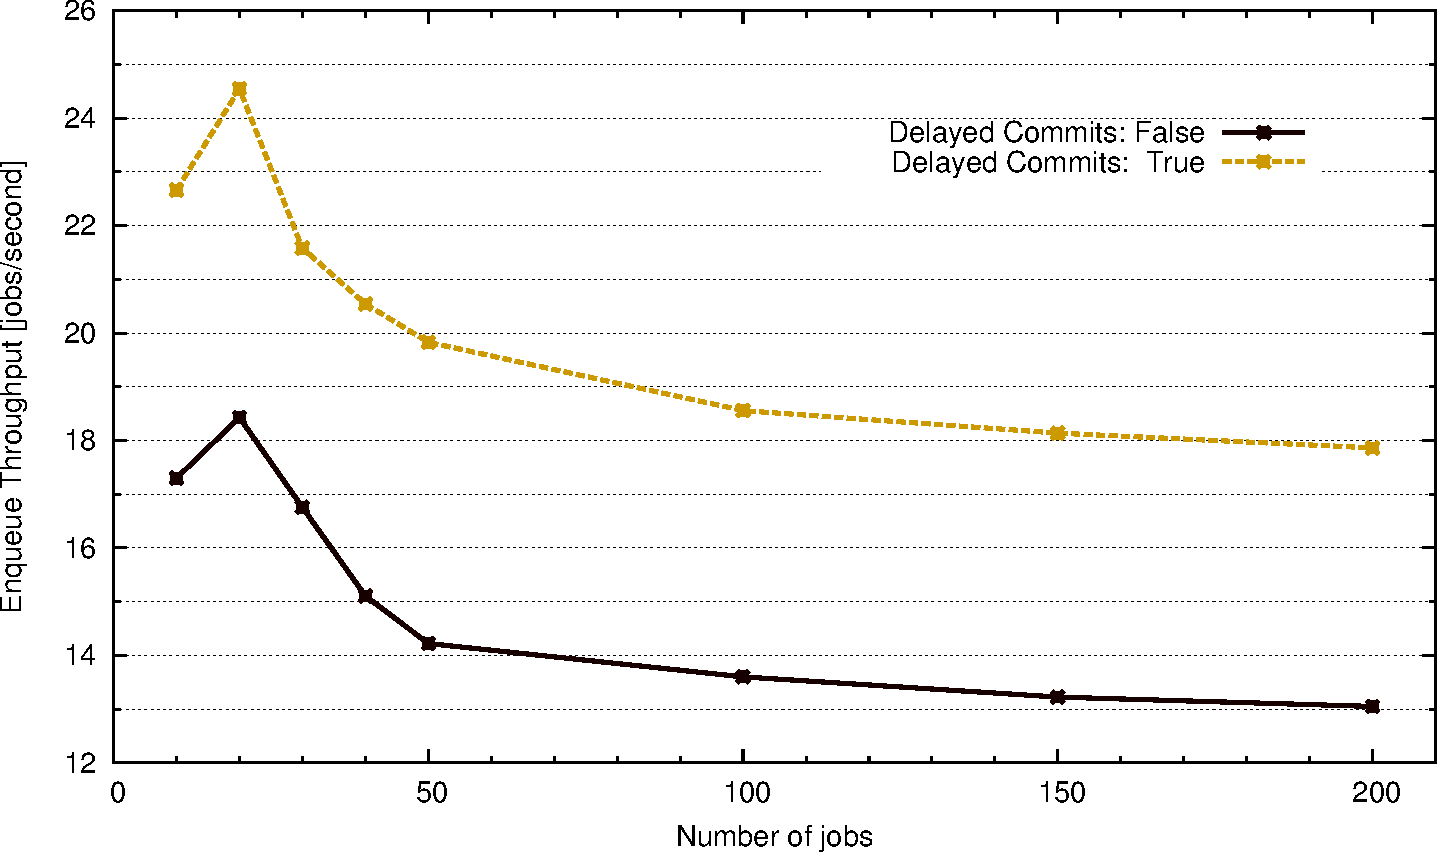
\includegraphics[width=1.0\maxwidth]{../figures/couch_comp.pdf}
    \caption{Throughput performance of CouchDB on various socket options}
    \label{fig:couch_comp}
  \end{center}
\end{figure}

\textbf{Performance Analysis}

Before we proceed with the interpretation of the diagram results, we have to
mention that the metrics we used, are exactly the same as in the first benchmark
category, and the final values correspond to the \emph{mean} value of every
distribution too.

Figure~\ref{fig:comp}, is the first performance comparison test that we
made between the two peers. The initial results look very promising. In a
\emph{5-node} cluster with two master candidate nodes, we have a speedup in the
job submission rate at about \emph{7-times} in the CouchDB driver, comparing to
the default disk storage implementation. The job submission rate has impact in
the overall job execution duration, as we will show in the last benchmark
category, and also reduces the timeouts happen in the LUXI server when many
clients try to submit jobs to Ganeti. We extensively talked about the reasons
that performance drops in a Ganeti cluster when jobs are saved to disk, in the
first test category. Now we are going to have a closer inspection in the
factors that prevent CouchDB from presenting similar behavior.

We discussed a lot about how Ganeti distributes the configuration files
to the candidate nodes, and we presented the performance impact of this
operation in the first category's figures. One of the main reasons we have
chosen CouchDB for Ganeti, is the replication feature, as it was discussed in
section~\ref{item:replication}. CouchDB is a database the replicates, and with
this term we mean that its fundamental function is to provide a simple, fast,
and convenient way to \emph{synchronize} two or more CouchDB databases.
Replication is handled completely by a separate process, external to Ganeti,
which listens on changes to the \emph{source} database, and replicates them to
the \emph{targets}. Obviously, the source refers to the master database, while
the targets are the databases of the candidate nodes. The \texttt{replicator}
process listens continually to the source's \texttt{\_changes} feed, and a new
modification to the source will immediately be replicated to the candidate
nodes. In order to ensure safety, CouchDB makes an \emph{fsync} call before a
\emph{201 Created} request is returned to the client. As soon as the
nodes are ``up" and running CouchDB will replicate, and there is no need to make
extra checks similar to the RPC checks that Ganeti has to make to find out that
the updates have reached a majority of the nodes, before declaring the
operation as successful. Instead, it is sufficient to check that the CouchDB
servers in the candidate nodes are accessible. This operation can be handled by
individual clients, independent to Ganeti that will not affect the performance,
and is an issue that is expected to be fixed in a future driver version, as we
will discuss in the Conclusion, i.e., Chapter~\ref{ch:conclusion}.

Besides the comparison test between the two implementations, we also make
a comparison test for the CouchDB drive,r on various socket options that CouchDB
provides, and have a great impact in the overall performance of the tool.
Figure~\ref{fig:couch_comp} shows this performance comparison test, on the
\texttt{delayed\_commits} attribute of CouchDB. When we set this attribute to
\texttt{True}, it is observed a further increase in the throughput performance
at about \emph{9-times} comparing to the default disk implementation, and at
about \emph{35\%} comparing to the CouchDB driver with this attribute set to
\texttt{False}. Delayed commits is probably the most important CouchDB
configuration setting for performance. When is set to true (the default),
CouchDB allows operations to be run against the disk without an explicit
\emph{fsync} call after each operation. Fsync operations take time in order to
complete, and calling them on each update limits the CouchDB performance for
sequential writers. It is clear that setting this option to true, opens a
window for data loss, because data are being kept in a write buffer and are
fsync-ed after a certain amount of time, or when the buffer is full. Ganeti is
an environment where we absolutely need to know when the updates have been
received, so we set this attribute to false, by default. The aim of this
test, is to expose an important setting of CouchDB that could be enabled
periodically, in several cases, like in a situation with an overloaded master
daemon, and then disabled at will. It is up to the cluster administrator to
measure the tradeoff between loosing some data in case of a hardware failure,
and the ``relief" that the performance improvement will bring to the cluster.

To achieve the results we presented for the CouchDB driver, another
important configuration option must be modified, related to the TCP buffering
behavior. This is the \emph{nodelay} option which must be set to \texttt{True},
in order to disable the \emph{Nagle's algorithm}~\flink{http://en.wikipedia.org/
wiki/Nagle\%27s\_algorithm}, which introduces an additional delay when using
keep-alive HTTP-connections. By setting this option to true, the
\emph{TCP\_NODELAY} option is turned on for socket, which means that even small
amounts of data sent to the TCP socket, like the reply to a document write
request, or reading a very small document, will be sent immediately to the
network. They will not be buffered hoping that it will be asked to send more
data through the same socket in order to transfer them all at once. The main
reason that this important option is disabled by default, is that the last
releases of CouchDB ships with a more recent version of the HTTP server library
\emph{MochiWeb}~\flink{https://github.com/mochi/mochiweb}, which by default sets
the \emph{TCP\_NODELAY} socket option to false.

\subsection{Comparison of the config.data performance}\label{subsec:config_perf}

The CouchDB driver, besides the alternative storage solution that provides to
the configuration files of Ganeti, also introduces a variation in the
way it handles the \texttt{config.data} file, as it was extensively discussed
in Section~\ref{sec:config}. The ultimate aim of this category is to compare the
performance of the two alternative implementations of handling the configuration
file, but before we reach to this point, we will investigate in deep all the
factors that affect the configuration file performance, and that were discussed
in Section~\ref{sec:caveats}.

In this category we will present three diagrams in total. The first two
of them [\ref{fig:total-cfg}, \ref{fig:couchdb}], one for each driver,
show the total execution duration of the \texttt{\_WriteConfig} method, and all
the sub-method calls that are been made. This is the responsible method for
applying the changes of the configuration file to the permanent storage, and
replicate them to the master candidate nodes.
Every operation that modifies the cluster state calls this function to
make the changes permanent. It is the most time consuming function related to
the configuration file, and has a great importance in the performance of Ganeti,
because is must be called with the \texttt{ConfigWriter} lock held in exclusive
mode, which starts to become a bottleneck when a huge number of jobs is in
execution. If we manage to reduce the time the lock is held by the workers, we
will also reduce some of the congestion in the config lock. The last diagram
[\ref{fig:comp-cfg}], is the actual performance comparison plot between the two
implementations.

The benchmarks of this section have been conducted on a cluster with a candidate
pool size equal to \texttt{one}, \texttt{three}, and \texttt{five} nodes,
respectively. In order to measure the performance of the \texttt{\_WriteConfig}
method, we intentionally increased the size of the \texttt{config.data} file,
from \texttt{100 KB} up to \texttt{5 MB}. A cluster with about \emph{2.000}
instances has a configuration file of around \texttt{5 MB}, which corresponds to
a real workload for a production environment. Our test concentrates on modifying
a parameter of a single configuration object. We chose an instance object as a
use case. Starting, restarting, or stopping an instance is a quite commonly used
operation, that while it aims to modify a single field of the instance object,
the whole configuration object is flushed to disk, and moreover the
\texttt{ssconf\_*} files are not affected; a variance that we do not want
to take into account in this test category. The test was repeated \emph{20}
times for each pair, and we find it appropriate to make use of the
\emph{trimmed mean} value of our distribution. The trimmed mean is a method of
averaging, that removes a small percentage of the largest and the smallest
values before calculating the mean. This method aims to reduce the effects of
the outliers on the calculated average, and stated as mean trimmed by
\emph{X\%}, where \emph{X} is the sum of the percentage of observations
removed from both the upper and lower bounds. In our case, we trimmed the mean
by \emph{20\%}. The reason we did not calculate the normal mean value, is that
we wanted to reduce the effects of the outliers that were observed, and to
obtain a more accurate average performance overview, for both the
implementations.

\bigskip
\textbf{Performance Analysis}

In the begging of our analysis, we will take a closer inspection on all the
factors related to the performance of the write operation of the
configuration file. An operation that affects the configuration state, passes
from the following execution phases in general. Firstly, some preliminary checks
are being made on the object that it is requested to change, and then the
update of the in-memory representation of the \texttt{config.data} object
follows. Then the \texttt{\_WriteConfig} method is called, which flushes the
updates to disk, and replicates them to the candidate nodes. This method
consists of a number
of time-consuming sub-method calls that affect the overall performance of any
cluster operation that modifies the configuration file. These calls contain the
verification of the config object for configuration errors, to maintain the
consistency of the object, and is named \texttt{\_UnlockedVerifyConfig}, the
serialization of the config object in order to be prepared for applying the
changes to disk, through the \texttt{serializer.Dump} call, and then the actual
flushing of the in-memory object to disk, using the \texttt{utils.SafeWriteFile}
function call. Finally, the modifications have to be replicated to the candidate
nodes with the \texttt{\_DistributeConfig} method. All these operations are
affected from the size of the configuration file, and from the candidate pool
size as well. Figure~\ref{fig:total-cfg}, extensively examines this behavior.

From Figure~\ref{fig:total-cfg}, the following conclusions can be made. The most
time-consuming method, is the serialization of the configuration file. It
is a totally independent cost from the candidate pool size, but it is 100\%
bounded with the size of the file. The file is stored in
memory as a \texttt{ConfigData} object, a generic config object defined by
Ganeti. In order to be saved to disk, it must be transformed to a string format,
and this is the role of this method. The cost of the file replication to the
candidate nodes is increases along with the number of master candidates, and the
size of the file too. In the same sense, the verification check consumes a lot
of time in bigger file sizes because it traverses the whole file, same as the
time of the function that applies the changes to disk, but with the difference
that even in bigger file sizes it
does not consume a noticeable amount of time. From this diagram it is understood
that in a cluster with three candidate nodes, even from a file of \emph{1.0 MB}
in size, it takes at about \emph{1 sec} to complete a single operation.
If we combine it with the congestion on the config lock, we can see
the great impact of that delay in the overall cluster's performance.

It is obvious that a single configuration file comes with a number of
disadvantages. Modifying a single field of the file requires the serialization
of the whole config object and the distribution to the candidates, as well. This
approach reduces the cluster performance due to the increased operational cost
that is implied. In Figure~\ref{fig:couchdb}, we will present a different
approach that the CouchDB driver introduces, by conducting the same test on the
\texttt{\_WriteConfig} method of the CouchDB driver.

In Figure~\ref{fig:couchdb}, we observe a great improvement in the total
execution duration of updating the configuration file. This differentiation can
be justified by the different approach of CouchDB of handling the config object.
The configuration file has been separated to its sub-components, as
we extensively discussed in section~\ref{item:config}. Modifying an instance, a
node, and generally a single object of the configuration file, does not updates
the whole object to disk, but only the single object we want to.
Moreover, the serialization cost does not
implies anymore. The transformation of an object before it is written to disk
is a simple conversion to dictionary, and it is part of the
\texttt{utils.WriteDocument} method. Since we convert only few kilobytes each
time the cost is negligible. The distribution cost is also disappears due to
the different approach of CouchDB on handling the replication process, as we
already extensively explained. The verification cost is the only one that does
not changes, since we continue to verify the whole in-memory configuration
object.

The last diagram we are going to present in this category, is presented in
Figure~\ref{fig:comp-cfg}. It displays the total execution duration of an
instance modify operation. It is a representative job, as all Ganeti operations
modify a specific field of the configuration file. The same output would appear
if we were modifying a node, a network, or a nodegroup. As we said in the
\emph{Implementation Details} section of the CouchDB driver, i.e., Section
\ref{sec:couch_details}, every update causes two consecutive object updates to
the CouchDB server. One for the cluster general information, and one for the
object we want to change. In this figure, we present the total execution time
for CouchDB, that is the aggregated execution duration of the two objects.
Even with this overhead the difference of flushing the whole file to disk
comparing to the single object that is updated is significant. For example, for
a file of \emph{2 MB} in size, we have at about \emph{5-times} increase in the
performance of CouchDB, while the gap is widening as the file size further
increases.

\begin{figure}[htbp]
  \begin{center}
    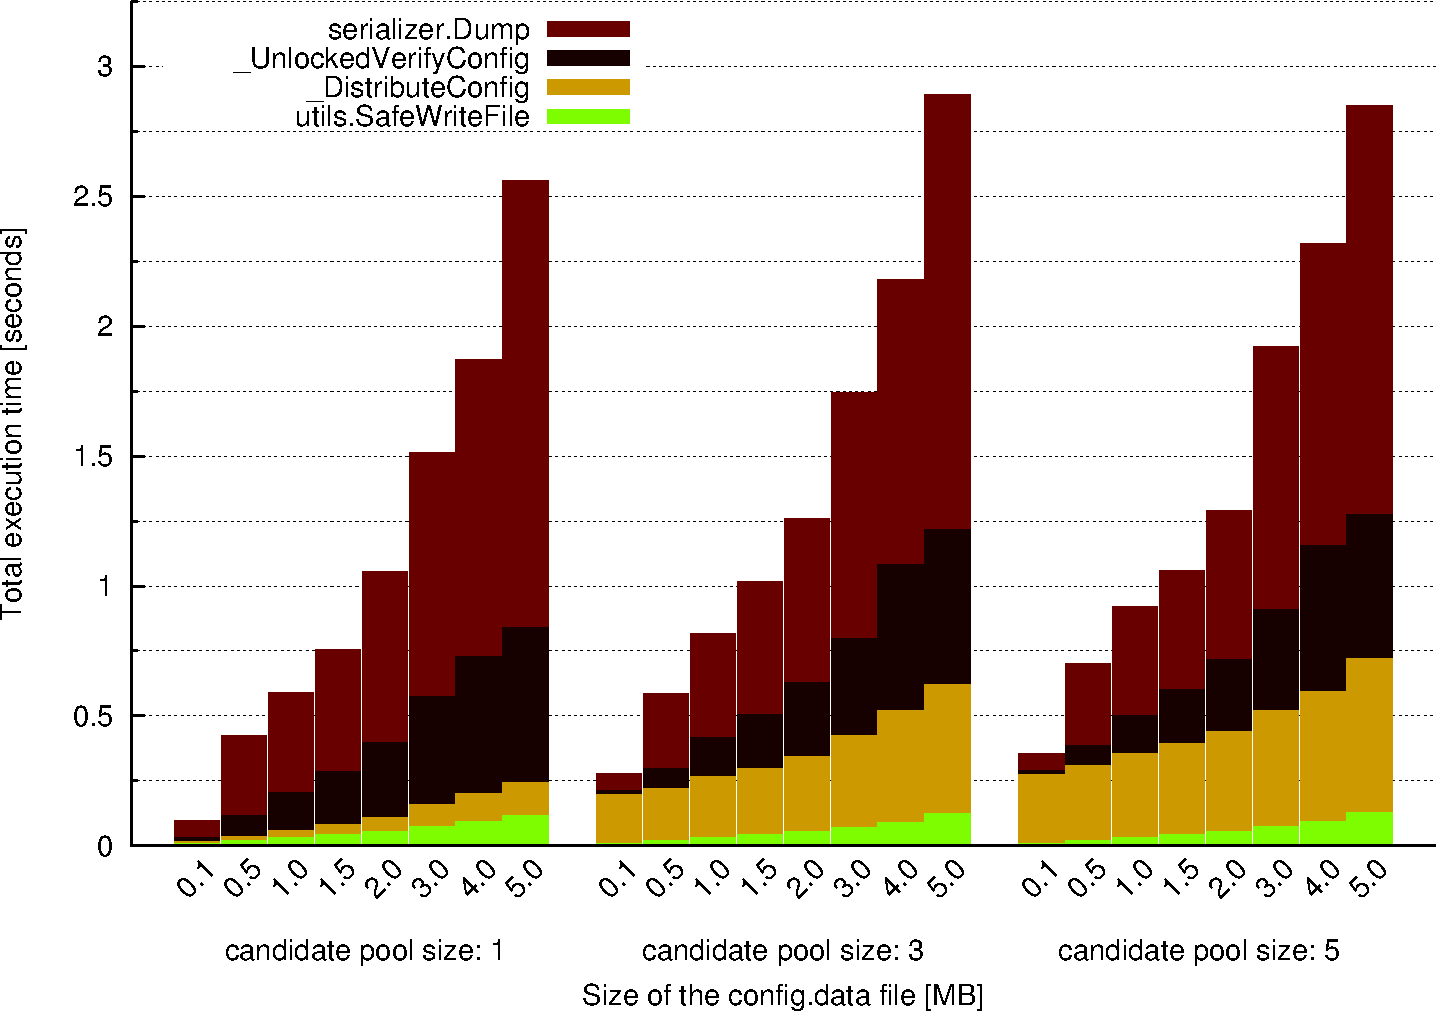
\includegraphics[width=1.0\maxwidth]{../figures/total-cfg.pdf}
    \caption{Performance evaluation of the default \_WriteConfig method}
    \label{fig:total-cfg}
  \end{center}
\end{figure}

\begin{figure}[htbp]
  \begin{center}
    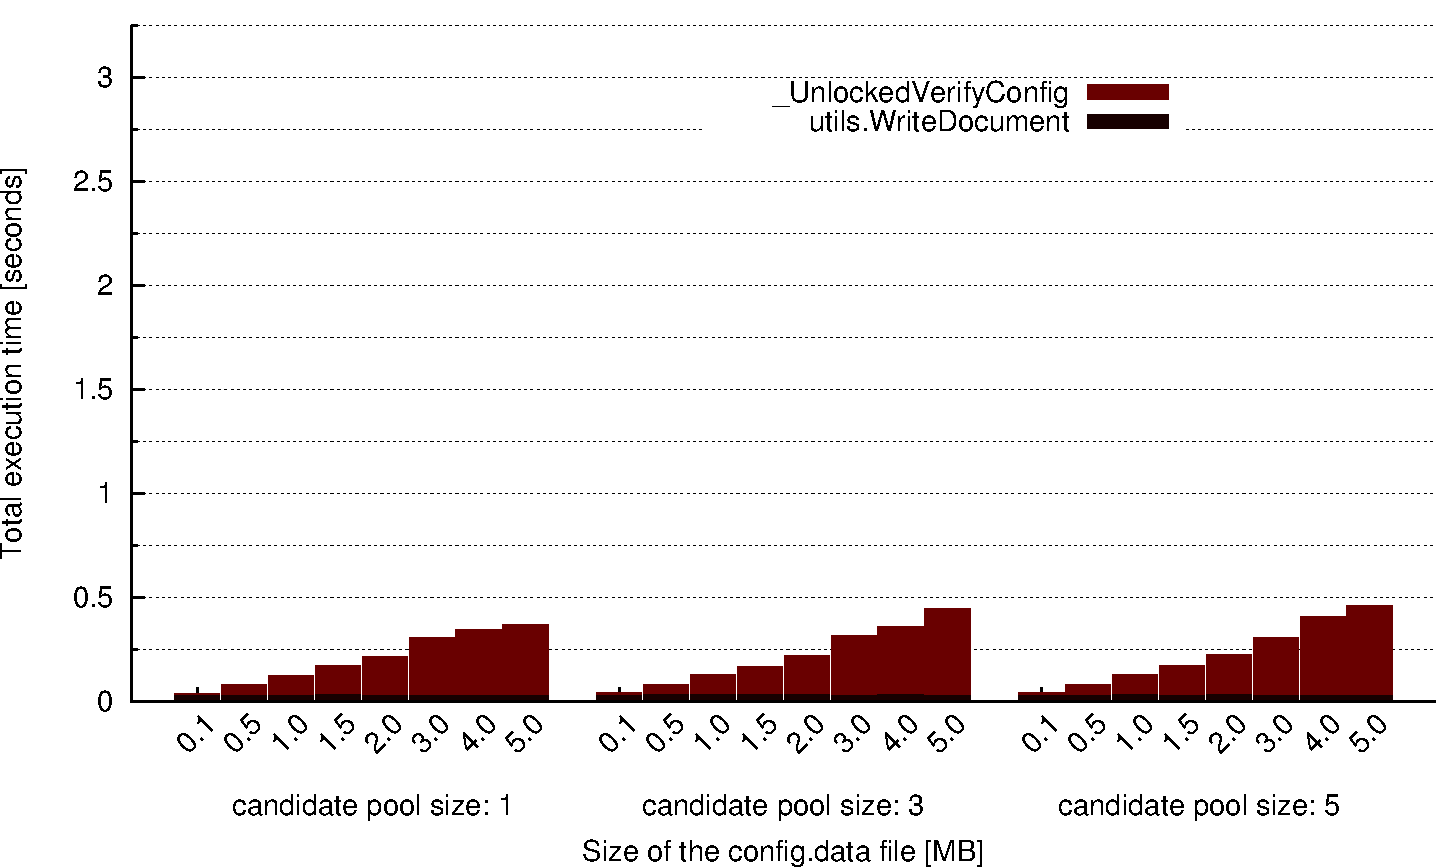
\includegraphics[width=1.0\maxwidth]{../figures/couchdb.pdf}
    \caption{Performance evaluation of the \_WriteConfig method of CouchDB}
    \label{fig:couchdb}
  \end{center}
\end{figure}

\begin{figure}[htbp]
  \begin{center}
    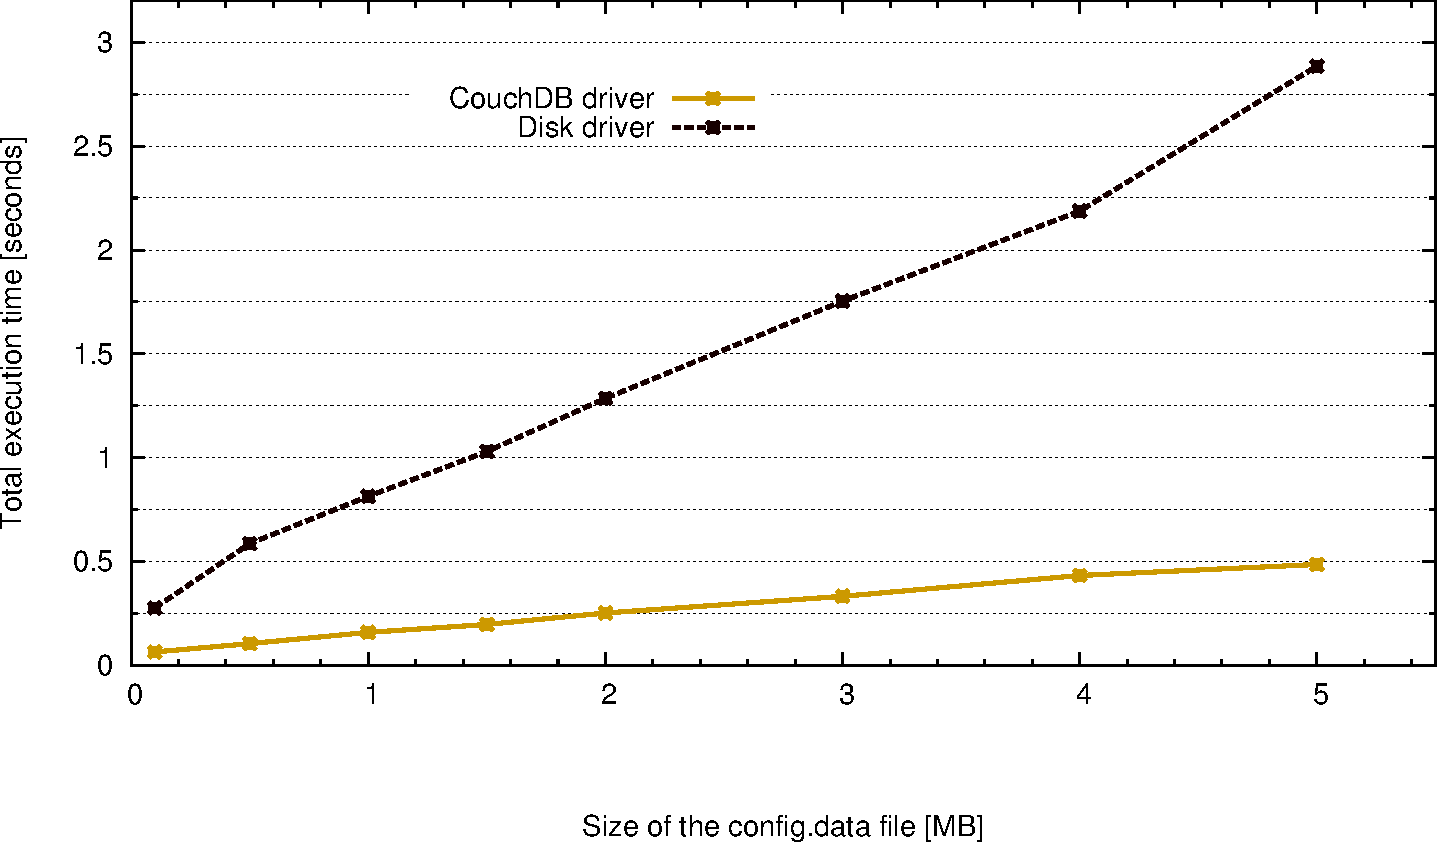
\includegraphics[width=1.0\maxwidth]{../figures/comp-cfg.pdf}
    \caption{Comparison of execution performance for instance modify ops}
    \label{fig:comp-cfg}
  \end{center}
\end{figure}

\subsection{Aggregate evaluation of the CouchDB driver}\label{subsec:total_eval}

Up to this point, we have tested our implementation in a variety of situations
that may occur in a Ganeti cluster. We also examined some of the main factors
that limit Ganeti from scaling and achieving better performance. In this last
benchmark category, we will attempt to measure the overall performance of
our drivers in a real-world scenario. In order to explain the results of this
section, we will also make use of the findings from the previous categories.

In a Ganeti cluster with \emph{5 vm-capable} nodes, and three master candidates,
we will concurrently submit jobs of \emph{OpInstanceCreate} opcodes, in batches
of \texttt{1}, \texttt{10}, \texttt{20}, \texttt{50}, and \texttt{100} jobs. We
will measure the average time of the phases that a job passes through, and then
the total execution duration from the first job that it is enqueued since the
last that is completed. Since the \texttt{Running} times of the jobs are
independent to the underlying storage layer that it is used, we will minimize
it by creating instances with \emph{1 GB} file disk, using the
\emph{--no-install}, \emph{--no-start} options that disable the OS installation
and the start-up of the instances respectively.

\bigskip
\newpage
\textbf{Performance Analysis}

Figure~\ref{fig:jobs_avg}, displays the average duration of the execution phases
of the \emph{InstanceCreate} jobs we submitted. For a short reminder about the
execution phases of a job, refer to Section~\ref{subsec:jobs}.

\begin{figure}[htbp]
  \begin{center}
    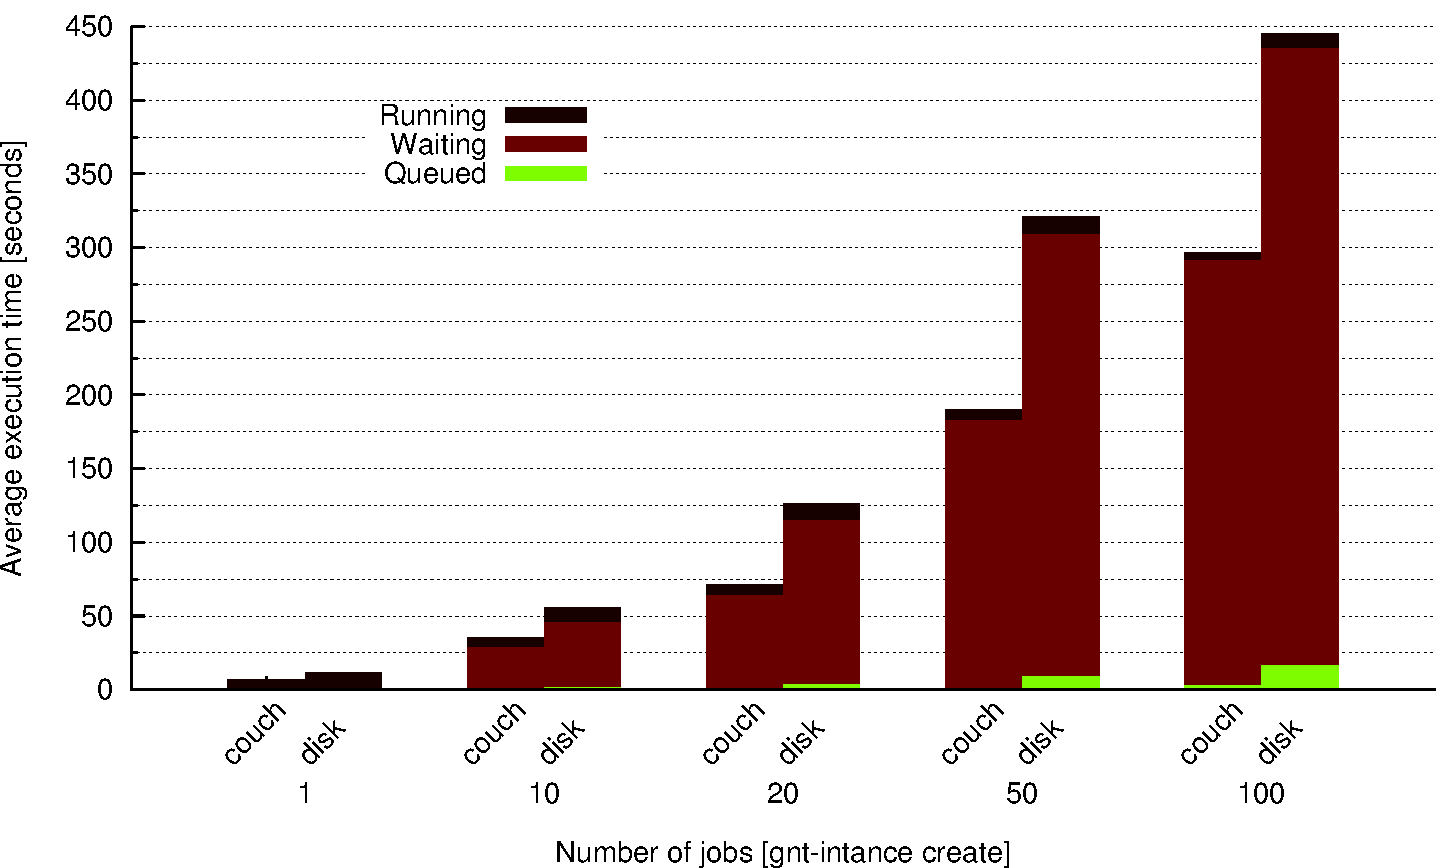
\includegraphics[width=1.0\maxwidth]{../figures/jobs_avg.pdf}
    \caption{Comparison of execution performance for the phases of a job}
    \label{fig:jobs_avg}
  \end{center}
\end{figure}

What we observe from Figure~\ref{fig:jobs_avg}, is a minimized \emph{Running}
time for reasons we already covered, while the most time is consumed in the
\emph{Waiting} phase. In this phase the jobs are waiting for locks, held by other
threads that are in execution. The \emph{Opportunistic locking} that it is used
since Ganeti version \emph{2.7}, improved the lock congestion in instance create
operations, but since we create a lot of instances in a small cluster, it is a
normal behavior. It is also observed that the average time of CouchDB in the
\emph{Queued}, and \emph{Waiting} phase is quite smaller comparing to the disk
implementation. We already covered the improved performance in the submission
rate of CouchDB. The new finding, is the increase in the average \emph{Waiting}
performance time. This behavior can be justified by the increased job submission
rate, as we presented in Figure~\ref{fig:comp}. The worker threads, are waiting
in the queue for new jobs to appear. As soon as a job is submitted in the queue,
and a worker thread is available, it grubs it for execution. An increased job
enqueue rate translates to workers that acquire their workload earlier. As a
result, we have an immediate impact in the \emph{Waiting} average time, due to
the fact that the workers are idle for less time than they previously were, and
the resources of the cluster are exploited more efficient than before. An
immediate consequence of the increase in the performance of the \emph{Queued}
and \emph{Waiting} time, is an increase in the total execution duration of the
jobs. This induction is justified by~Figure~\ref{fig:total_secs}.

\begin{figure}[htbp]
  \begin{center}
    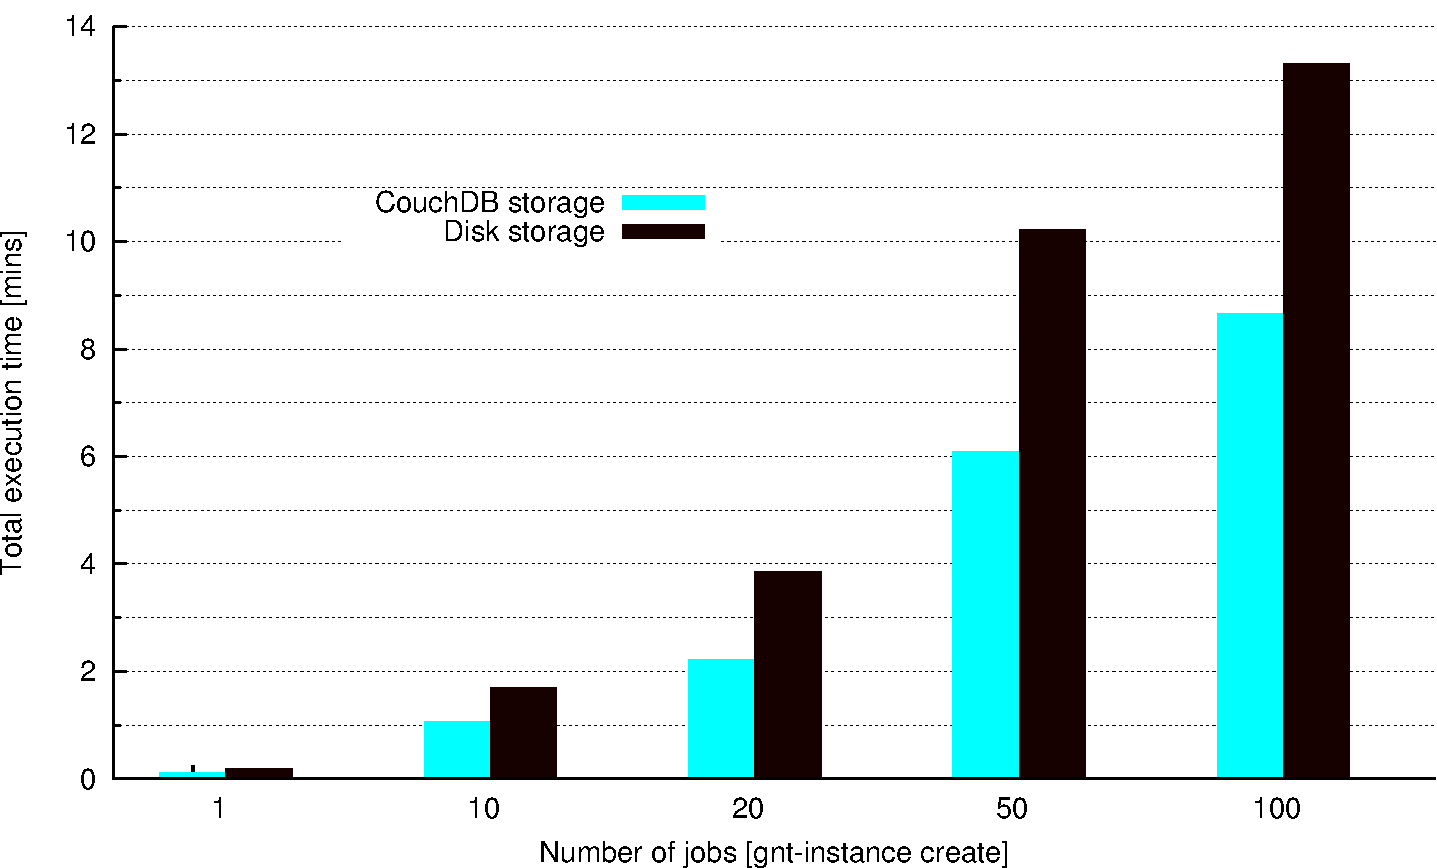
\includegraphics[width=1.0\maxwidth]{../figures/total_secs.pdf}
    \caption{Comparison of the throughput performance for instance create ops}
    \label{fig:total_secs}
  \end{center}
\end{figure}

What we conclude from Figure~\ref{fig:total_secs}, is that the CouchDB driver
performs better under a heavy loaded environment. The performance gap between
the two implementations widens as the number of jobs in the cluster increases.
CouchDB is designed to service highly concurrent use cases, and perform under a
heavy application load. The \emph{Multi-Version Concurrency Control} that
implements, makes CouchDB able to handle a high volume of concurrent readers and
writers without conflicts to each other. As a result, there will not appear any
performance gaps as the cluster workload is increased, and the requests will
continue to be serviced efficiently.

\chapter{Conclusion}\label{ch:conclusion}

\section{Concluding remarks}\label{sec:remarks}

This thesis described the design decisions, the technical-issues, and the
implementation details for replacing the Ganeti configuration and job queue
storage engine with CouchDB, a distributed document-oriented database. The goal
of this thesis was to examine if it was \emph{feasible} to integrate a NoSQL
database system in Ganeti, and measure the \emph{efficiency} of this approach.

After introducing the necessary theoretical background information about
Ganeti and all the related fields of interest, we presented the main drawbacks
that Ganeti appears, and the options that were evaluated to chose a NoSQL
system, and specifically CouchDB, to provide a solution to some of those issues.
We continued with the design and implementation details of the new storage
choice, and finally we evaluated our solution, in regard to two broad
dimensions: performance, and scalability potentials. Special attention was given
on being fully compliant with the current Ganeti requirements, such as
maintaining the fault-tolerant attribute by putting the safety of the data
first, security, and mainly not intervening with the parts of the Ganeti code
that are not related with our implementation.

Looking back at what we have created, we can say that we also covered another
need of Ganeti. The modular approach we followed for our design, supports both
CouchDB and file configuration as different storage engines, with different
limitations for each case. The current storage options can be easily extended
due to the transformation that we made to the base configuration modules, and we
could provide support for additional engines, such as MongoDB, or any other
option that would fit the requirements of Ganeti. As far as the implementation
complexity of the abstraction of some modules is concerned, we agree that we
introduced an important amount of transformations to the code, but taking into
account the extra features it introduces, and the fact that the code base is
quite clear and straightforward, we can state that the benefits are greater than
the cons, and the implementation can be consider \emph{successful}.

Benchmark results were quite promising. Both the storage engines have been
tested under various use cases and workloads. We measure the performance using
a variety of metrics which we believe that correspond to a real-world
environment. We have also studied the reasons that we consider responsible for
the differentiations that appeared in the performance of the two engines. Based
on this examination, we conclude that there are good indications that the NoSQL
approach will be able to give extra choices and provide additional support, to
the single storage solution which is currently used by Ganeti.

We admit that there are more factors we should consider before trying this new
approach to a real production environment. Since we are only in the first
version of the CouchDB driver, and since some of the limitations we presented
are fixed as of writing this chapter, and also considering the important
performance gains we observed, we strongly believe that this work can become the
basis for further work, and give the motivation for focusing on different
approaches for the Ganeti storage engine. A further integration of this design
in a demo environment, will help us gain the desirable feedback for more
improvements, and perhaps will provide us the basis for new ideas and feature
extensions.

\section{Future work}\label{sec:future}

The development of our implementation is far from over, as the tool has a lot of
room for further improvements. Our tasks for the future, on some of which we are
currently working on, will be classified into two separate categories. The
short-term goals, and the long-term ones, which are the following:

\subsection{Short-term plans}

This section, mainly contains improvements of the current implementation, and
the extension of the existing functionality.

\begin{description}
  \item[Fixing configuration ACID issue] \hfill \\
    In Section~\ref{sec:couch_details}, we discussed an issue that arisen from
    the transformation of the \texttt{config.data} file management. It is
    our primary priority dealing with this irregularity, and provide an
    efficient solution that will fix that issue, without affecting the overall
    performance of the tool.
  \item[Verification of the replication process] \hfill \\
    Currently, we do not make any kind of verification checks on the replication
    process. We do not have a way to ensure if a modification reached a majority
    of the candidate nodes, but we are based on the CouchDB server integrity.
    CouchDB will replicate, and all files will reach their destinations, as
    long as the server is running. We would like an external to Ganeti process,
    verify the status of the CouchDB instances, and warn the user for a possible
    failure. The current \texttt{ganeti-watcher} script, is a possible candidate
    that can be extended to provide the desired functionality, but more
    solutions can be discussed.
  \item[Improving the ssconf\_* management] \hfill \\
    Ganeti maintains the \texttt{ssconf\_*} set of files in all the nodes of the
    cluster. As a result, in an operation that modifies one or more of those
    files, the cost of applying the changes among the nodes of the cluster is
    aggregated. This cost is not negligible, and is one of the reasons that
    forbids Ganeti from scale. We could also add those files to the CouchDB
    server in a separate database called \texttt{ssconf}, and share this
    information only among the candidate nodes. Since, every node needs to have
    access to those files, we could give write permissions to the master node,
    while the rest nodes will only have read permissions to the database. It is
    an important performance fix which is intended to be applied soon.
  \item[Import all cluster information] \hfill \\
    Currently, CouchDB hosts only the job queue, the archive directory, and the
    \texttt{config.data} file. The rest Ganeti information, such as the SSL
    certificates, the daemon related keys, or the abovementioned
    \texttt{ssconf\_*} set of files, continues to be stored in the filesystem.
    We would like to import all those information in the CouchDB server, as
    well.
  \item[Backups for disaster-recovery] \hfill \\
    Ganeti keeps a backup for the configuration data file, as soon as a node is
    demoted from the master candidate role. CouchDB does not follow with this
    requirement. The code will be converted to follow that requirement, and
    subsequently it may be extended to keep flat backup files periodically, to
    add an extra layer of protection from hardware failures.
\end{description}

\subsection{Long-term plans}

This section contains our thoughts about extending Ganeti, improving its
overall performance, and its ability to scale better in bigger clusters.

\begin{description}
  \item[Improving candidate pool management] \hfill \\
    At this point, the CouchDB driver does not affect the management of the
    candidate nodes. Each node in the cluster has a running CouchDB server. As
    soon as a node is marked as candidate, the master node will extend its
    replication tasks to include this node as well. We are currently discussing
    another approach of managing the pool of candidate nodes. We could keep a
    set of hosts, even independent to Ganeti, that will be used for the
    candidate pool requirements only. These hosts will contain the live cluster
    configuration and the job queue information, which they will be shared. The
    master node will interact with those databases to store the cluster
    information, removing the requirement of maintaining the candidate pool
    exclusively inside Ganeti nodes. Using \emph{Solid State Drives (SSDs)}
    in that small set of nodes is more feasible than in a whole cluster, and it
    will be really handy for CouchDB.
  \item[Clustering support] \hfill \\
    The above idea can be amplified by the clustering techniques that the NoSQL
    systems provide. Since the NoSQL systems are designed to serve large data
    sets, some additional features are introduced to provide redundancy and
    high-availability in any case. Clustering and auto-sharding are some of
    those features, that provide the ability to the NoSQL systems to store and
    share data across multiple machines, using efficient algorithms for handling
    the read/write requests, and support the data growth demands. Currently,
    CouchDB supports clustering using external applications such as
    \emph{CouchDB Lounge}~\flink{http://tilgovi.github.io/couchdb-lounge/}. The
    merge of CouchDB that was announced with BigCouch, a Cloudant's clustered
    version of CouchDB, will bring soon all the clustering capabilities that
    currently CouchDB lacks of. Besides the facilitation in handling the set
    of candidate nodes, since they will be part of the cluster, with BigCouch
    merged in, CouchDB and Ganeti consequently will be able to replicate data at
    a much larger scale.
  \item[Extending storage choices] \hfill \\
    Abstracting the related to the storage management code of Ganeti, was our
    number one priority. We made it feasible to easily create additional storage
    engines for Ganeti. Moreover, the similarity among the NoSQL family that
    exists, can be exploited to design new driver solutions, such as
    \texttt{MongoDB}~\flink{http://www.mongodb.org/}, compare their performance,
    and generally having the ability to choose among several storage options
    according to our application's needs.
  \item[Improving lock congestion] \hfill \\
    The NoSQL systems are using their own locking policy. CouchDB uses the
    \texttt{MVCC} method to handle read and write requests. MongoDB
    uses a \texttt{readers-writer}, or \texttt{shared exclusive} per
    database lock, to deal with concurrent readers and writers. We could improve
    the current locking situation and be based on the locking level layer
    providing by the NoSQL systems. The \texttt{ConfigWriter}, and the queue
    level lock are the first contenders to be removed, since any serialization
    to accessing the configuration file and the job queue would be unnecessary.
\end{description}

\chapter{Προτάσεις για μελλοντική έρευνα}\label{ch:conclusion}

\section{Concluding remarks}\label{sec:remarks}

This thesis described the design decisions, the technical-issues, and the
implementation details for replacing the Ganeti configuration and job queue
storage engine with CouchDB, a distributed document-oriented database. The goal
of this thesis was to examine if it was \emph{feasible} to integrate a NoSQL
database system in Ganeti, and measure the \emph{efficiency} of this approach.

After introducing the necessary theoretical background information about
Ganeti and all the related fields of interest, we presented the main drawbacks
that Ganeti appears, and the options that were evaluated to chose a NoSQL
system, and specifically CouchDB, to provide a solution to some of those issues.
We continued with the design and implementation details of the new storage
choice, and finally we evaluated our solution, in regard to two broad
dimensions: performance, and scalability potentials. Special attention was given
on being fully compliant with the current Ganeti requirements, such as
maintaining the fault-tolerant attribute by putting the safety of the data
first, security, and mainly not intervening with the parts of the Ganeti code
that are not related with our implementation.

Looking back at what we have created, we can say that we also covered another
need of Ganeti. The modular approach we followed for our design, supports both
CouchDB and file configuration as different storage engines, with different
limitations for each case. The current storage options can be easily extended
due to the transformation that we made to the base configuration modules, and we
could provide support for additional engines, such as MongoDB, or any other
option that would fit the requirements of Ganeti. As far as the implementation
complexity of the abstraction of some modules is concerned, we agree that we
introduced an important amount of transformations to the code, but taking into
account the extra features it introduces, and the fact that the code base is
quite clear and straightforward, we can state that the benefits are greater than
the cons, and the implementation can be consider \emph{successful}.

Benchmark results were quite promising. Both the storage engines have been
tested under various use cases and workloads. We measure the performance using
a variety of metrics which we believe that correspond to a real-world
environment. We have also studied the reasons that we consider responsible for
the differentiations that appeared in the performance of the two engines. Based
on this examination, we conclude that there are good indications that the NoSQL
approach will be able to give extra choices and provide additional support, to
the single storage solution which is currently used by Ganeti.

We admit that there are more factors we should consider before trying this new
approach to a real production environment. Since we are only in the first
version of the CouchDB driver, and since some of the limitations we presented
are fixed as of writing this chapter, and also considering the important
performance gains we observed, we strongly believe that this work can become the
basis for further work, and give the motivation for focusing on different
approaches for the Ganeti storage engine. A further integration of this design
in a demo environment, will help us gain the desirable feedback for more
improvements, and perhaps will provide us the basis for new ideas and feature
extensions.

\section{Future work}\label{sec:future}

The development of our implementation is far from over, as the tool has a lot of
room for further improvements. Our tasks for the future, on some of which we are
currently working on, will be classified into two separate categories. The
short-term goals, and the long-term ones, which are the following:

\subsection{Short-term plans}

This section, mainly contains improvements of the current implementation, and
the extension of the existing functionality.

\begin{description}
  \item[Fixing configuration ACID issue] \hfill \\
    In Section~\ref{sec:couch_details}, we discussed an issue that arisen from
    the transformation of the \texttt{config.data} file management. It is
    our primary priority dealing with this irregularity, and provide an
    efficient solution that will fix that issue, without affecting the overall
    performance of the tool.
  \item[Verification of the replication process] \hfill \\
    Currently, we do not make any kind of verification checks on the replication
    process. We do not have a way to ensure if a modification reached a majority
    of the candidate nodes, but we are based on the CouchDB server integrity.
    CouchDB will replicate, and all files will reach their destinations, as
    long as the server is running. We would like an external to Ganeti process,
    verify the status of the CouchDB instances, and warn the user for a possible
    failure. The current \texttt{ganeti-watcher} script, is a possible candidate
    that can be extended to provide the desired functionality, but more
    solutions can be discussed.
  \item[Improving the ssconf\_* management] \hfill \\
    Ganeti maintains the \texttt{ssconf\_*} set of files in all the nodes of the
    cluster. As a result, in an operation that modifies one or more of those
    files, the cost of applying the changes among the nodes of the cluster is
    aggregated. This cost is not negligible, and is one of the reasons that
    forbids Ganeti from scale. We could also add those files to the CouchDB
    server in a separate database called \texttt{ssconf}, and share this
    information only among the candidate nodes. Since, every node needs to have
    access to those files, we could give write permissions to the master node,
    while the rest nodes will only have read permissions to the database. It is
    an important performance fix which is intended to be applied soon.
  \item[Import all cluster information] \hfill \\
    Currently, CouchDB hosts only the job queue, the archive directory, and the
    \texttt{config.data} file. The rest Ganeti information, such as the SSL
    certificates, the daemon related keys, or the abovementioned
    \texttt{ssconf\_*} set of files, continues to be stored in the filesystem.
    We would like to import all those information in the CouchDB server, as
    well.
  \item[Backups for disaster-recovery] \hfill \\
    Ganeti keeps a backup for the configuration data file, as soon as a node is
    demoted from the master candidate role. CouchDB does not follow with this
    requirement. The code will be converted to follow that requirement, and
    subsequently it may be extended to keep flat backup files periodically, to
    add an extra layer of protection from hardware failures.
\end{description}

\subsection{Long-term plans}

This section contains our thoughts about extending Ganeti, improving its
overall performance, and its ability to scale better in bigger clusters.

\begin{description}
  \item[Improving candidate pool management] \hfill \\
    At this point, the CouchDB driver does not affect the management of the
    candidate nodes. Each node in the cluster has a running CouchDB server. As
    soon as a node is marked as candidate, the master node will extend its
    replication tasks to include this node as well. We are currently discussing
    another approach of managing the pool of candidate nodes. We could keep a
    set of hosts, even independent to Ganeti, that will be used for the
    candidate pool requirements only. These hosts will contain the live cluster
    configuration and the job queue information, which they will be shared. The
    master node will interact with those databases to store the cluster
    information, removing the requirement of maintaining the candidate pool
    exclusively inside Ganeti nodes. Using \emph{Solid State Drives (SSDs)}
    in that small set of nodes is more feasible than in a whole cluster, and it
    will be really handy for CouchDB.
  \item[Clustering support] \hfill \\
    The above idea can be amplified by the clustering techniques that the NoSQL
    systems provide. Since the NoSQL systems are designed to serve large data
    sets, some additional features are introduced to provide redundancy and
    high-availability in any case. Clustering and auto-sharding are some of
    those features, that provide the ability to the NoSQL systems to store and
    share data across multiple machines, using efficient algorithms for handling
    the read/write requests, and support the data growth demands. Currently,
    CouchDB supports clustering using external applications such as
    \emph{CouchDB Lounge}~\flink{http://tilgovi.github.io/couchdb-lounge/}. The
    merge of CouchDB that was announced with BigCouch, a Cloudant's clustered
    version of CouchDB, will bring soon all the clustering capabilities that
    currently CouchDB lacks of. Besides the facilitation in handling the set
    of candidate nodes, since they will be part of the cluster, with BigCouch
    merged in, CouchDB and Ganeti consequently will be able to replicate data at
    a much larger scale.
  \item[Extending storage choices] \hfill \\
    Abstracting the related to the storage management code of Ganeti, was our
    number one priority. We made it feasible to easily create additional storage
    engines for Ganeti. Moreover, the similarity among the NoSQL family that
    exists, can be exploited to design new driver solutions, such as
    \texttt{MongoDB}~\flink{http://www.mongodb.org/}, compare their performance,
    and generally having the ability to choose among several storage options
    according to our application's needs.
  \item[Improving lock congestion] \hfill \\
    The NoSQL systems are using their own locking policy. CouchDB uses the
    \texttt{MVCC} method to handle read and write requests. MongoDB
    uses a \texttt{readers-writer}, or \texttt{shared exclusive} per
    database lock, to deal with concurrent readers and writers. We could improve
    the current locking situation and be based on the locking level layer
    providing by the NoSQL systems. The \texttt{ConfigWriter}, and the queue
    level lock are the first contenders to be removed, since any serialization
    to accessing the configuration file and the job queue would be unnecessary.
\end{description}


\backmatter
\cleardoublepage % start at the next odd page
\phantomsection  % correct hyperlinking
\addcontentsline{toc}{chapter}{\bibname} % add bibliography section to toc
\bibliography{references}
\bibliographystyle{abbrv} % plain/abbrv/alpha/abstract/apalike/...
% \include{glossary}
% \chapter{Appendix}
% \printindex

\end{document}
